%% For normal draft builds (figs undisplayed hence fast compile)
%\documentclass[hyperpdf,nobind,draft,oneside]{hepthesis}
%\documentclass[hyperpdf,nobind,draft,twoside]{hepthesis}

%% For short draft builds (breaks citations by necessity)
%\documentclass[hyperpdf,nobind,draft,hidefrontback]{hepthesis}

%%For Cambridge soft-bound version
\documentclass[hyperpdf,bindnopdf]{hepthesis}
%% For Cambridge hard-bound version (must be one-sided)
%\documentclass[hyperpdf,oneside]{hepthesis}

%% Load special font packages here if you wish
%\usepackage{lmodern}
\usepackage{mathpazo}
%\usepackage{euler}

%% Put package includes etc. into preamble.tex for convenience
\usepackage{xspace}
\usepackage{tikz}
\usepackage{morefloats,subfig,afterpage}
\usepackage{mathrsfs} % script font
\usepackage{verbatim}
\usepackage[printonlyused]{acronym}
%\usepackage{subfigure}
\usepackage{multirow}
\usepackage{lscape}

% \usepackage{hyperref}    % Hyperlinks in references
% \usepackage[all]{hypcap} % Internal hyperlinks to floats.

%% Using Babel allows other languages to be used and mixed-in easily
%\usepackage[ngerman,english]{babel}
\usepackage[english]{babel}
\selectlanguage{english}

%% Citation system tweaks
\usepackage{cite}
% \let\@OldCite\cite
% \renewcommand{\cite}[1]{\mbox{\!\!\!\@OldCite{#1}}}

%% Maths
% TODO: rework or eliminate maybemath
\usepackage{abmath}
\DeclareRobustCommand{\mymath}[1]{\ensuremath{\maybebmsf{#1}}}
% \DeclareRobustCommand{\parenths}[1]{\mymath{\left({#1}\right)}\xspace}
% \DeclareRobustCommand{\braces}[1]{\mymath{\left\{{#1}\right\}}\xspace}
% \DeclareRobustCommand{\angles}[1]{\mymath{\left\langle{#1}\right\rangle}\xspace}
% \DeclareRobustCommand{\sqbracs}[1]{\mymath{\left[{#1}\right]}\xspace}
% \DeclareRobustCommand{\mods}[1]{\mymath{\left\lvert{#1}\right\rvert}\xspace}
% \DeclareRobustCommand{\modsq}[1]{\mymath{\mods{#1}^2}\xspace}
% \DeclareRobustCommand{\dblmods}[1]{\mymath{\left\lVert{#1}\right\rVert}\xspace}
% \DeclareRobustCommand{\expOf}[1]{\mymath{\exp{\!\parenths{#1}}}\xspace}
% \DeclareRobustCommand{\eexp}[1]{\mymath{e^{#1}}\xspace}
% \DeclareRobustCommand{\plusquad}{\mymath{\oplus}\xspace}
% \DeclareRobustCommand{\logOf}[1]{\mymath{\log\!\parenths{#1}}\xspace}
% \DeclareRobustCommand{\lnOf}[1]{\mymath{\ln\!\parenths{#1}}\xspace}
% \DeclareRobustCommand{\ofOrder}[1]{\mymath{\mathcal{O}\parenths{#1}}\xspace}
% \DeclareRobustCommand{\SOgroup}[1]{\mymath{\mathup{SO}\parenths{#1}}\xspace}
% \DeclareRobustCommand{\SUgroup}[1]{\mymath{\mathup{SU}\parenths{#1}}\xspace}
% \DeclareRobustCommand{\Ugroup}[1]{\mymath{\mathup{U}\parenths{#1}}\xspace}
% \DeclareRobustCommand{\I}[1]{\mymath{\mathrm{i}}\xspace}
% \DeclareRobustCommand{\colvector}[1]{\mymath{\begin{pmatrix}#1\end{pmatrix}}\xspace}
\DeclareRobustCommand{\Rate}{\mymath{\Gamma}\xspace}
\DeclareRobustCommand{\RateOf}[1]{\mymath{\Gamma}\parenths{#1}\xspace}

%% High-energy physics stuff
\usepackage{abhep}
\usepackage{hepnames}
\usepackage{hepunits}

%

\newcommand\rs{\raisebox{1.0ex}[-1.0ex]}
\newcommand{\ra}{\ensuremath{\rightarrow}}
\newcommand{\znunu}{\ensuremath{{\text Z} \ra \nu\bar{\nu}}\xspace}
\newcommand{\zll}{\ensuremath{{\text Z} \ra \ell\ell}\xspace}
\newcommand{\zmumu}{\ensuremath{{\text Z} \ra \mu\mu}\xspace}
\newcommand{\zee}{\ensuremath{{\text Z} \ra ee}\xspace}
\newcommand{\wmunu}{\ensuremath{{\text W} \ra \mu\nu}}
\newcommand{\wtaunu}{\ensuremath{{\text W} \ra \tau\nu}}
\newcommand{\dphi}{\ensuremath{\Delta \phi}}
\newcommand{\dphijj}{\ensuremath{\Delta \phi_{ j1,j2}}}
\newcommand{\Pt}{\ensuremath{{p_{\text T}}}\xspace}
%\newcommand{\pT}{\ensuremath{{p_{\text T}}}\xspace}
\newcommand{\pt}{\ensuremath{{p_{\text T}}}\xspace}
\newcommand{\pts}{\ensuremath{p_{\text T}{\text s}}\xspace}
%\newcommand{\Et}{\ensuremath{{E_{\text T}}}\xspace}
\newcommand{\ptjf}{\ensuremath{p_{\rm T}^{ {\rm j}_1} }}
\newcommand{\ptjs}{\ensuremath{p_{\rm T}^{ {\rm j}_2} }}
\newcommand{\ptjt}{\ensuremath{p_{\rm T}^{ {\rm j}_3} }}
\newcommand{\etajf}{\ensuremath{\eta^{ {\rm j}_1} }}
\newcommand{\etajs}{\ensuremath{\eta^{ {\rm j}_2} }}
\newcommand{\etajt}{\ensuremath{\eta^{ {\rm j}_3} }}
\newcommand{\ttj}{\ensuremath{\rm{t}\bar{\rm{t}} + jets}\xspace}
\newcommand{\wj}{\ensuremath{\rm W + \textrm{jets}}\xspace}
\newcommand{\wej}{\ensuremath{{\rm W}(\rightarrow{\rm e}\nu) + \textrm{jets}}\xspace}
\newcommand{\wmj}{\ensuremath{{\rm W}(\rightarrow\mu\nu) + \textrm{jets}}\xspace}
\newcommand{\zj}{\ensuremath{{\rm Z} + \textrm{jets}}\xspace}
\newcommand{\zmmj}{\ensuremath{{\rm Z}(\rightarrow\mu\mu) + \textrm{jets}}\xspace}
\newcommand{\zeej}{\ensuremath{{\rm Z}(\rightarrow{\rm ee}) + \textrm{jets}}\xspace}

\newcommand{\al}{\ensuremath{\alpha}}
\newcommand{\alt}{\ensuremath{\alpha_{\text{T}}}\xspace}
\newcommand{\etaabs}{\ensuremath{|\eta|}}
\newcommand{\gev}{\ensuremath{\mathrm{\,Ge\kern -0.1em V}}\xspace}
\newcommand{\tev}{\xspace\TeV\xspace}
\newcommand{\mev}{\xspace\MeV\xspace}
\newcommand{\mhz}{\xspace\ensuremath{\text{MHz}}\xspace}
\newcommand{\pb}{\ensuremath{pb^{-1}}}
\newcommand{\mjj}{\ensuremath{M_{\text{inv}}^{j1,j2}}}
%\newcommand{\ttbar}{\ensuremath{t\bar{t}}}
\newcommand{\chiznew}{\ensuremath{\chi^{0}}\xspace}
\newcommand{\chipnew}{\ensuremath{\chi^{+}}\xspace}
%\newcommand{\chipm}{\ensuremath{\chi^{\pm}}\xspace}
\newcommand{\sQuanew}{\ensuremath{\tilde{\rm q}}\xspace}
\newcommand{\sGlunew}{\ensuremath{\tilde{\rm g}}\xspace}
\newcommand{\ttNew}{\ensuremath{\rm{t}\bar{\rm{t}}}\xspace}
%<TW date="30/10/2010">
%\newcommand{\Et}{E_{T}}
\newcommand{\combIso}{Iso_{\textrm{comb.}}}
\renewcommand{\arraystretch}{1.2}
\newcommand{\bigNum}[2]{#1 \, \times \, 10 \, ^{#2}}
%</TW>

\newcommand{\raT}{\ensuremath{R_{\alt}}}
\newcommand{\RaT}{\ensuremath{R_{\alt}}\xspace}

\newcommand{\Ttwocc}{\ensuremath{\text{pp}\,\ra\,\sTop\sTop^{*}\,\ra\,\text{c}\chiz\,\bar{\text{c}}\chiz}}
\newcommand{\Ttwotc}{\ensuremath{\text{pp}\,\ra\,\sTop\sTop^{*}\,\ra\,\text{t}\chiz\,\bar{\text{c}}\chiz}}
\newcommand{\Ttwodegen}{\ensuremath{\text{pp}\,\ra\,\sTop\sTop^{*}\,\ra\,\text{b}ff'\chiz \,\text{b}ff'\chiz}}
\newcommand{\Ttwobw}{\ensuremath{\text{pp}\,\ra\,\sTop\sTop^{*}\,\ra\,\text{b}W\chiz \,\bar{\text{b}}W\chiz}}
\newcommand{\Ttwott}{\ensuremath{\text{pp}\,\ra\,\sTop\sTop^{*}\,\ra\,\text{t}\chiz\,\bar{\text{t}}\chiz}}
\newcommand{\Ttwobb}{\ensuremath{\text{pp}\,\ra\,\sBot\sBot^{*}\,\ra\,\text{b}\chiz\,\bar{\text{b}}\chiz}}
\newcommand{\Ttwoqq}{\ensuremath{\text{pp}\,\ra\,\sQua\sQua^{*}\,\ra\,\text{q}\chiz\,\bar{\text{q}}\chiz}}
\newcommand{\Tonebbbb}{\ensuremath{\text{pp}\,\ra\,\sGlunew\sGlunew^{*}\,\ra\,\bar{\text{b}}\text{b}\chiz\,\bar{\text{b}}\text{b}\chiz}}
\newcommand{\Toneqqqq}{\ensuremath{\text{pp}\,\ra\,\sGlunew\sGlunew^{*}\,\ra\,\bar{\text{q}}\text{q}\chiz\,\bar{\text{q}}\text{q}\chiz}}
\newcommand{\Tonetttt}{\ensuremath{\text{pp}\,\ra\,\sGlunew\sGlunew^{*}\,\ra\,\bar{\text{t}}\text{t}\chiz\,\bar{\text{t}}\text{t}\chiz}}
\newcommand{\Tonettbb}{\ensuremath{\text{pp}\,\ra\,\sGlunew\sGlunew^{*}\,\ra\,\bar{\text{t}}\text{t}\chiz\,\bar{\text{b}}\text{b}\chiz}}

\newcommand{\ppToGluGlu}{\ensuremath{\text{pp}\,\ra\,\sGlunew\sGlunew^{*}}}
\newcommand{\chipmToWNo}{\ensuremath{\chipm \,\ra\,W^{\pm}\chiz}}
\newcommand{\gluToBBNo}{\ensuremath{\sGlunew\,\ra\,\bar{\text{b}}\text{b}\chiz}}
\newcommand{\gluToTTNo}{\ensuremath{\sGlunew\,\ra\,\bar{\text{t}}\text{t}\chiz}}
\newcommand{\gluToQQNo}{\ensuremath{\sGlunew\,\ra\,\bar{\text{q}}\text{q}\chiz}}
\newcommand{\gluToTBAll}{\ensuremath{\sGlunew\,\ra\,\text{t}\text{b}\chipm(W^{\pm}\chiz)/\bar{\text{t}}\text{t}\chiz/\bar{\text{b}}\text{b}\chiz}}
\newcommand{\gluToTBWNo}{\ensuremath{\sGlunew\,\ra\,\text{t}\text{b}\chipm, \chipmToWNo}}
\newcommand{\gluToTStop}{\ensuremath{\sGlunew\,\ra\,\text{t}\sTop}}
\newcommand{\ppToStopStop}{\ensuremath{\text{pp}\,\ra\,\sTop\sTop^{*}}}
\newcommand{\stopToTNo}{\ensuremath{\sTop\,\ra\,\text{t}\chiz}}
\newcommand{\stopToCNo}{\ensuremath{\sTop\,\ra\,\text{c}\chiz}}
\newcommand{\stopToBWNo}{\ensuremath{\sTop\,\ra\,\text{b}\chipm,\chipmToWNo}}
\newcommand{\stopToBFFNo}{\ensuremath{\sTop\,\ra\,\text{b}ff'\chiz}}
\newcommand{\stopToMixed}{\ensuremath{\sTop\,\ra\,\text{c}\chiz/\text{b}ff'\chiz}}
\newcommand{\stopToTB}{\ensuremath{\sTop\,\ra\,\text{t}\chiz/\text{b}\chipm,\chipmToWNo}}
\newcommand{\stopToBW}{\ensuremath{\sTop\,\ra\,\text{b}\chipm,\chipmToWNo}}
\newcommand{\ppToSbotSbot}{\ensuremath{\text{pp}\,\ra\,\sBot\sBot^{*}}}
\newcommand{\sbottomToB}{\ensuremath{\sBot\,\ra\,\text{b}\chiz}}
\newcommand{\ppToSquaSqua}{\ensuremath{\text{pp}\,\ra\,\sQua\sQua^{*}}}
\newcommand{\squarkToQ}{\ensuremath{\sQua\,\ra\,\text{q}\chiz}}

\newcommand\T{\rule{0pt}{2.6ex}}
\newcommand\B{\rule[-1.2ex]{0pt}{0pt}}

\def\eslash{{\hbox{$E$\kern-0.6em\lower-.05ex\hbox{/}\kern0.10em}}}
\def\vecmet{\mbox{$\vec{\eslash}_T$}} %missing ET vector
\def\vecet{\mbox{$\vec{E}_\text{T}$}} % ET vector
\def\MET{\mbox{$\eslash_\text{T}$}\xspace}
%\def\met{\mbox{$\eslash_\text{T}$}\xspace}
\def\met{\mbox{$E_\text{T}^{\rm miss}$}\xspace}
\def\pfmet{\mbox{$\eslash_\text{T}^{\rm PF}$}\xspace}
\def\mex{\mbox{$\eslash_\text{x}$}} %missing Ex
\def\mey{\mbox{$\eslash_\text{y}$}} %missing Ey
\def\mepar{\mbox{$\eslash_\parallel$}}
\def\meperp{\mbox{$\eslash_\perp$}}
\def\Zmm{Z \rightarrow \mu\mu}
\def\metvec{\mbox{$\vec{\met}$}\xspace}
\def\metvecrec{\mbox{$\vec{\met}^{\rm rec}$}\xspace}
\def\metvecgen{\mbox{$\vec{\met}^{\rm gen}$}\xspace}
\def\metgen{\mbox{$\met^{\rm gen}$}\xspace}
\def\metparl{\mbox{$\mepar^{\rm rec}$}\xspace}
\def\metperp{\mbox{$\meperp^{\rm rec}$}\xspace}
\def\deltamet{\mbox{$\Delta\met$}\xspace}
\def\pthat{\mbox{$\hat{p}_T$}\xspace}
\def\hslash{{\hbox{$H$\kern-0.8em\lower-.05ex\hbox{/}\kern0.10em}}}
\def\MHT{\mbox{$\hslash_\text{T}$}\xspace}
%\def\mht{\mbox{$\hslash_\text{T}$}\xspace}
\def\mht{\mbox{$H_{\rm T}^{\rm miss}$}\xspace}
\def\mhtvec{\mbox{$\vec{H}_{\rm T}^{\rm miss}$}\xspace}
%\def\mhtmet{\mbox{$\hslash_\text{T} / \eslash_\text{T}$}\xspace}
\def\mhtmet{\mbox{$\mht / \met$}\xspace}
\def\mhtmetmiss{\mbox{$\H_\text{T}^{\rm miss} / \E_\text{T}^{\rm miss}$}\xspace}
%\def\rmhtmet{\mbox{$R_{\hslash_\text{T} / \eslash_\text{T}}$}\xspace}
\def\rmhtmet{\mbox{$R_{\mht / \met}$}\xspace}
\def\sumet{\mbox{$\sum \rm{E}_\text{T}$}\xspace}
\def\scalht{\mbox{$H_\text{T}$}\xspace}
\def\etmiss{\mbox{$\eslash_\text{T}$}\xspace}
\def\htmiss{\mbox{$\hslash_\text{T}$}\xspace}
\def\mtt{\mbox{$\rm{M}_\text{T2}$}\xspace}
\def\rmec{\mbox{$R_{\mht/\met}$}\xspace}
\def\bdphi{\mbox{$\Delta\phi^{*}_{\rm min}$}\xspace}
\def\dphimhtj{\mbox{$\Delta\phi(j_{1234}, \mht)_{\rm min}$}\xspace}
\def\dphimhtjall{\mbox{$\Delta\phi(j_{all}, \mht)_{\rm min}$}\xspace}
\def\bigeslash{{\hbox{$E$\kern-0.38em\lower-.05ex\hbox{/}\kern0.10em}}}
\def\bigmet{\mbox{$\bigeslash_T$}}
\def\bighslash{{\hbox{$H$\kern-0.6em\lower-.05ex\hbox{/}\kern0.10em}}}
\def\bigmht{\mbox{$\bighslash_T$}}
\def\incl{\includegraphics[width=0.49\linewidth]}
\def\inclrot{\includegraphics[angle=90,width=0.47\linewidth]}
\def\INCL{\includegraphics[angle=90,width=0.45\linewidth]}
\def\Incl{\includegraphics[angle=90,width=0.60\linewidth]}
\def\cls{\mbox{CL$_s$}\xspace}
\def\nj{\ensuremath{n_{\mathrm{jet}}}}
%\def\nb{\ensuremath{n_{\mathrm{b}}}}

\newcommand{\zero}{\ensuremath{\phantom{0}}}

%acronyms
\DeclareRobustCommand{\LHC}{\ac{LHC}\xspace}
\DeclareRobustCommand{\CMS}{\ac{CMS}\xspace}
\DeclareRobustCommand{\PU}{\ac{PU}\xspace}
\def\GR{\ac{GR}\xspace}
\def\SM{\ac{SM}\xspace}
\def\SUSY{\ac{SUSY}\xspace}
\def\DM{\ac{DM}\xspace}
\def\BSM{\ac{BSM}\xspace}
\def\MC{\ac{MC}\xspace}
\DeclareRobustCommand{\ECAL}{\ac{ECAL}\xspace}
\DeclareRobustCommand{\HCAL}{\ac{HCAL}\xspace}

%non acronym shortcuts
\DeclareRobustCommand{\arXivCode}[1]{arXiv:#1}
\DeclareRobustCommand{\CP}{\ensuremath{\mathcal{CP}}\xspace}
\DeclareRobustCommand{\CPviolation}{\CP-violation\xspace}
\DeclareRobustCommand{\CPv}{\CPviolation}
\DeclareRobustCommand{\LHCb}{LHCb\xspace}
%\DeclareRobustCommand{\LHC}{LHC\xspace}
\DeclareRobustCommand{\LEP}{LEP\xspace}
\DeclareRobustCommand{\CERN}{CERN\xspace}
\DeclareRobustCommand{\bphysics}{\Pbottom-physics\xspace}
\DeclareRobustCommand{\bhadron}{\Pbottom-hadron\xspace}
\DeclareRobustCommand{\Bmeson}{\PB-meson\xspace}
\DeclareRobustCommand{\bbaryon}{\Pbottom-baryon\xspace}
\DeclareRobustCommand{\Bdecay}{\PB-decay\xspace}
\DeclareRobustCommand{\bdecay}{\Pbottom-decay\xspace}
\DeclareRobustCommand{\BToKPi}{\HepProcess{ \PB \to \PK \Ppi }\xspace}
\DeclareRobustCommand{\BToPiPi}{\HepProcess{ \PB \to \Ppi \Ppi }\xspace}
\DeclareRobustCommand{\BToKK}{\HepProcess{ \PB \to \PK \PK }\xspace}
\DeclareRobustCommand{\BToRhoPi}{\HepProcess{ \PB \to \Prho \Ppi }\xspace}
\DeclareRobustCommand{\BToRhoRho}{\HepProcess{ \PB \to \Prho \Prho }\xspace}
\DeclareRobustCommand{\X}{\thesismath{X}\xspace}
\DeclareRobustCommand{\Xbar}{\thesismath{\overline{X}}\xspace}
\DeclareRobustCommand{\Xzero}{\HepGenParticle{X}{}{0}\xspace}
\DeclareRobustCommand{\Xzerobar}{\HepGenAntiParticle{X}{}{0}\xspace}
\DeclareRobustCommand{\epluseminus}{\Ppositron\!\Pelectron\xspace}
\DeclareRobustCommand{\protonproton}{\Pproton\APantiproton\xspace}

%alphat specific
\newcommand{\kfactor}{\ensuremath{k\text{-factor}}\xspace}
\newcommand{\kfactors}{\ensuremath{k\text{-factors}}\xspace}
\newcommand{\njet}{\ensuremath{n_{\text{jet}}}\xspace}
\newcommand{\njetlow}{\ensuremath{2 \leq \njet \leq 3}\xspace}
\newcommand{\njethigh}{\ensuremath{\njet \geq 4}\xspace}
\newcommand{\nb}{\ensuremath{n_{\text{b}}}\xspace}
\newcommand{\alphat}{\ensuremath{\alpha_{\text{T}}}\xspace}
\newcommand{\alphatcut}{\ensuremath{\alpha_{\text{T}}^{\text{cut}}}\xspace}
\newcommand{\htalphat}{\texttt{HT\_AlphaT}\xspace}
\newcommand{\htcat}{\ensuremath{\HT^{\text{cat}}}\xspace}
\newcommand{\photon}{\texttt{Photon}\xspace}
\newcommand{\muht}{\texttt{Mu\_HT}\xspace}
\newcommand{\httrigger}{\texttt{HT}\xspace}
\newcommand{\mt}{\ensuremath{M_{\textrm T}}\xspace}
\newcommand{\gj}{\ensuremath{\gamma} + jets\xspace}
\newcommand{\mj}{\ensuremath{\mu} + jets\xspace}
\newcommand{\mmj}{\ensuremath{\mu\mu} + jets\xspace}
\newcommand{\lj}{\ensuremath{\ell} + jets\xspace}
\newcommand{\llj}{\ensuremath{\ell\ell} + jets\xspace}
\newcommand{\ej}{\ensuremath{e} + jets\xspace}
\newcommand{\eej}{\ensuremath{ee} + jets\xspace}
\newcommand{\npre}{\ensuremath{N_{\textrm{pred}}}\xspace}
\newcommand{\nobs}{\ensuremath{N_{\textrm{obs}}}\xspace}
\newcommand{\njets}{\ensuremath{N_{\textrm{jet}}}\xspace}
\newcommand{\sq}{\ensuremath{\tilde{\rm q}}\xspace}
\newcommand{\st}{\ensuremath{\tilde{\rm t}}\xspace}
\newcommand{\gl}{\ensuremath{\tilde{\rm g}}\xspace}
\newcommand{\dht}{\ensuremath{\Delta\scalht}\xspace}
\newcommand{\dEt}{\ensuremath{\Delta\Et}\xspace}
\newcommand{\ewk}{\ensuremath{\mathrm{EWK}}\xspace}
\newcommand{\qcd}{\ensuremath{\mathrm{QCD}}\xspace}
\newcommand{\fZinv}[1]{\ensuremath{f_{\rm Zinv}^{#1}}\xspace}
\newcommand{\zInv}[1]{\ensuremath{Z_{\rm inv}^{#1}}\xspace}
\newcommand{\meanHt}[1]{\ensuremath{\langle \HT \rangle^{#1}}\xspace}
\newcommand{\lk}[2]{\ensuremath{L^{\rm #1}_{\rm #2}}\xspace}
\newcommand{\sep}{\ensuremath{68^{\mathrm{th}}}\xspace}
\newcommand{\partonht}{\ensuremath{\scalht^{\rm parton}}\xspace}
\newcommand{\meff}{\ensuremath{M_{\rm eff}}\xspace}
\newcommand{\mhttt}{\ensuremath{\hslash_{\rm T}^{TT}}\xspace}
\newcommand{\ifb}{\ensuremath{\xspace\text{fb}^{-1}}\xspace}
\newcommand{\ipb}{\ensuremath{\text{pb}^{-1}}\xspace}
\newcommand{\DMtt}{DM\ensuremath{+t\bar{t}}\xspace}
\newcommand{\DMj}{DM\ensuremath{+\rm{jet}}\xspace}
\newcommand{\DMbb}{DM\ensuremath{+b\bar{b}}\xspace}
\newcommand{\mchi}{\ensuremath{m_{\chi}}\xspace}
\newcommand{\mphi}{\ensuremath{M_{\Phi}}\xspace}
\newcommand{\pchi}{\ensuremath{\chi}\xspace}
\newcommand{\pphi}{\ensuremath{\Phi}\xspace}
\newcommand{\gsm}{\ensuremath{g_{\textrm{SM}}}\xspace}
\newcommand{\gdm}{\ensuremath{g_{\textrm{DM}}}\xspace}



%% You can set the line spacing this way
%\setallspacing{double}
%% or a section at a time like this
%\setfrontmatterspacing{double}


%% Define the thesis title and author
\title{A study of \BToKPi decays with\\ the \LHCb experiment}
\author{Andrew Gordon Buckley}

%% Doc-specific PDF metadata
\makeatletter
\@ifpackageloaded{hyperref}{%
\hypersetup{%
  pdftitle = {Studying B to K pi decays with LHCb},
  pdfsubject = {Andy Buckley's PhD thesis},
  pdfkeywords = {LHCb, B, physics, LHC, heavy flavour},
  pdfauthor = {\textcopyright\ Andy Buckley}
}}{}
\makeatother


%% Start the document
\begin{document}

%% Define the un-numbered front matter (cover pages, rubrik and table of contents)
\begin{frontmatter}
  %% Title
\titlepage[of Imperial College London]{%
  A dissertation submitted to Imperial College London\\ for the degree of Doctor of Philosophy}

%% Abstract
\begin{abstract}%[\smaller \thetitle\\ \vspace*{1cm} \smaller {\theauthor}]
  %\thispagestyle{empty}
  To be written at the end!
\end{abstract}


%% Declaration
\begin{declaration}
  This dissertation is the result of my own work, except where explicit
  reference is made to the work of others, and has not been submitted
  for another qualification to this or any other university.
  \vspace*{1cm}
  \begin{flushright}
    Adam Elwood
  \end{flushright}
\end{declaration}


%% Acknowledgements
\begin{acknowledgements}
  I would like to thank my supervisor Dr Alex Tapper, my parents, etc
  \dots
\end{acknowledgements}


%% Preface
% \begin{preface}
%   This thesis describes my research on various aspects of the \LHCb
%   particle physics program, centred around the \LHCb detector and \LHC
%   accelerator at \CERN in Geneva.
%
%   \noindent
%   For this example, I'll just mention \ChapterRef{chap:SomeStuff}
%   and \ChapterRef{chap:MoreStuff}.
% \end{preface}
%
%% ToC
\tableofcontents


%% Strictly optional!
\frontquote{%
Come, let us hasten to a higher plane,\\
Where dyads tread the fairy fields of Venn,\\
Their indices bedecked from one to n,\\
\vspace{0.2cm}
Commingled in an endless Markov chain!\\
Come, every frustum longs to be a cone,\\
And every vector dreams of matrices.\\
Hark to the gentle gradient of the breeze:\\
\vspace{0.2cm}
It whispers of a more ergodic zone.\\
In Riemann, Hilbert, or in Banach space\\
Let superscripts and subscripts go their ways.\\
Our asymptotes no longer out of phase,\\
\vspace{0.2cm}
We shall encounter, counting, face to face.\\
I'll grant thee random access to my heart,\\
Thou'lt tell me all the constants of thy love;\\
And so we two shall all love's lemmas prove,\\
\vspace{0.2cm}
And in our bound partition never part.\\
For what did Cauchy know, or Christoffel,\\
Or Fourier, or any Boole or Euler,\\
Wielding their compasses, their pens and rulers,\\
\vspace{0.2cm}
Of thy supernal sinusoidal spell?\\
Cancel me not -- for what then shall remain?\\
Abscissas, some mantissas, modules, modes,\\
A root or two, a torus and a node:\\
\vspace{0.2cm}
The inverse of my verse, a null domain.\\
Ellipse of bliss, converge, O lips divine!\\
The product of our scalars is defined!\\
Cyberiad draws nigh, and the skew mind\\
\vspace{0.2cm}
Cuts capers like a happy haversine.\\
I see the eigenvalue in thine eye,\\
I hear the tender tensor in thy sigh.\\
Bernoulli would have been content to die,\\
Had he but known such $a^2 cos(2\phi)$.
\vspace{0.2cm}}
{Trurl in response to
Klapaucius in Lem's Cyberiad}
%% I don't want a page number on the following blank page either.
\thispagestyle{empty}

\end{frontmatter}

%% Start the content body of the thesis
\begin{mainmatter}
  %% Actually, more semantic chapter filenames are better, like "chap-bgtheory.tex"
  \chapter{\CP violation in the \Bmeson system}
\label{chap:SomeStuff}

%% Restart the numbering to make sure that this is definitely page #1!
\pagenumbering{arabic}

%% Note that the citations in this chapter use the journal and
%% arXiv keys: I used the SLAC-SPIRES online BibTeX retriever
%% to build my bibliography. There are also quite a few non-standard
%% macros, which come from my personal collection. You can have them
%% if you want, or I might get round to properly releasing them at
%% some point myself.

\chapterquote{Laws were made to be broken.}%
{Christopher North, 1785--1854}%: Blackwood's Magazine May 1830

Symmetries, either intact or broken, have proved to be at the heart
of how matter interacts. The Standard Model of fundamental interactions
(SM) is composed of three independent continuous symmetry groups denoted
$\SUgroup{3} \times \SUgroup{2} \times \Ugroup{1}$, representing the
strong force, weak isospin and hypercharge
respectively~\cite{Phys.Rev.Lett.19.1264, Phys.Rev.D2.1285,hep-ph/0410370}.

\section{Neutral meson mixing}
\label{sec:neutralmixing}
We can go a long way with an effective Hamiltonian approach in
canonical single-particle quantum mechanics. To do this we construct
a wavefunction from a combination of a generic neutral meson state
$\ket{\Xzero}$ and its anti-state $\ket{\Xzerobar}$:
%
\begin{equation}
  \ket{\psi(t)} = a(t)\ket{\Xzero} + b(t)\ket{\Xzerobar}
\end{equation}
%
which is governed by a time-dependent matrix differential equation,
%
\begin{equation}
  \I \pdByd{}{t} \colvector{a \\ b}
  =
  \underbrace{%
  \twomatrix{ M_{11}-\frac{\I}{2}\Gamma_{11}
            & M_{12}-\frac{\I}{2}\Gamma_{12} }
            { M_{12}^\ast-\frac{\I}{2}\Gamma_{12}^\ast
            & M_{22}-\frac{\I}{2}\Gamma_{22} }
  }_{\boldmatrix{H}}
  \colvector{a \\ b}
  .
\end{equation}

  \chapter{The \LHCb experiment}
\label{chap:MoreStuff}

\chapterquote{There, sir! that is the perfection of vessels!}
{Jules Verne, 1828--1905}

\section{The \LHC}
The Large Hadron Collider (\LHC) at \CERN is a new hadron collider,
located in the same tunnel as the Large Electron-Positron collider
(\LEP)~\cite{Brianti:2004qq}. Where \LEP's chief task was the use
of \unit{90--207}{\GeV} \epluseminus collisions to establish the
precision physics of electroweak unification\dots

% \begin{figure}
%   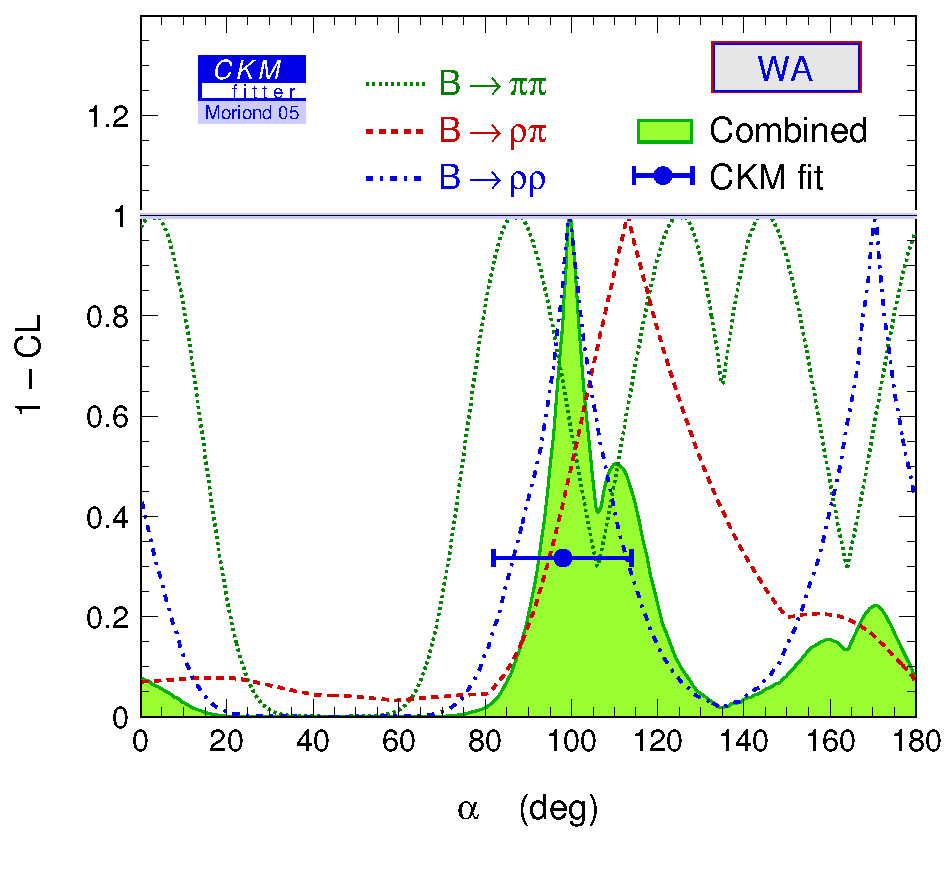
\includegraphics[width=\largefigwidth]{ckmfitter-alpha-combined}
%   \caption[CKM Fitter constraints on \alphaCKM.]%
%   {CKM Fitter constraints on \alphaCKM from combined \BToPiPi,
%     \BToRhoPi and \BToRhoRho decay analyses.}
%   \label{fig:CKMFitter}
% \end{figure}

\section{The \LHCb experiment}
\label{sec:LHCbInDetail}

Since both \bhadron{s} are preferentially produced in the same direction
and are forward-boosted along the beam-pipe, the detector is not required
to have full $4\pi$ solid-angle coverage. \LHCb takes advantage of this
by using a wedge-shaped single-arm detector with angular acceptance
\unit{10-300}{\mrad} in the horizontal (bending) plane~\cite{Amato:1998xt}.

\vspace{1cm}

\begin{center}
{\hspace{1mm}\Large\vdots\hspace{1cm}}
\end{center}

\vspace{1cm}

The detector is illustrated in \FigureRef{fig:LHCbCrossSection}, showing
the overall scale of the experiment and the surrounding cavern structure.

\begin{sidewaysfigure}
  \begin{center}
  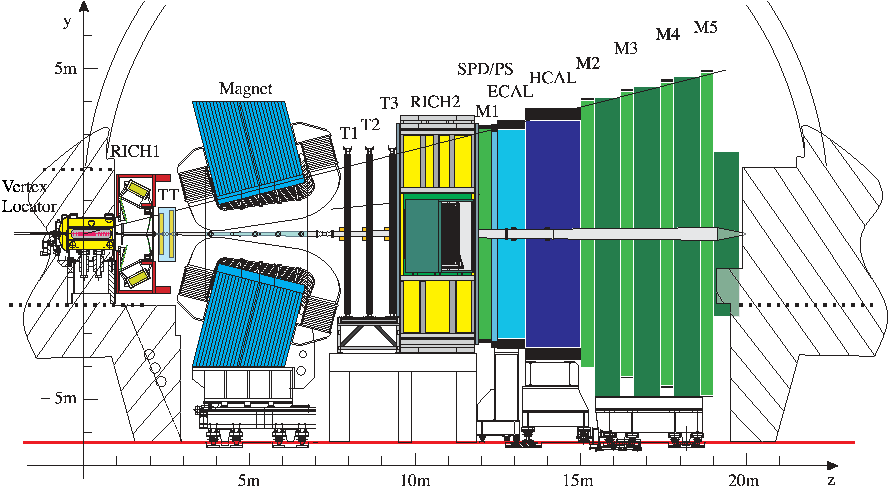
\includegraphics[width=0.8\textheight]{lhcb-detector-cross-section}
  \caption[Cross-section view of \LHCb, cut in the non-bending $y$--$z$ plane]%
    {Cross-section view of \LHCb, cut in the non-bending $y$--$z$ plane.}
  \label{fig:LHCbCrossSection}
  \end{center}
\end{sidewaysfigure}

The single-sided detector design was chosen in preference to a two-armed
design since the detector dimensions are restricted by the layout of the
IP8 (ex-Delphi) cavern in which \LHCb is located. Using all the available
space for a single-arm spectrometer more than compensates in performance
for the \about{50\percent} drop in luminosity.

\section{The \Cerenkov mechanism}
A Huygens construction in terms of spherical shells of probability for photon
emission as the particle progresses along its track shows an effective
``shock-front'' of \Cerenkov emission. This corresponds to an emission cone of
opening angle \thetaCerenkov around the momentum vector for each point on the
track,
%
\begin{subequations}
  \label{eq:cosThetaCk}
  \begin{equation}
    \cos\,\thetaCerenkov  &= \frac{1}{n \beta} +
                             \frac{\hbar k}{2p}%
                             \parenths{ 1 - \frac{1}{n^2} } \\
                          &\,\sim \frac{1}{n \beta}%
    \label{eq:cosThetaCkApprox}
  \end{equation}
\end{subequations}
%
where $\beta \equiv v/c$, the relativistic velocity fraction.

\section{Trigger system}
\label{sec:triggers}
An overview of the \LHCb trigger characteristics broken down by level
is shown in \Table~\ref{tab:TriggerDetails}.

\begin{table}[bp]
  \begin{tabular}{lllll}
                & L0              & L1              & HLT             \\
    \midrule\\
    Input rate  & \unit{40}{\MHz} & \unit{1}{\MHz}  & \unit{40}{\kHz} \\
    Output rate & \unit{1}{\MHz}  & \unit{40}{\kHz} & \unit{2}{\kHz}  \\
    Location    & On detector     & Counting room   & Counting room   \\
  \end{tabular}
  \caption{Characteristics of the trigger levels and offline analysis.}
  \label{tab:TriggerDetails}
\end{table}

  \chapter{Continued captions}
\label{chap:ContCaptions}

Here are some funky floats using ``continued captions'', i.e. for a semantically
collected group of float contents which are too numerous to fit into a single
float, such as the pretty circles in the following figure:

\newcommand{\circleimg}[1]{%
\begin{tikzpicture}
  \draw[color=black,fill=#1,thick] (1,0) circle (1.5cm);
\end{tikzpicture}%
}

\begin{figure}[hb]
  \subfloat[][Example 1a]{\label{fig:cc1a}\circleimg{red!80}}\quad
  \subfloat[][Example 1b]{\label{fig:cc1b}\circleimg{green!70!yellow}}\quad
  \subfloat[][Example 1c]{\label{fig:cc1c}\circleimg{blue!80}}\quad
  \subfloat[][Example 1d]{\label{fig:cc1d}\circleimg{orange!80!yellow}}
  \caption{Demonstration of \texttt{subfig} continued captions.}
  \label{fig:cc1}
\end{figure}

\begin{figure}[p]
  \ContinuedFloat
  \subfloat[][Example 1e]{\label{fig:cc1e}\circleimg{violet}}\quad
  \subfloat[][Example 1f]{\label{fig:cc1f}\circleimg{cyan}}\quad
  \subfloat[][Example 1g]{\label{fig:cc1g}\circleimg{magenta}}\quad
  \subfloat[][Example 1h]{\label{fig:cc1h}\circleimg{yellow}}
  \caption[]{Demonstration of \texttt{subfig} continued captions (continued).}
\end{figure}

\noindent
This mechanism means that the same float label is used for both pages of
floats. Note that we can refer to \FigureRef{fig:cc1} in general, or to
\FigureRef{fig:cc1g} on \PageRef{fig:cc1g} in particular!

\noindent
Just for the hell of it, let's also refer to \SectionRef{sec:neutralmixing}.

  %% To ignore a specific chapter while working on another, making the build faster, comment it out:
  %\input{chap4}
\end{mainmatter}

%% Produce the appendices
\begin{appendices}
  %% The "\appendix" call has already been made in the declaration
%% of the "appendices" environment (see thesis.tex).
\chapter{Appendices}
\label{app:appendices}

\section{Characterisation of the signal and control regions}
\label{app:charac}

Extra data-\MC comparisons of the key analysis variables in each of
the signal and control regions of the analysis are included in this
section

% \clearpage
% \subsection{Yields and distributions for the muon + jets control sample}

\begin{figure}
    \begin{center}
        \subfloat {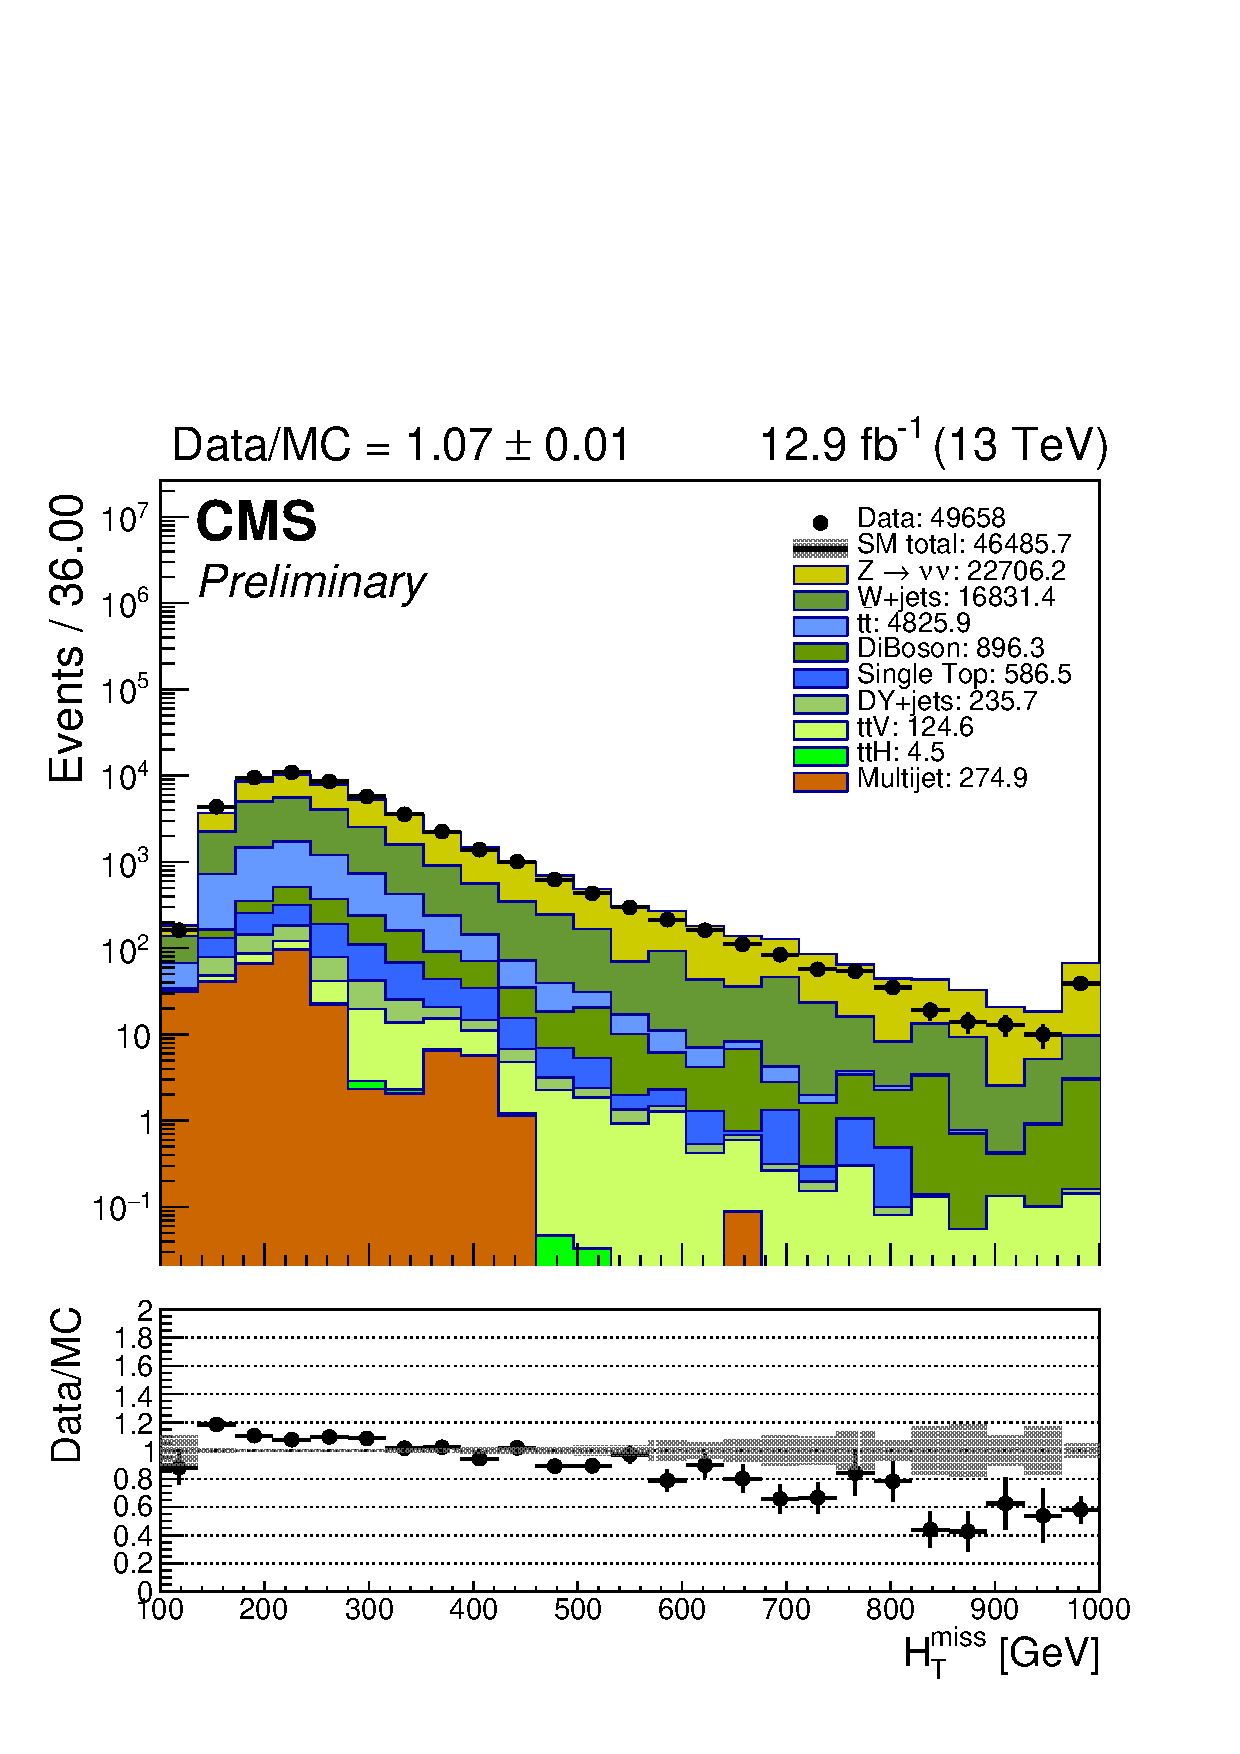
\includegraphics[width=0.5\textwidth]{figs/analysis/distributions/Signal/mht40_pt_sym.pdf}} ~~
        \subfloat {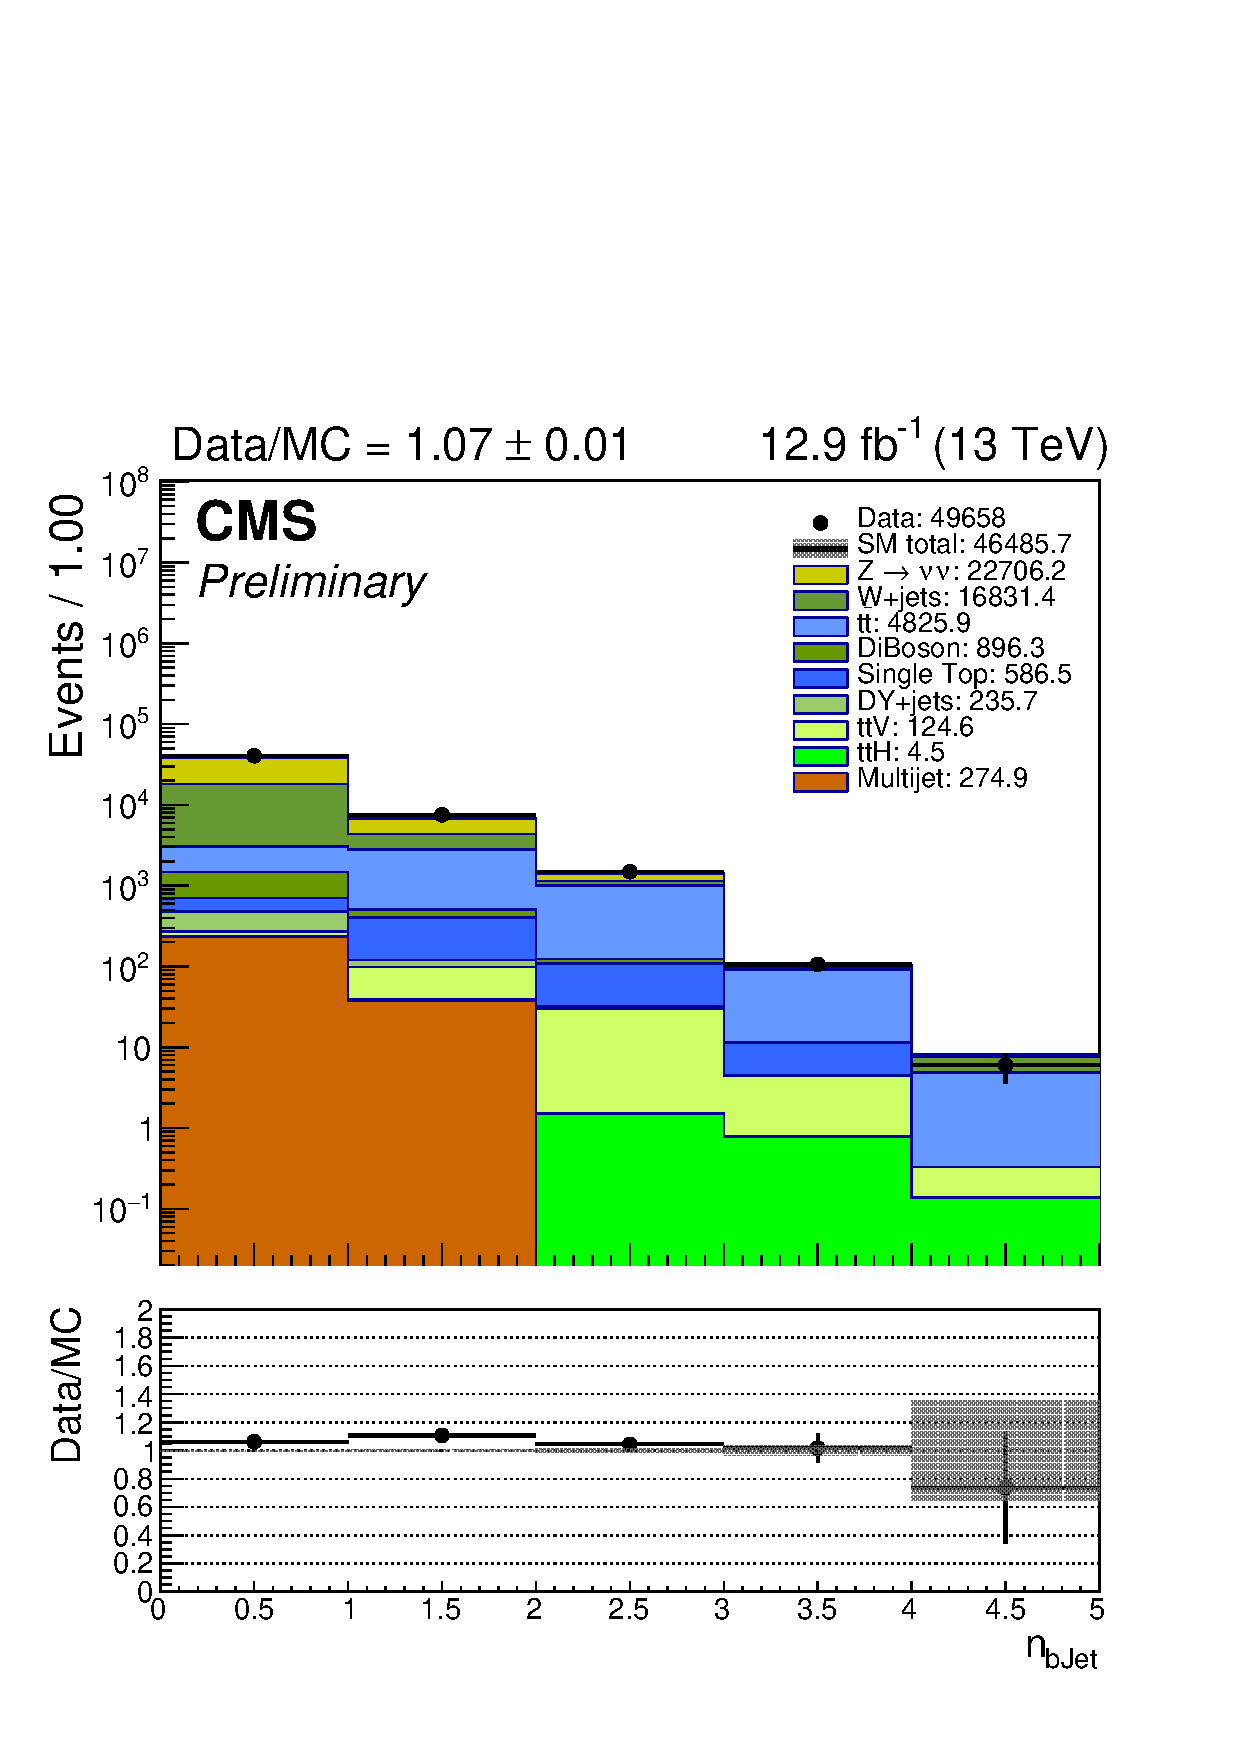
\includegraphics[width=0.5\textwidth]{figs/analysis/distributions/Signal/nBJet40_sym.pdf}} \\
        \caption{Key analysis variables for hadronic signal region (symmetric \njet bins)}
        \label{fig:distribution_signal_sym}
    \end{center}
\end{figure}

\clearpage
\begin{figure}
    \begin{center}
        \subfloat {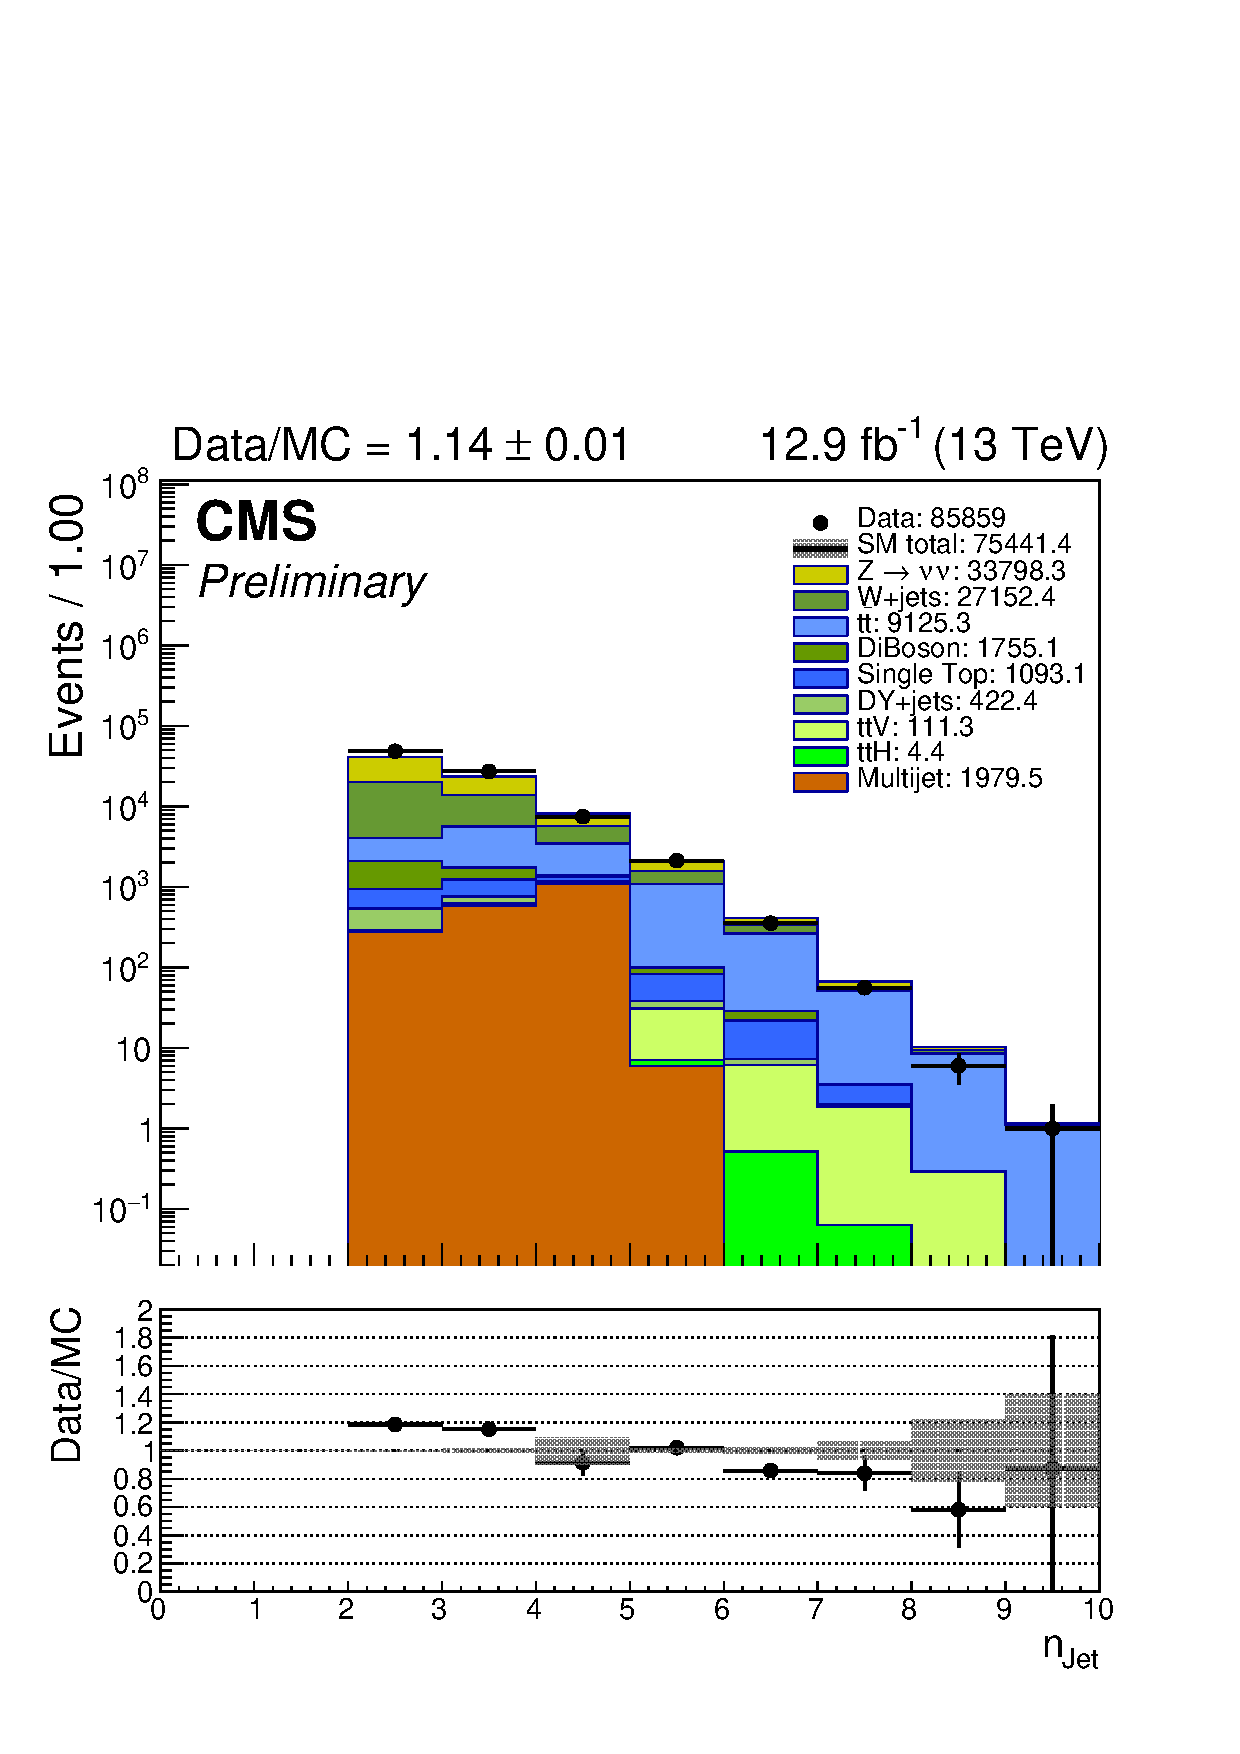
\includegraphics[width=0.5\textwidth]{figs/analysis/distributions/Signal/nJet40_asym.pdf}} ~~
        \subfloat {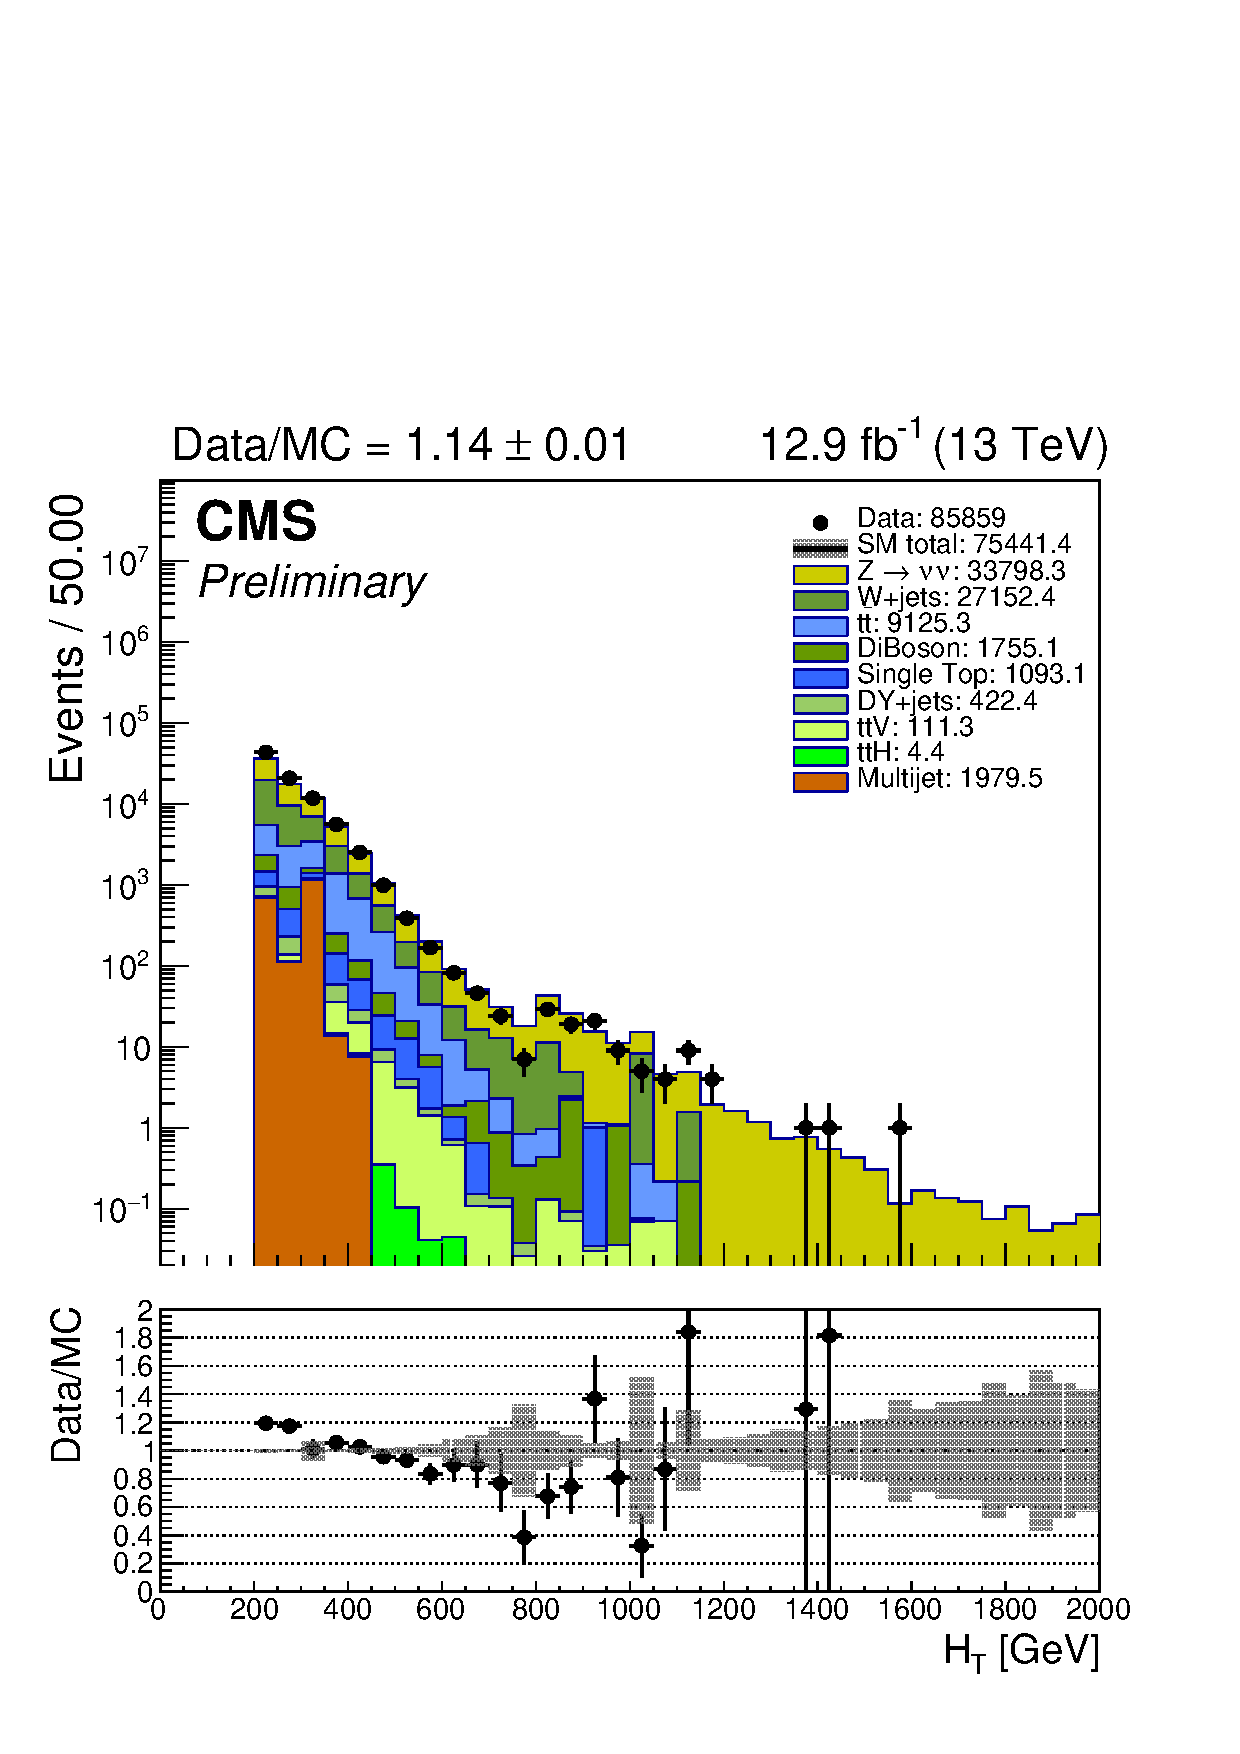
\includegraphics[width=0.5\textwidth]{figs/analysis/distributions/Signal/ht40_asym.pdf}} \\
        \subfloat {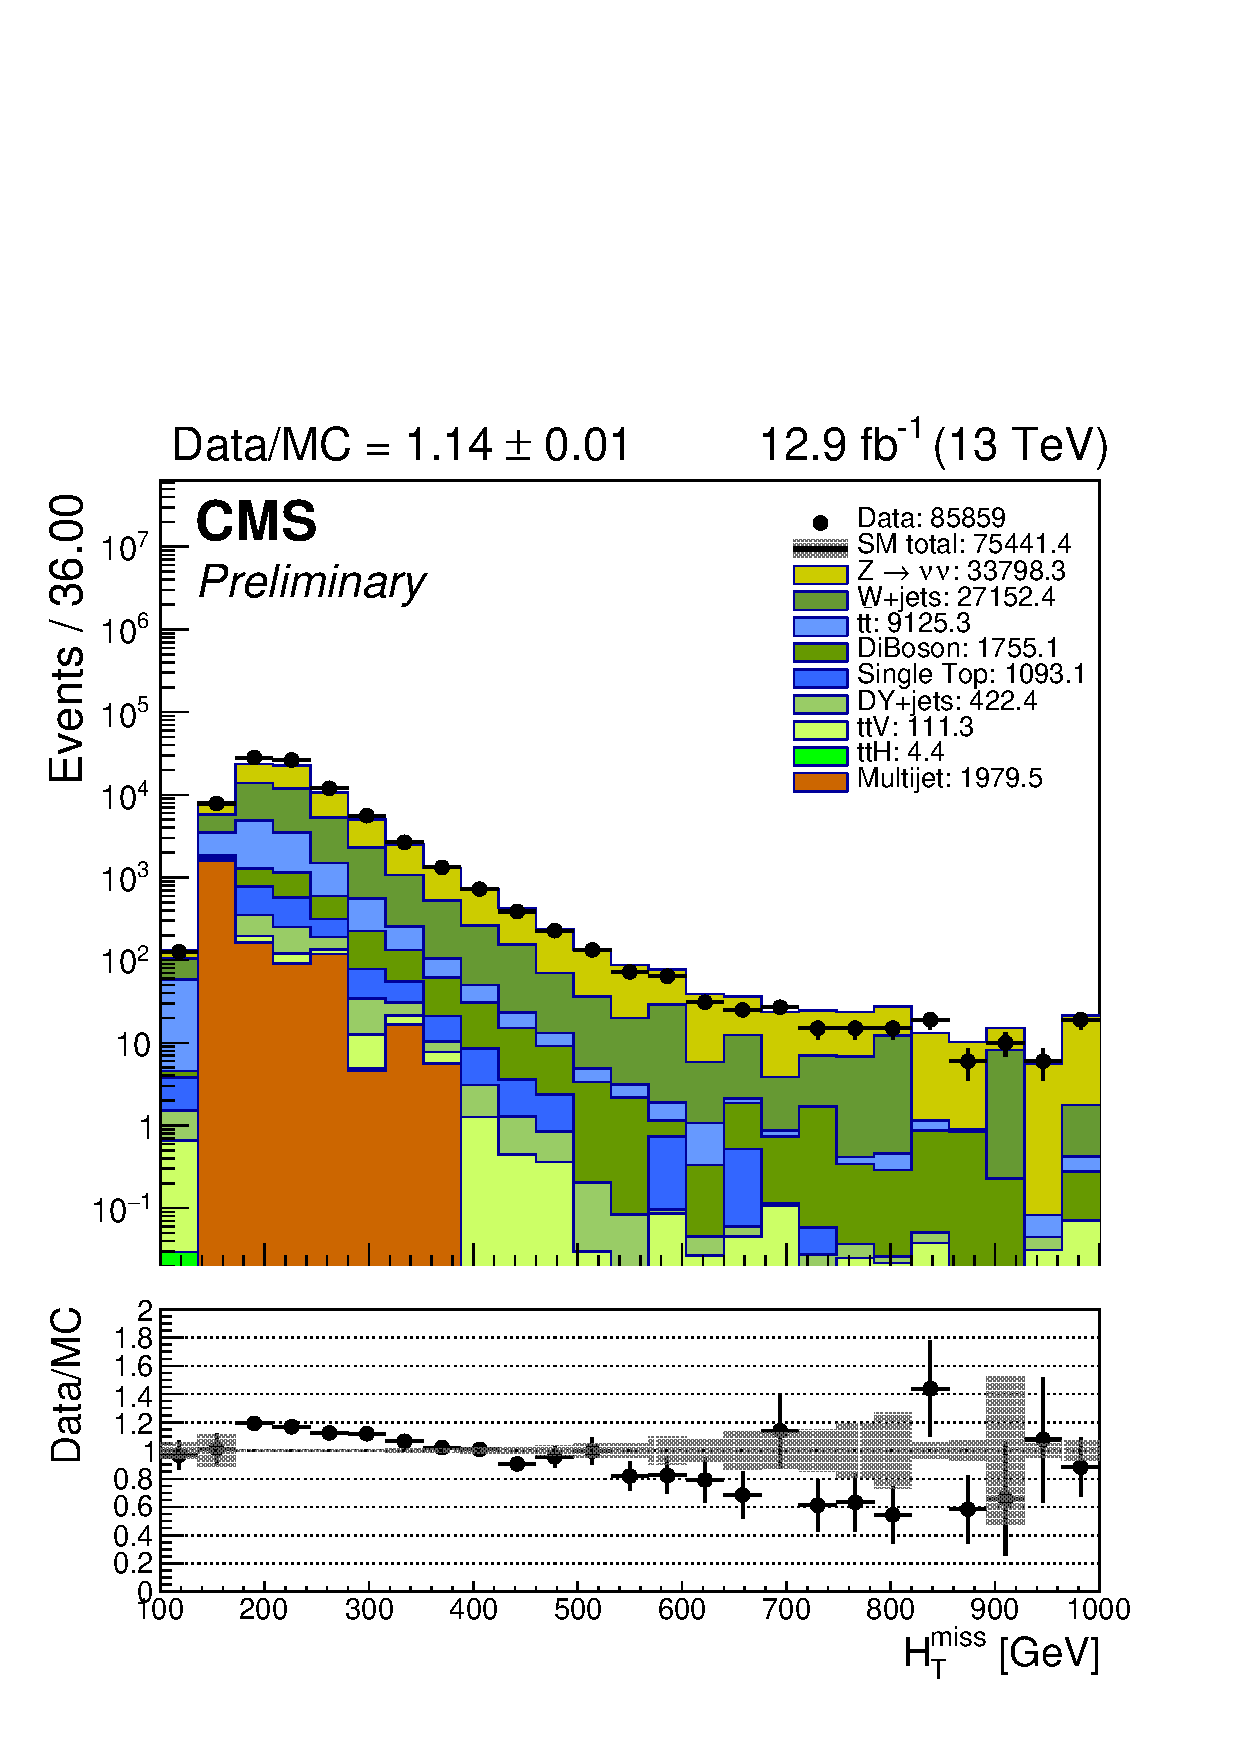
\includegraphics[width=0.5\textwidth]{figs/analysis/distributions/Signal/mht40_pt_asym.pdf}} ~~
        \subfloat {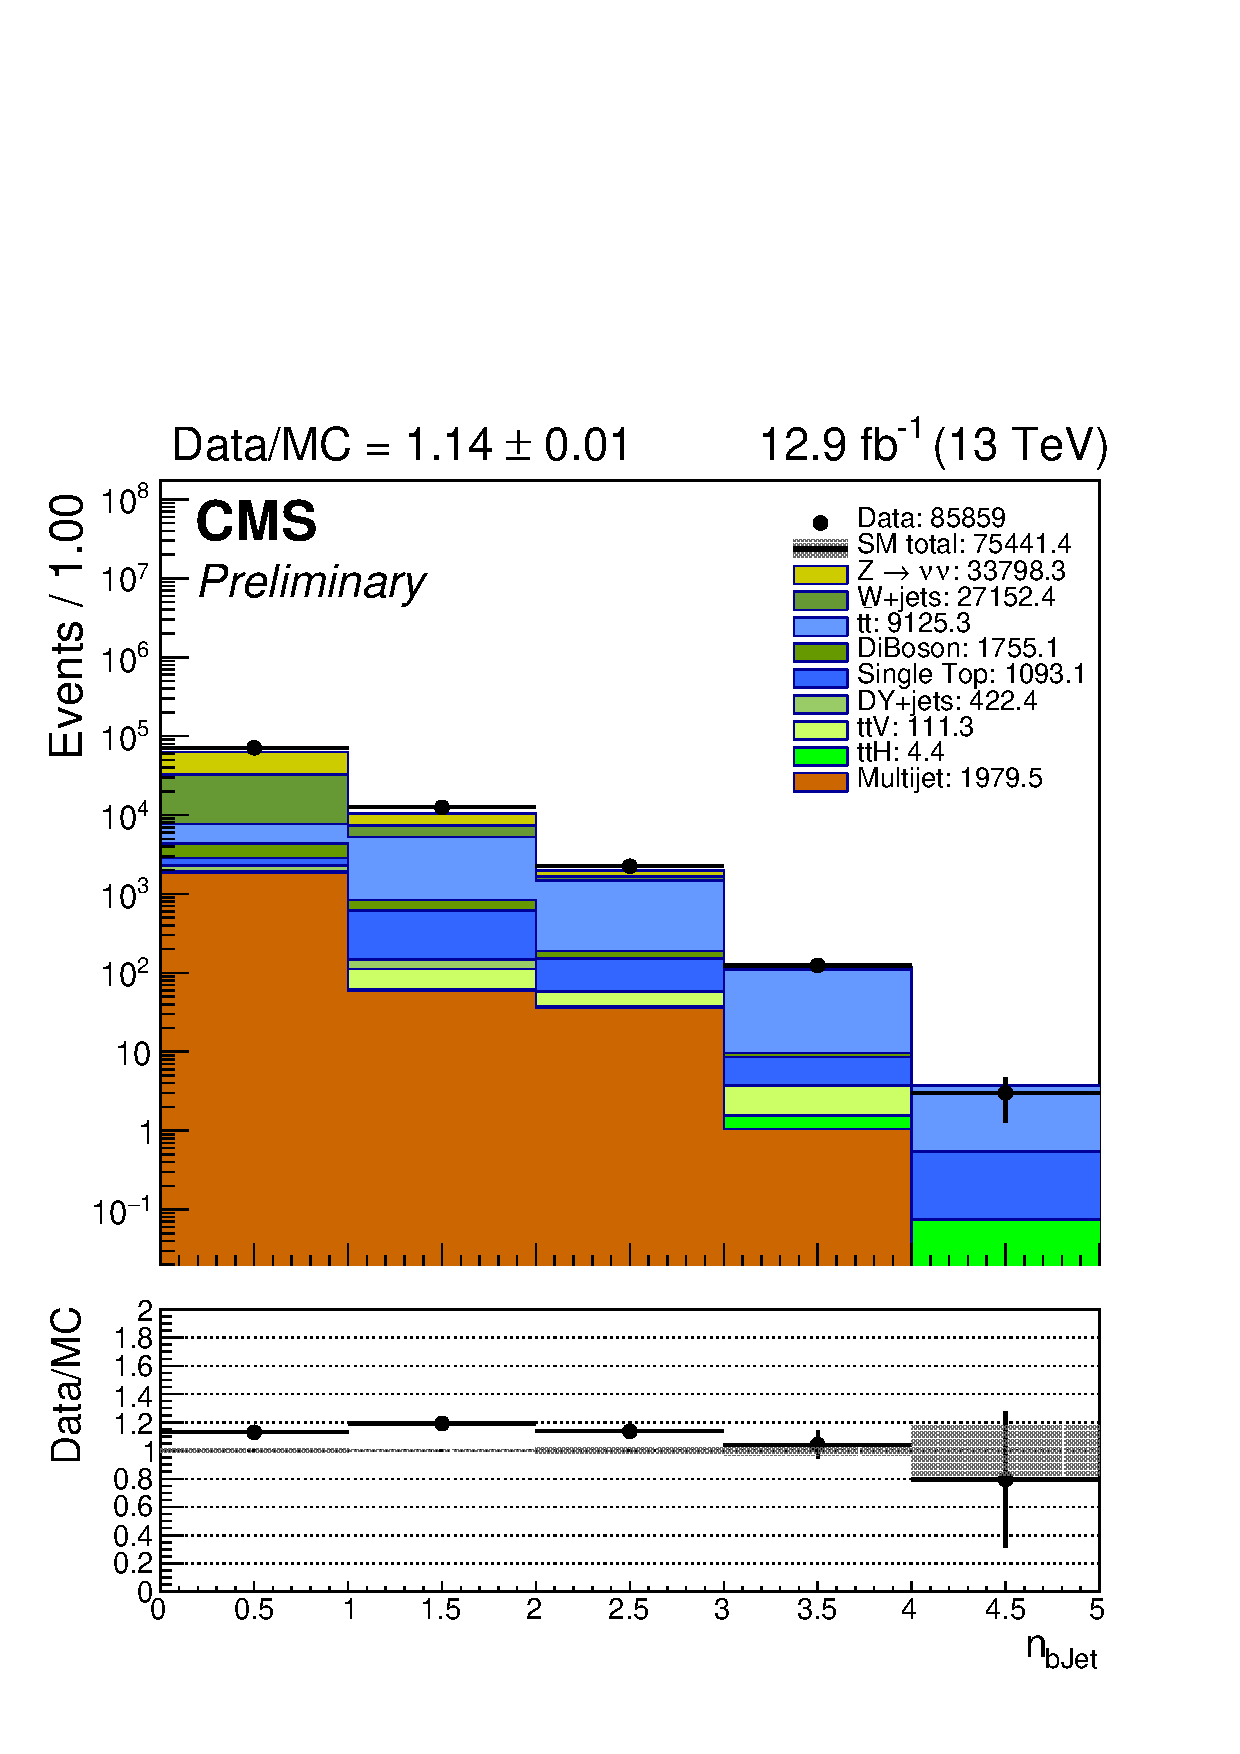
\includegraphics[width=0.5\textwidth]{figs/analysis/distributions/Signal/nBJet40_asym.pdf}} \\
        \caption{Key analysis variables for hadronic signal region (asymmetric \njet bins)}
        \label{fig:distribution_signal_asym}
    \end{center}
\end{figure}

\clearpage
\begin{figure}
    \begin{center}
        \subfloat {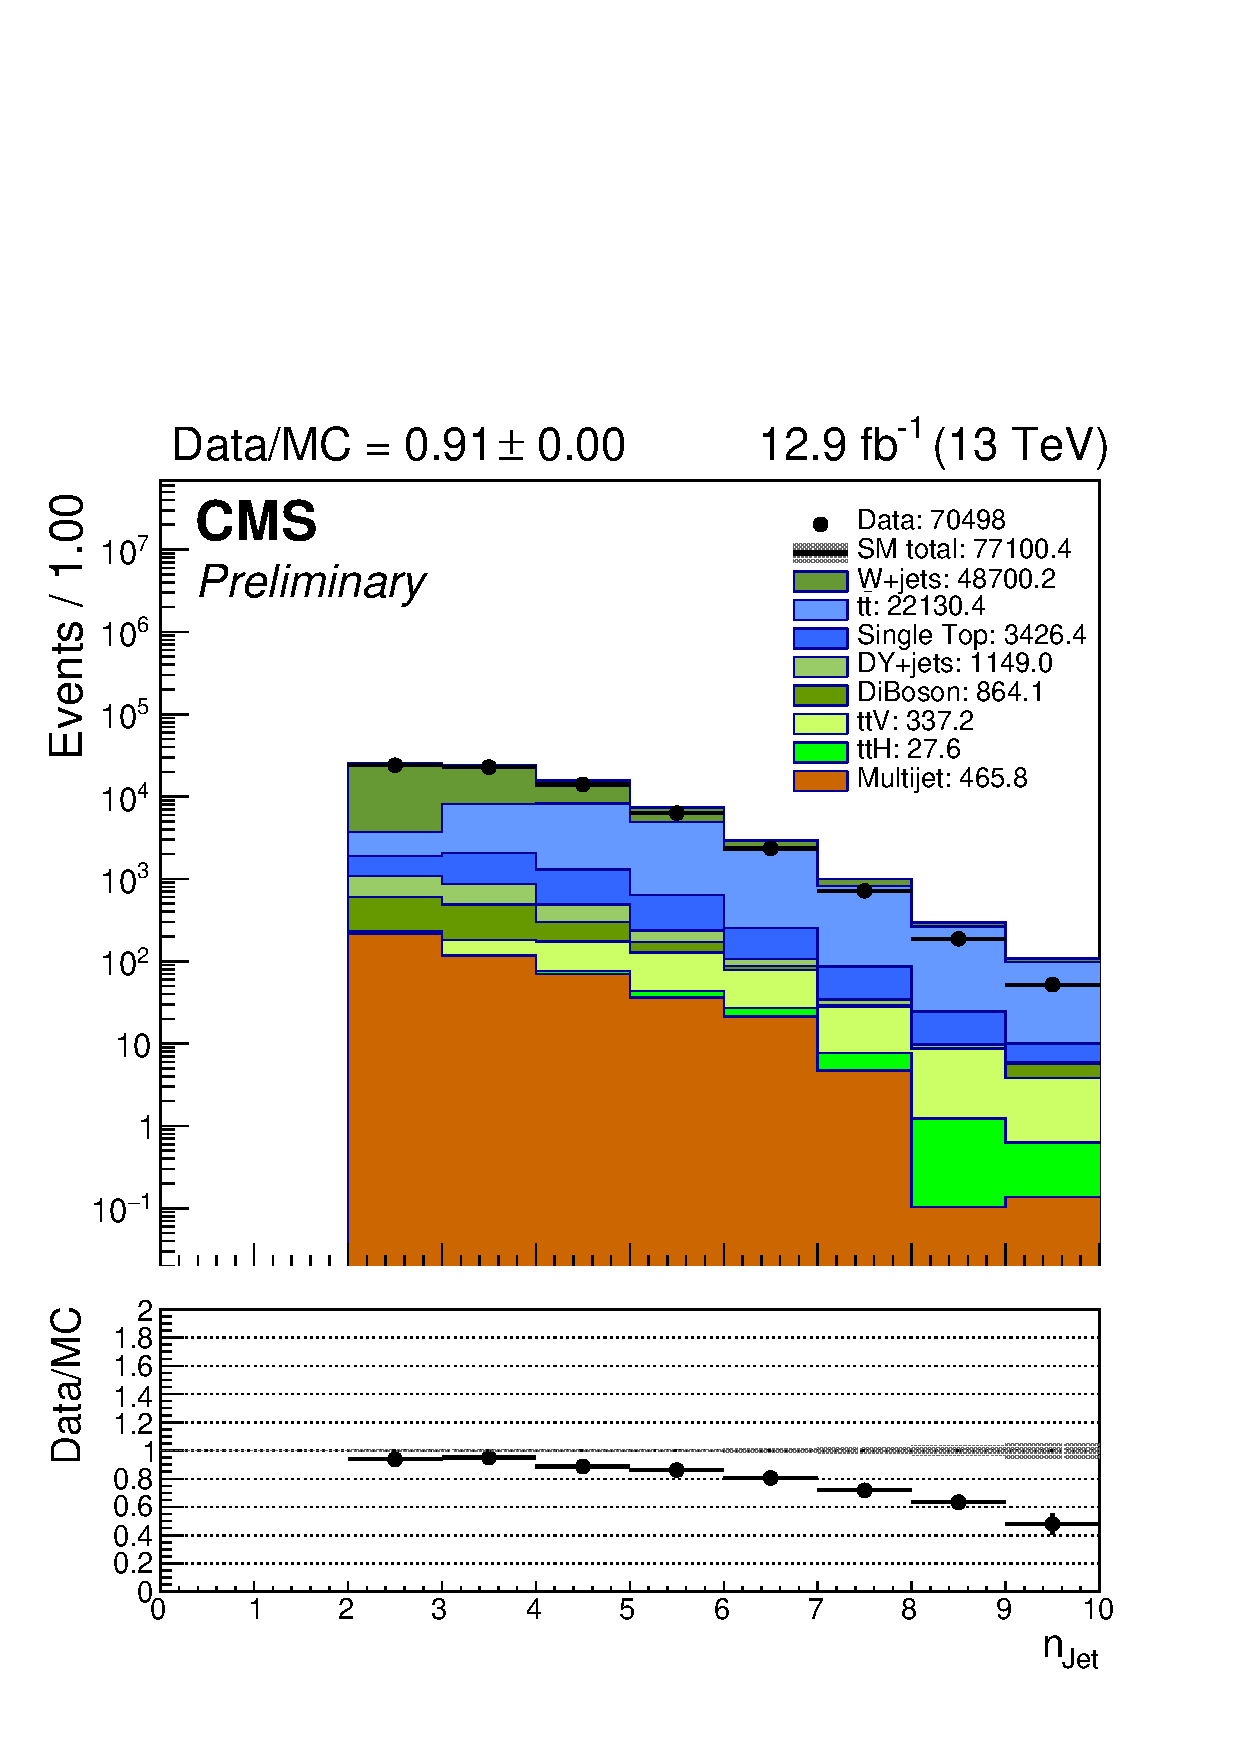
\includegraphics[width=0.5\textwidth]{figs/analysis/distributions/SingleMu/nJet40_sym.pdf}} ~~
        \subfloat {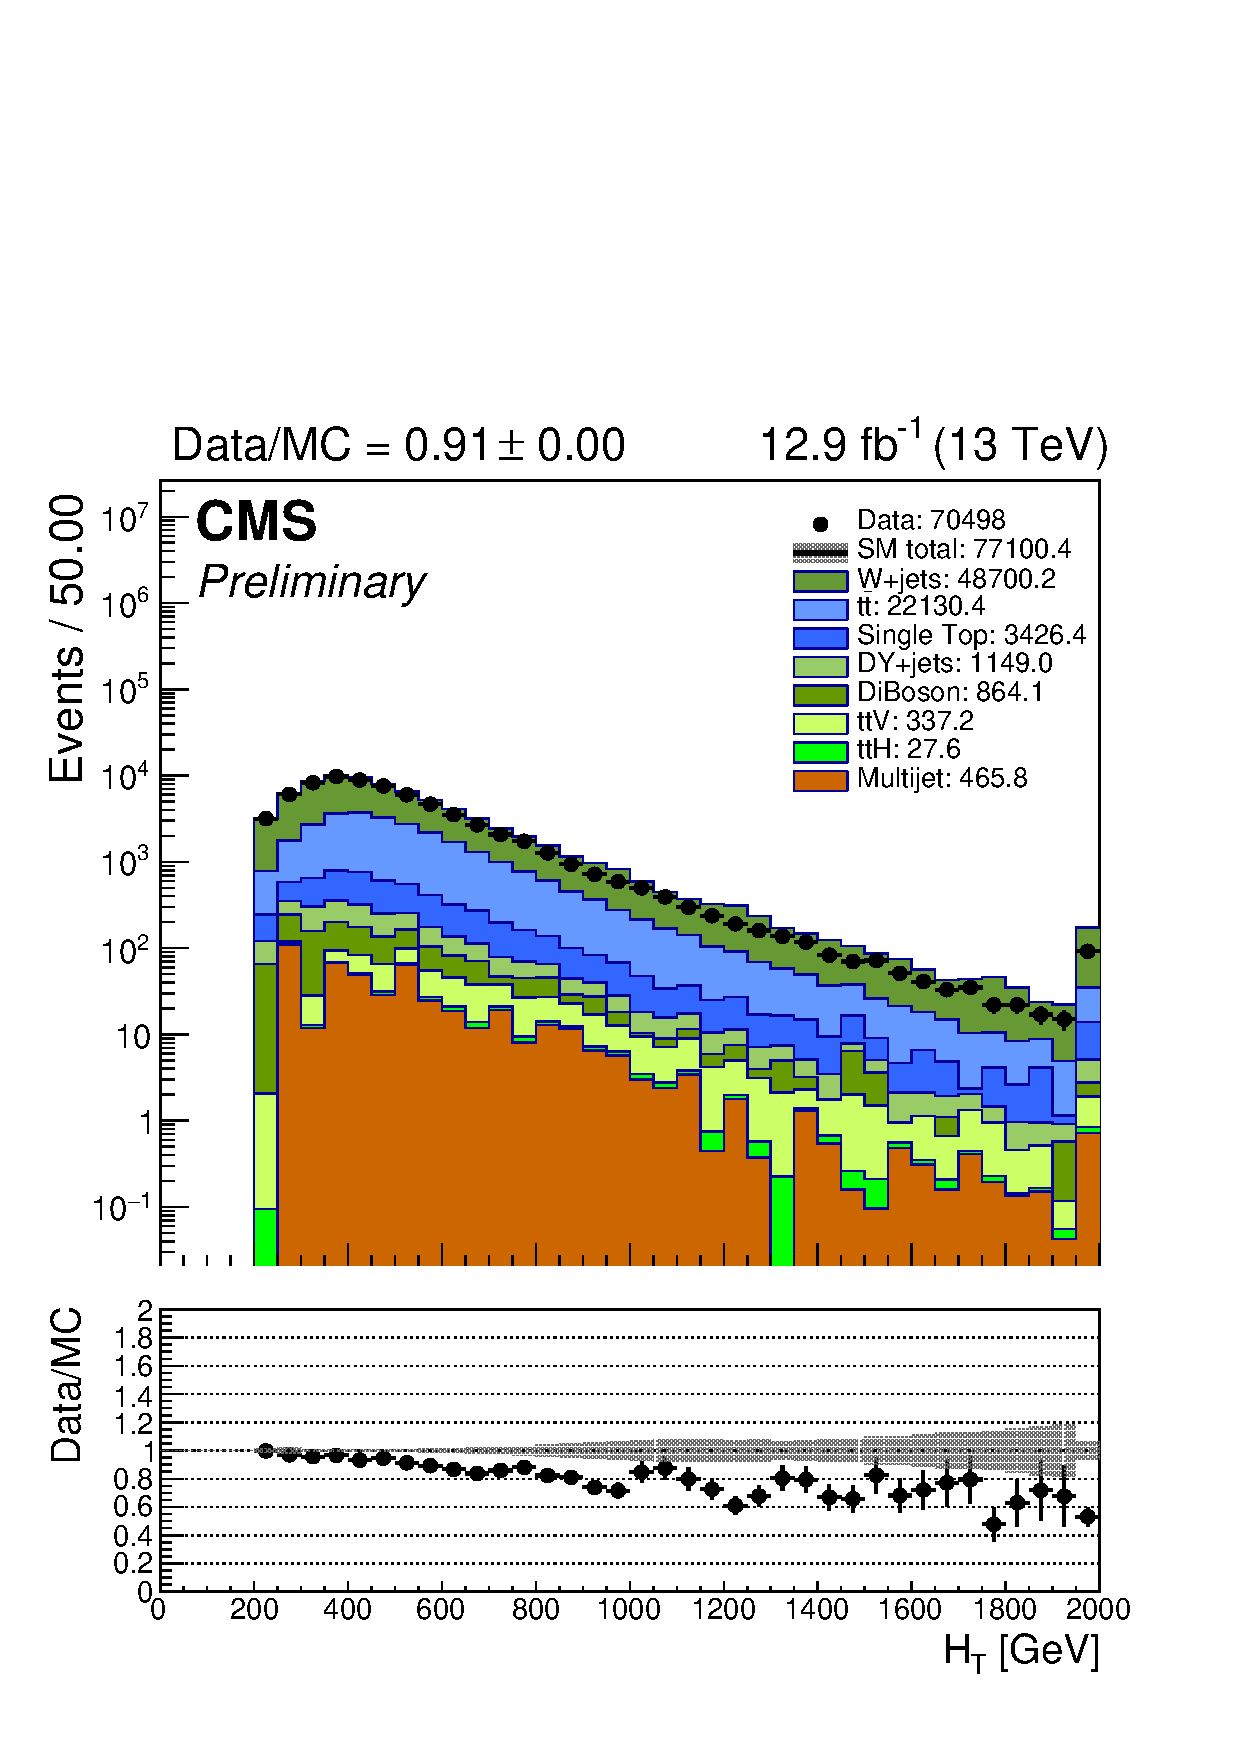
\includegraphics[width=0.5\textwidth]{figs/analysis/distributions/SingleMu/ht40_sym.pdf}} \\
        \subfloat {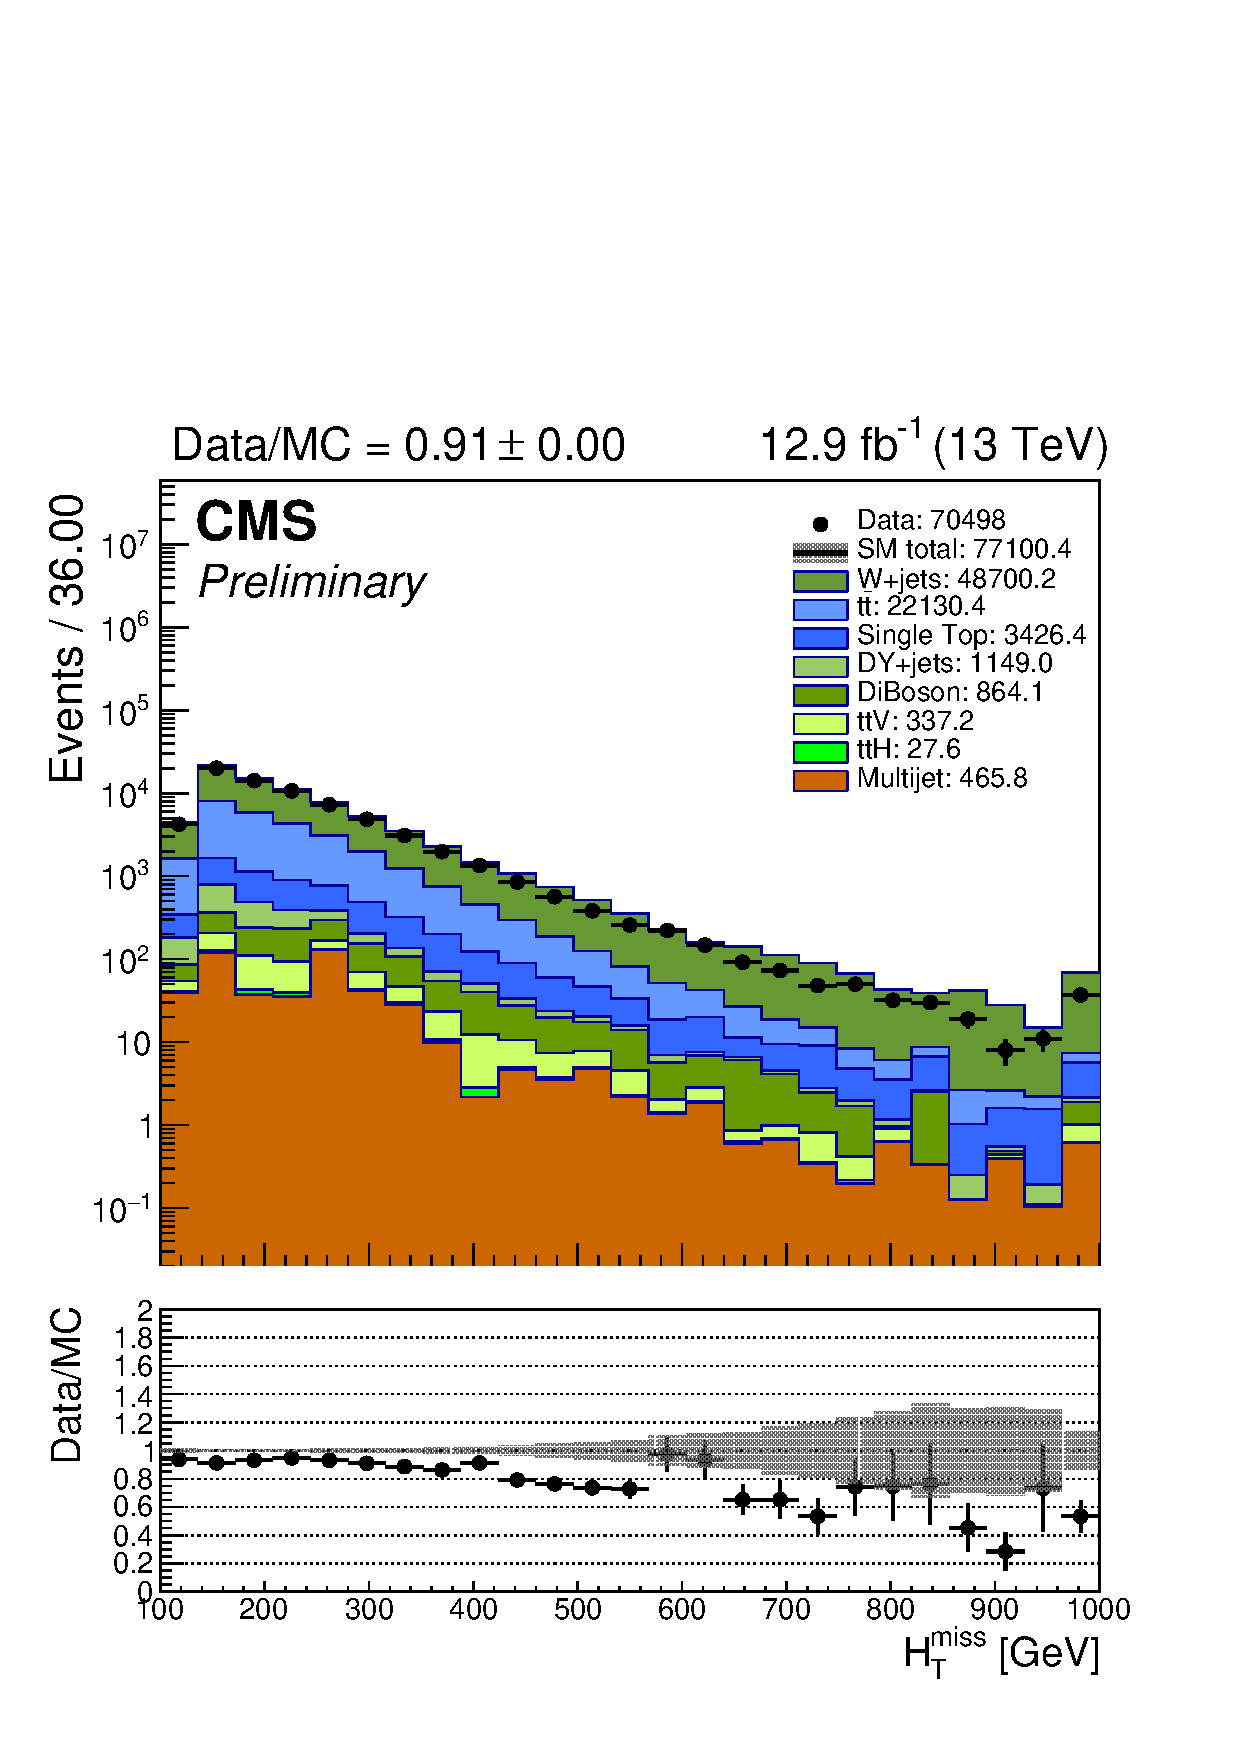
\includegraphics[width=0.5\textwidth]{figs/analysis/distributions/SingleMu/mht40_pt_sym.pdf}} ~~
        \subfloat {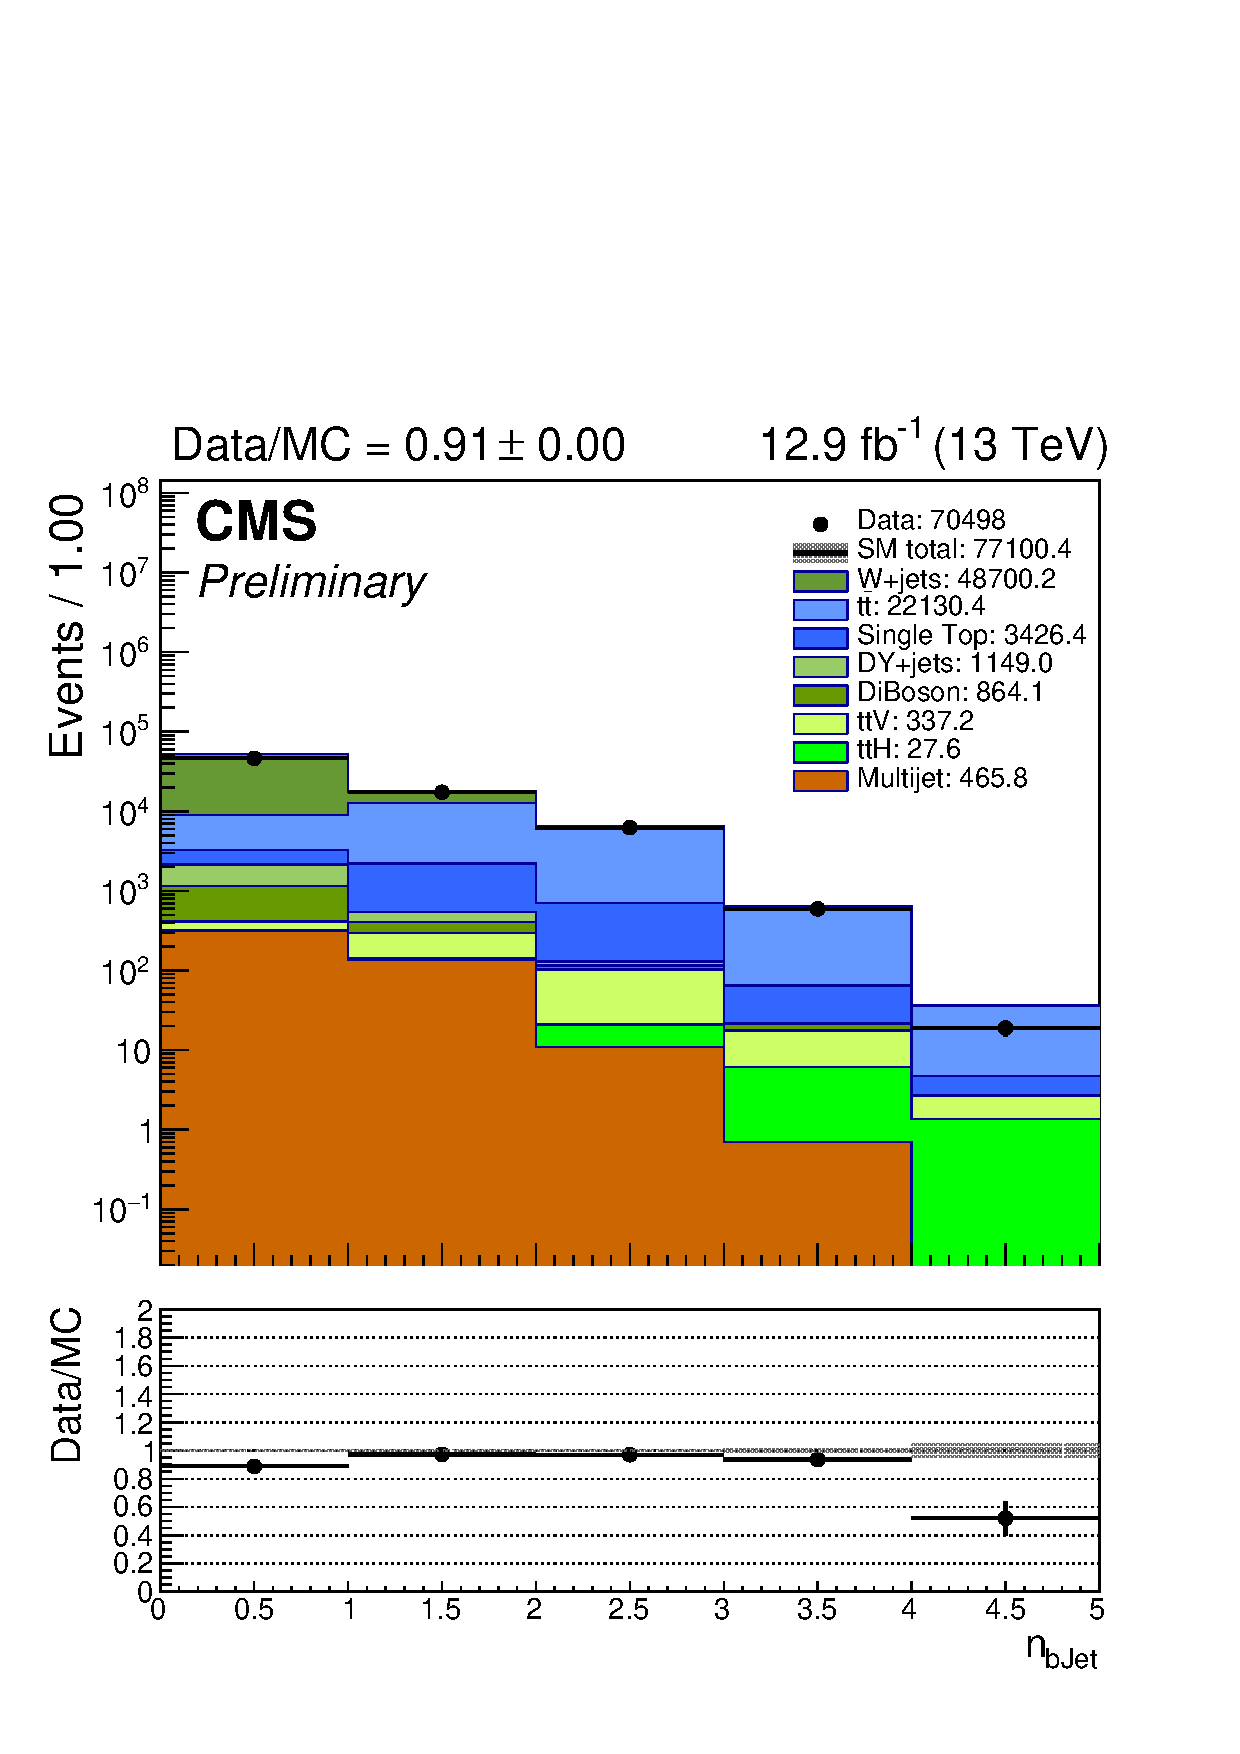
\includegraphics[width=0.5\textwidth]{figs/analysis/distributions/SingleMu/nBJet40_sym.pdf}} \\
        \caption{Key analysis variables for single muon control region (symmetric \njet bins)}
        \label{fig:distribution_singlemu_sym}
    \end{center}
\end{figure}

\clearpage
\begin{figure}
    \begin{center}
        \subfloat {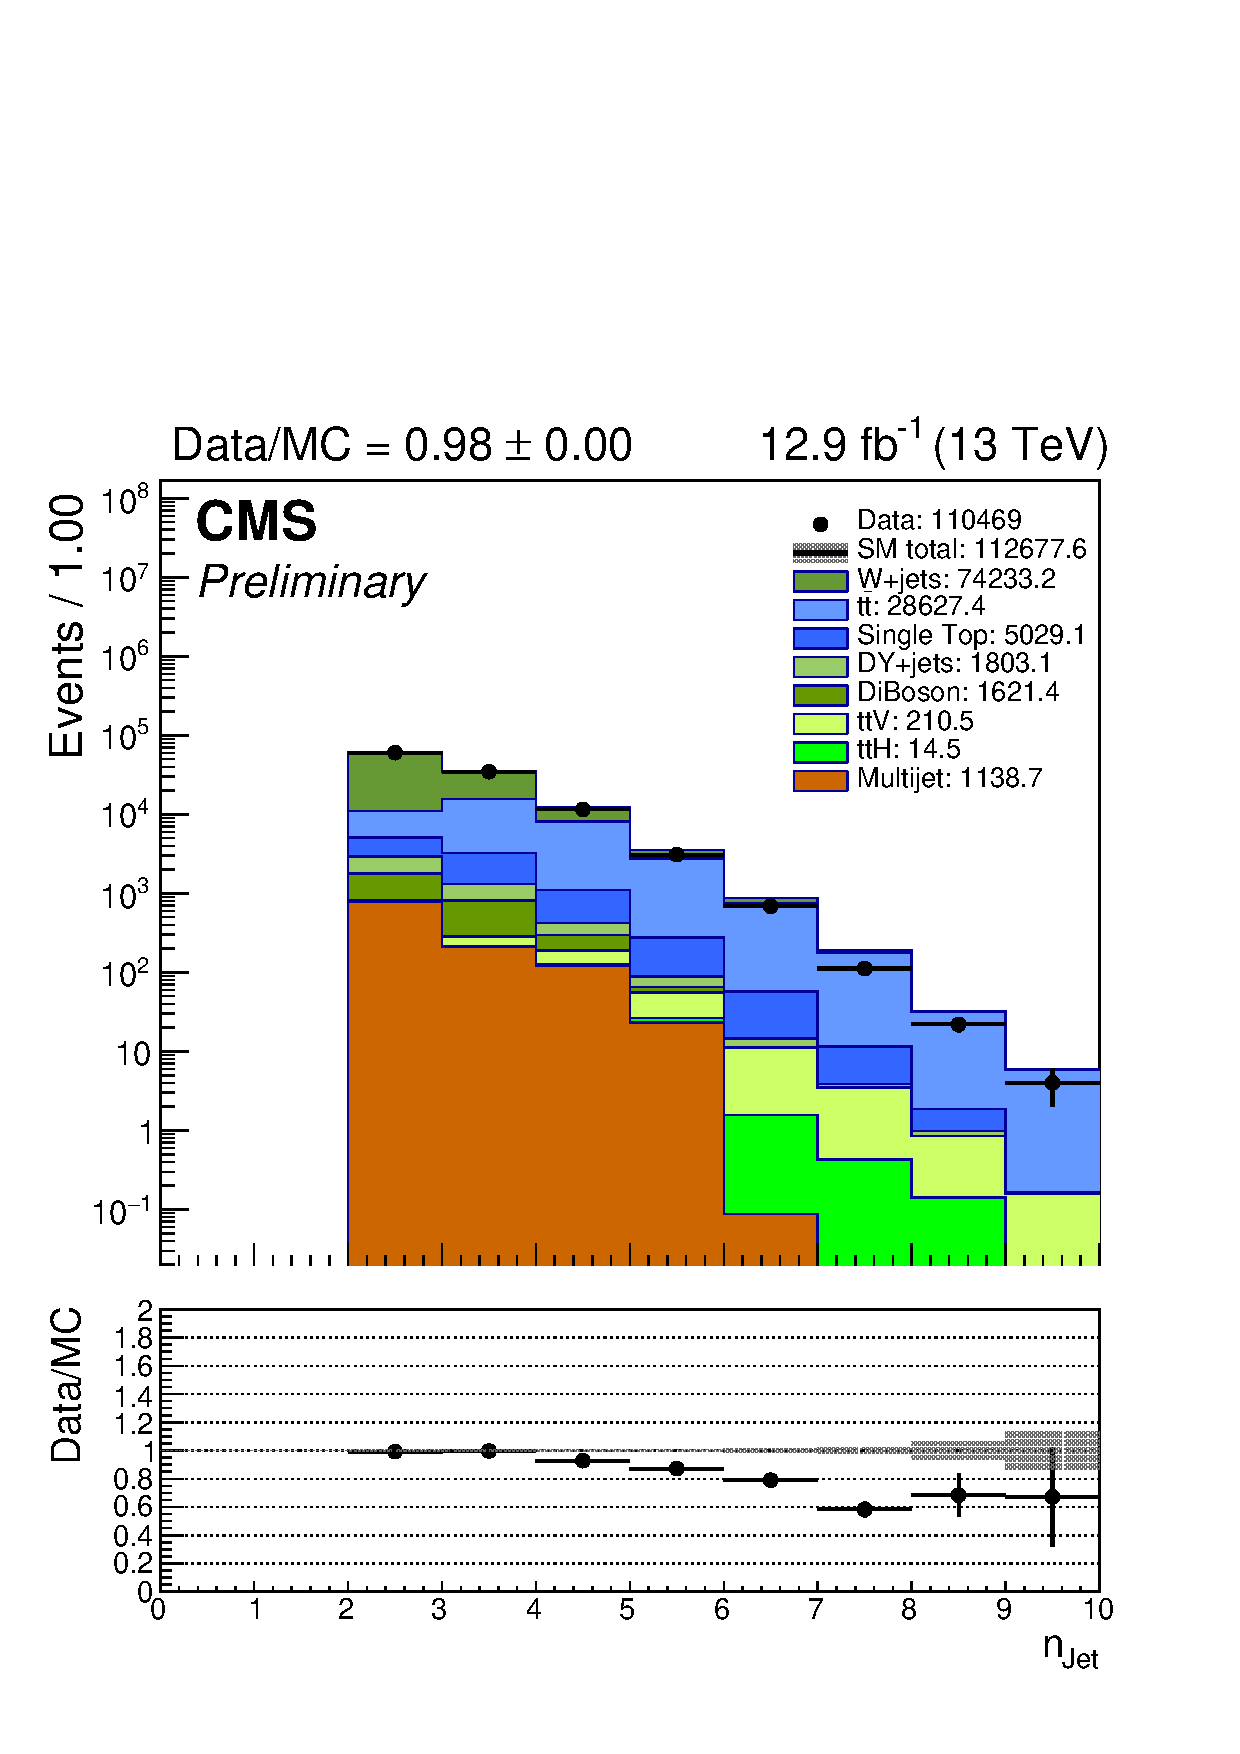
\includegraphics[width=0.5\textwidth]{figs/analysis/distributions/SingleMu/nJet40_asym.pdf}} ~~
        \subfloat {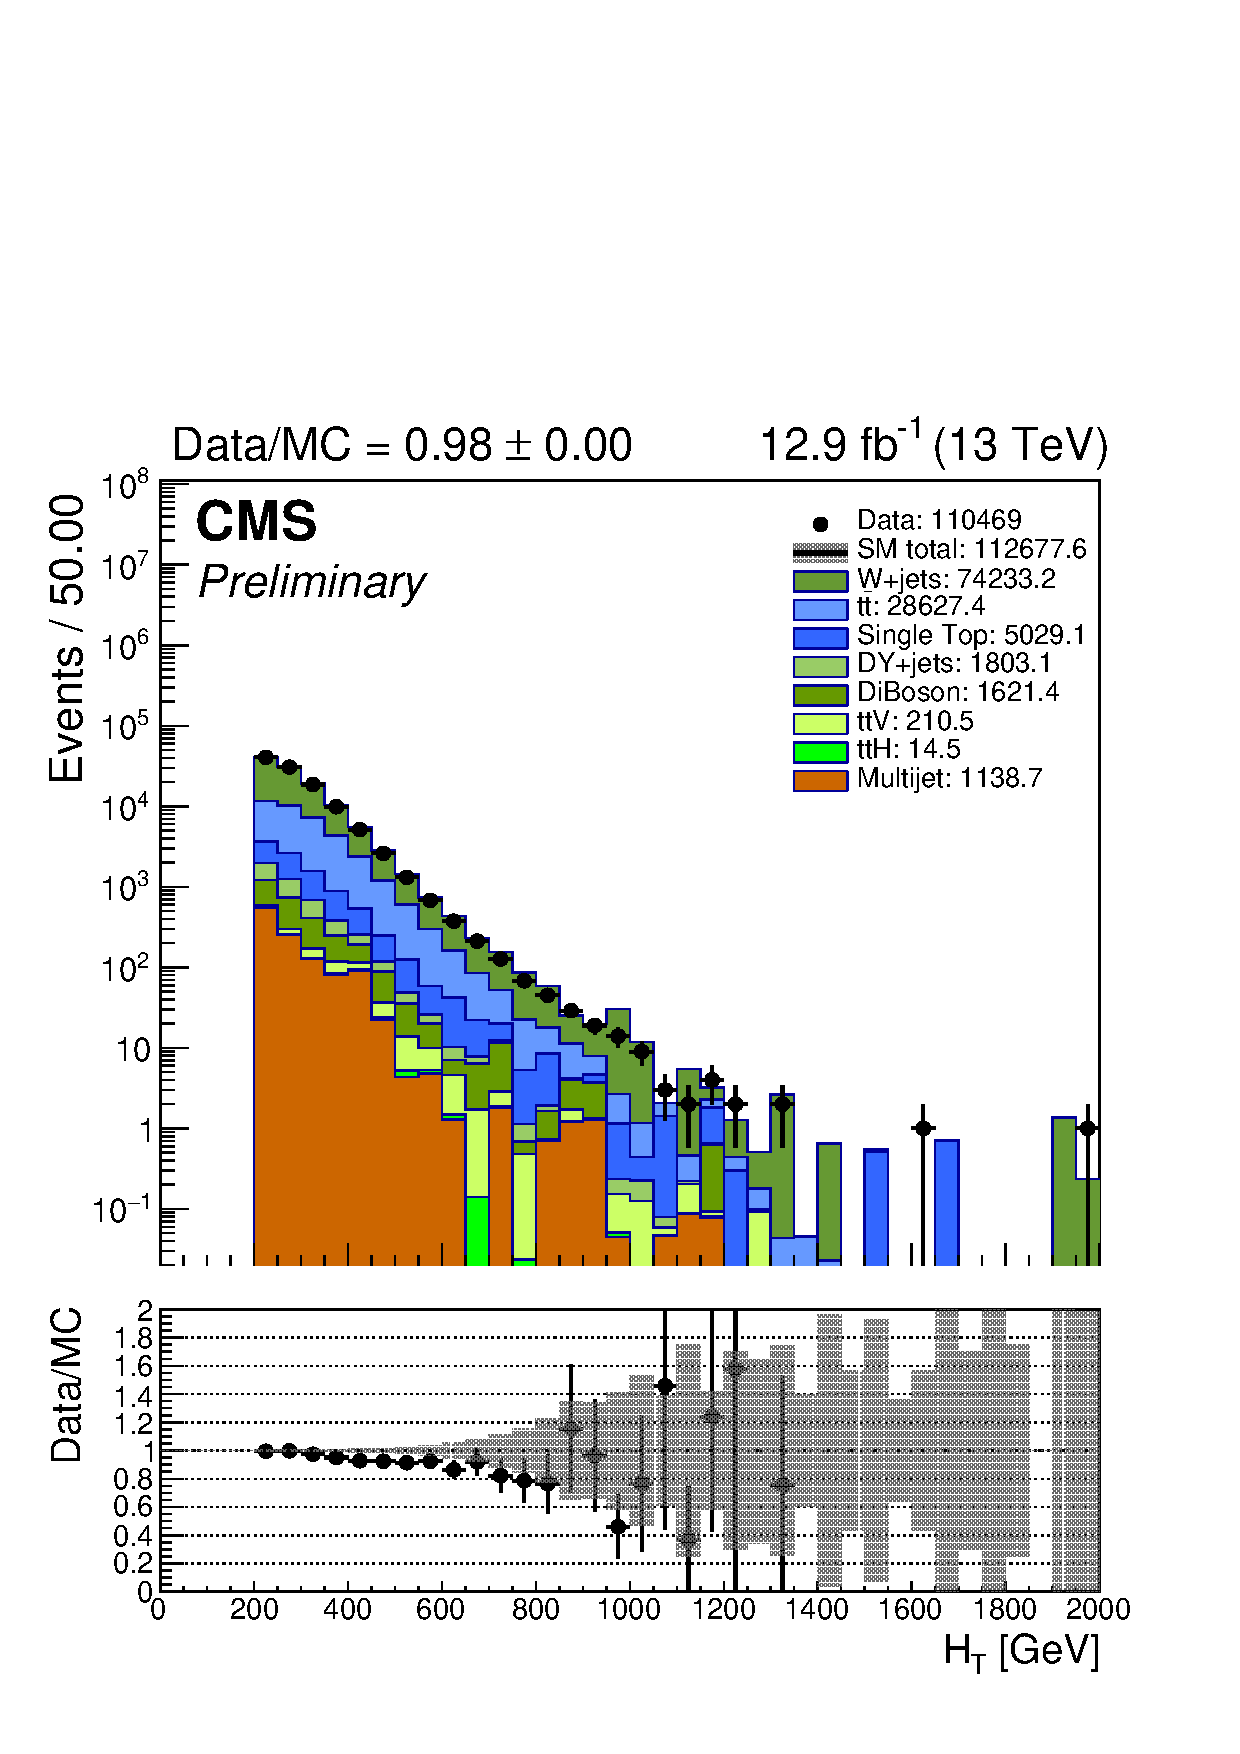
\includegraphics[width=0.5\textwidth]{figs/analysis/distributions/SingleMu/ht40_asym.pdf}} \\
        \subfloat {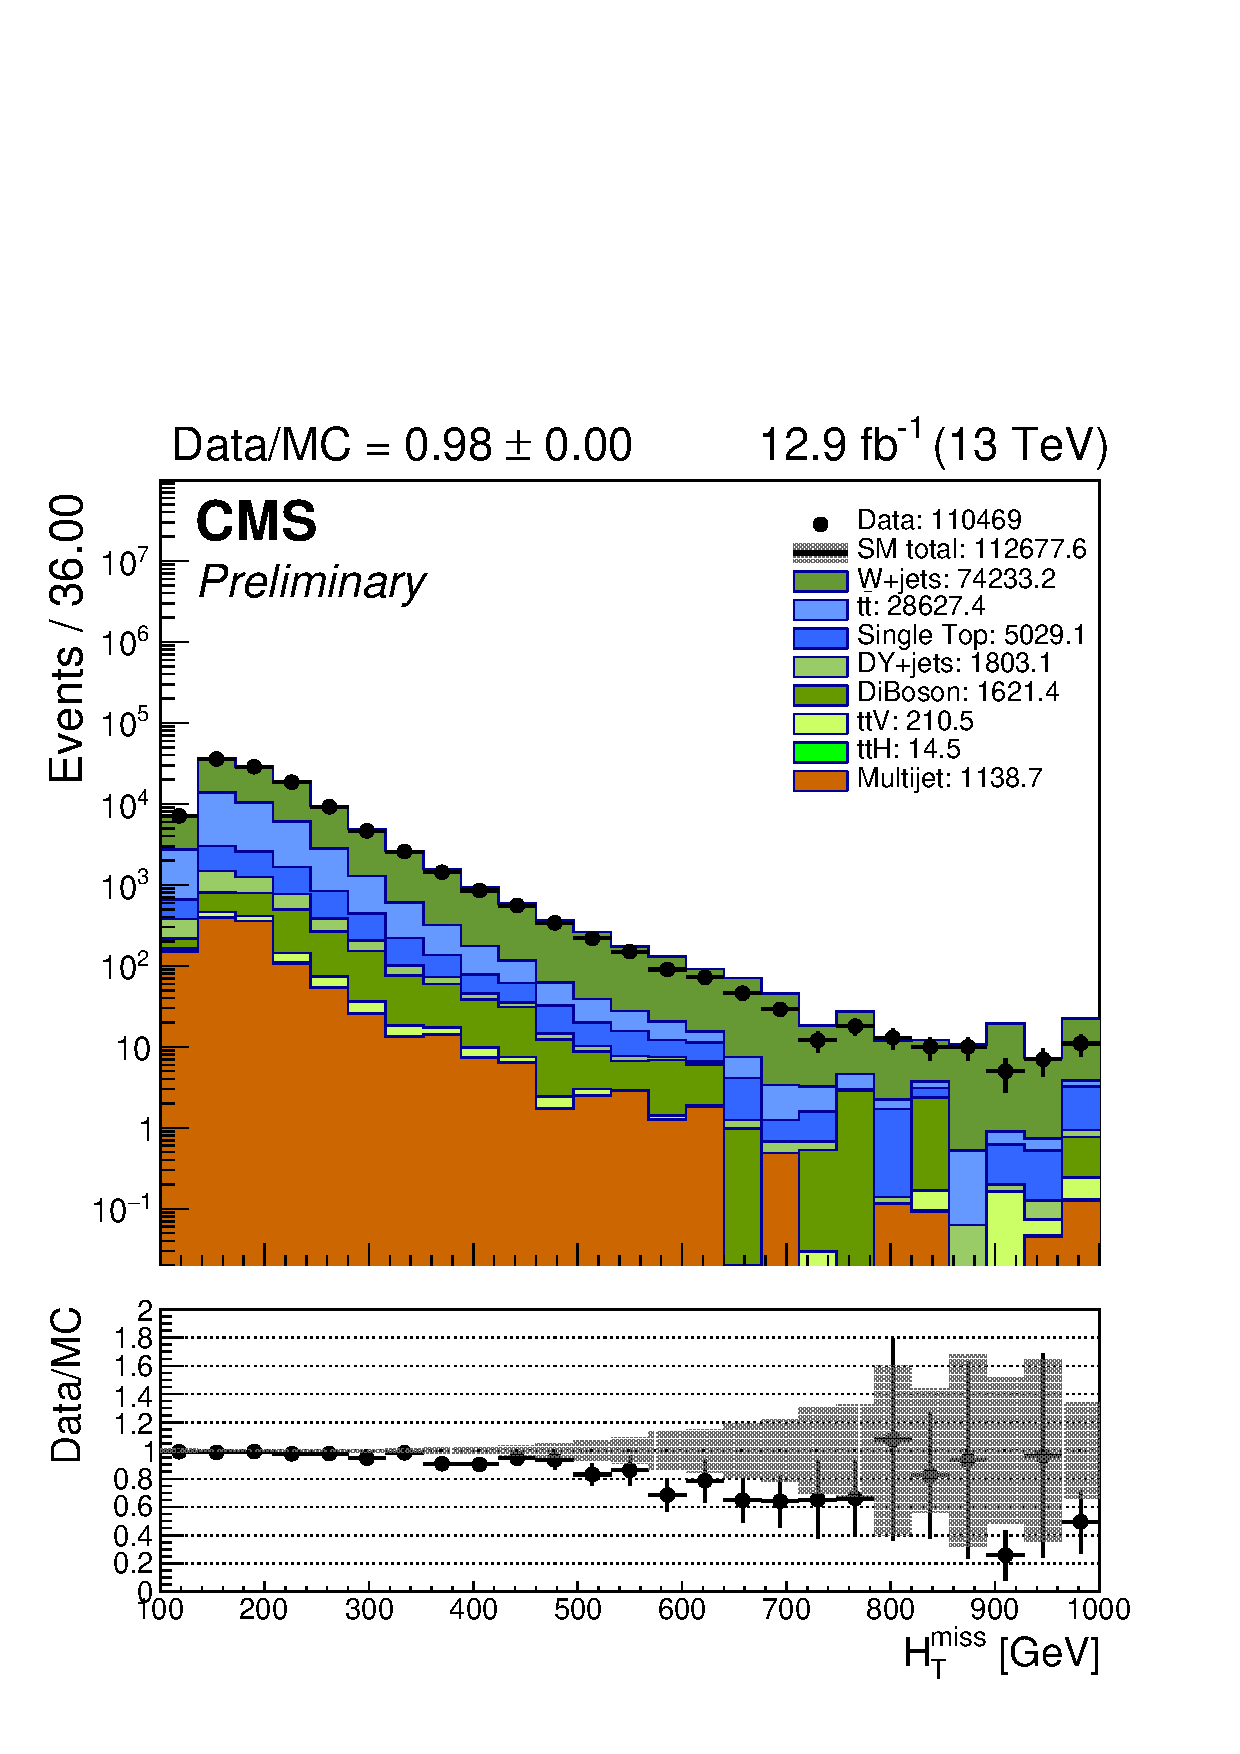
\includegraphics[width=0.5\textwidth]{figs/analysis/distributions/SingleMu/mht40_pt_asym.pdf}} ~~
        \subfloat {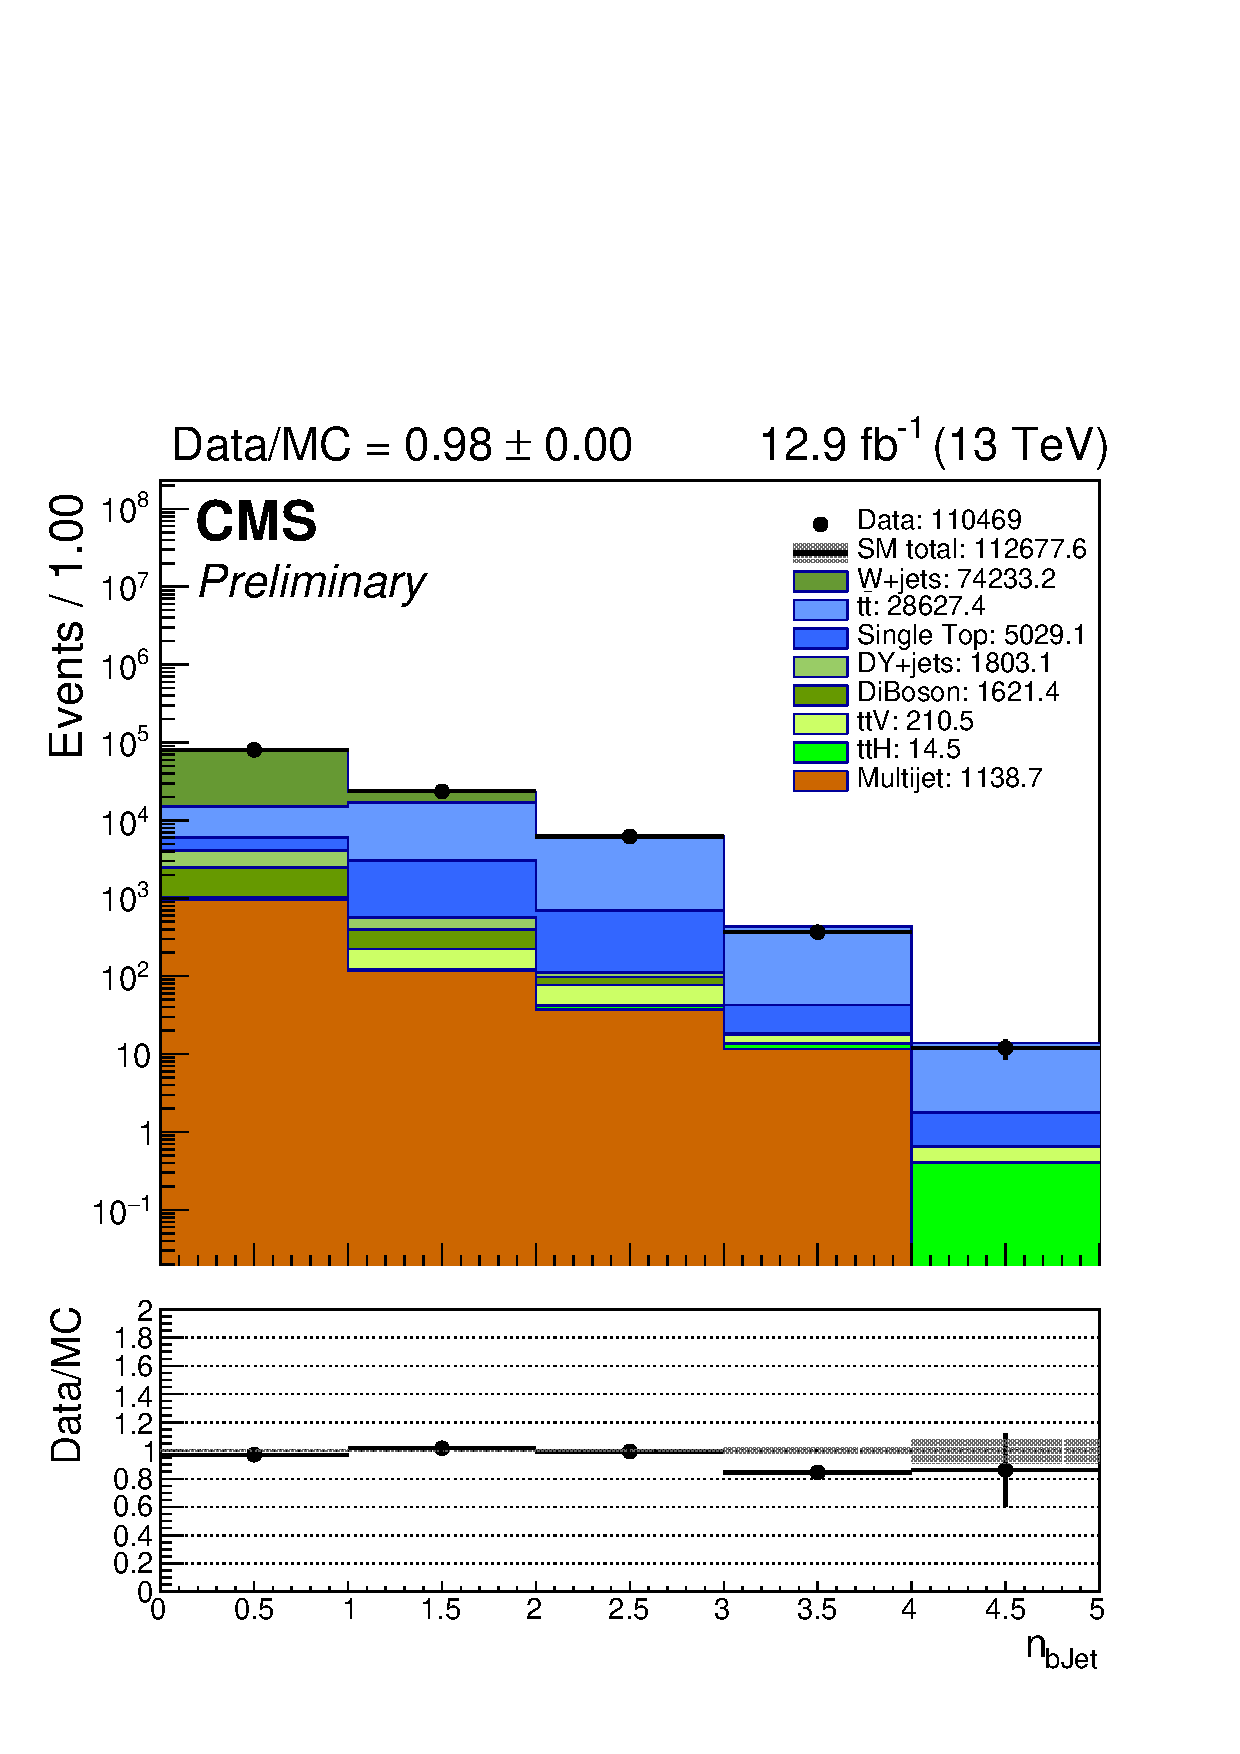
\includegraphics[width=0.5\textwidth]{figs/analysis/distributions/SingleMu/nBJet40_asym.pdf}} \\
        \caption{Key analysis variables for single muon control region (asymmetric \njet bins)}
        \label{fig:distribution_singlemu_asym}
    \end{center}
\end{figure}

\clearpage
\begin{figure}
    \begin{center}        
        \subfloat {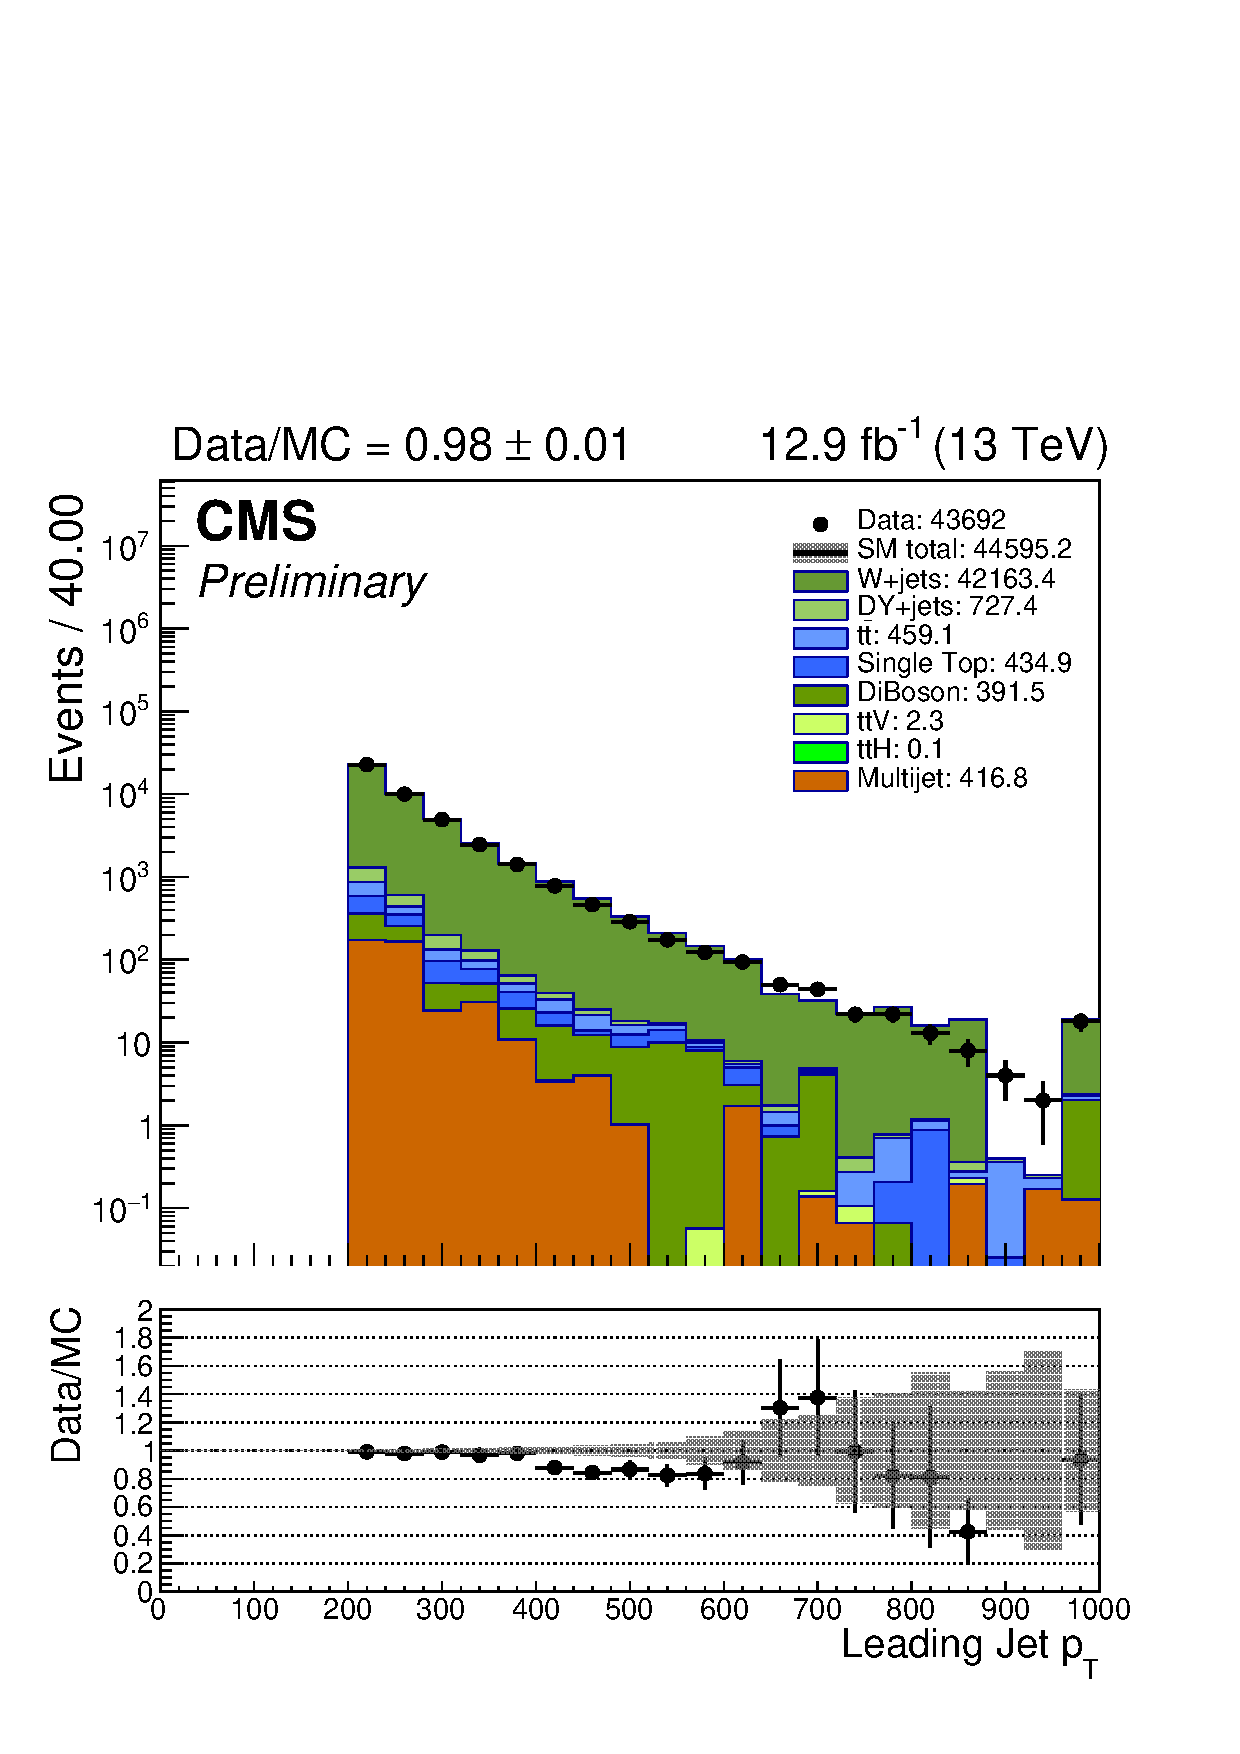
\includegraphics[width=0.5\textwidth]{figs/analysis/distributions/SingleMu/jet_pt[0]_eq1j.pdf}} ~~
        \subfloat {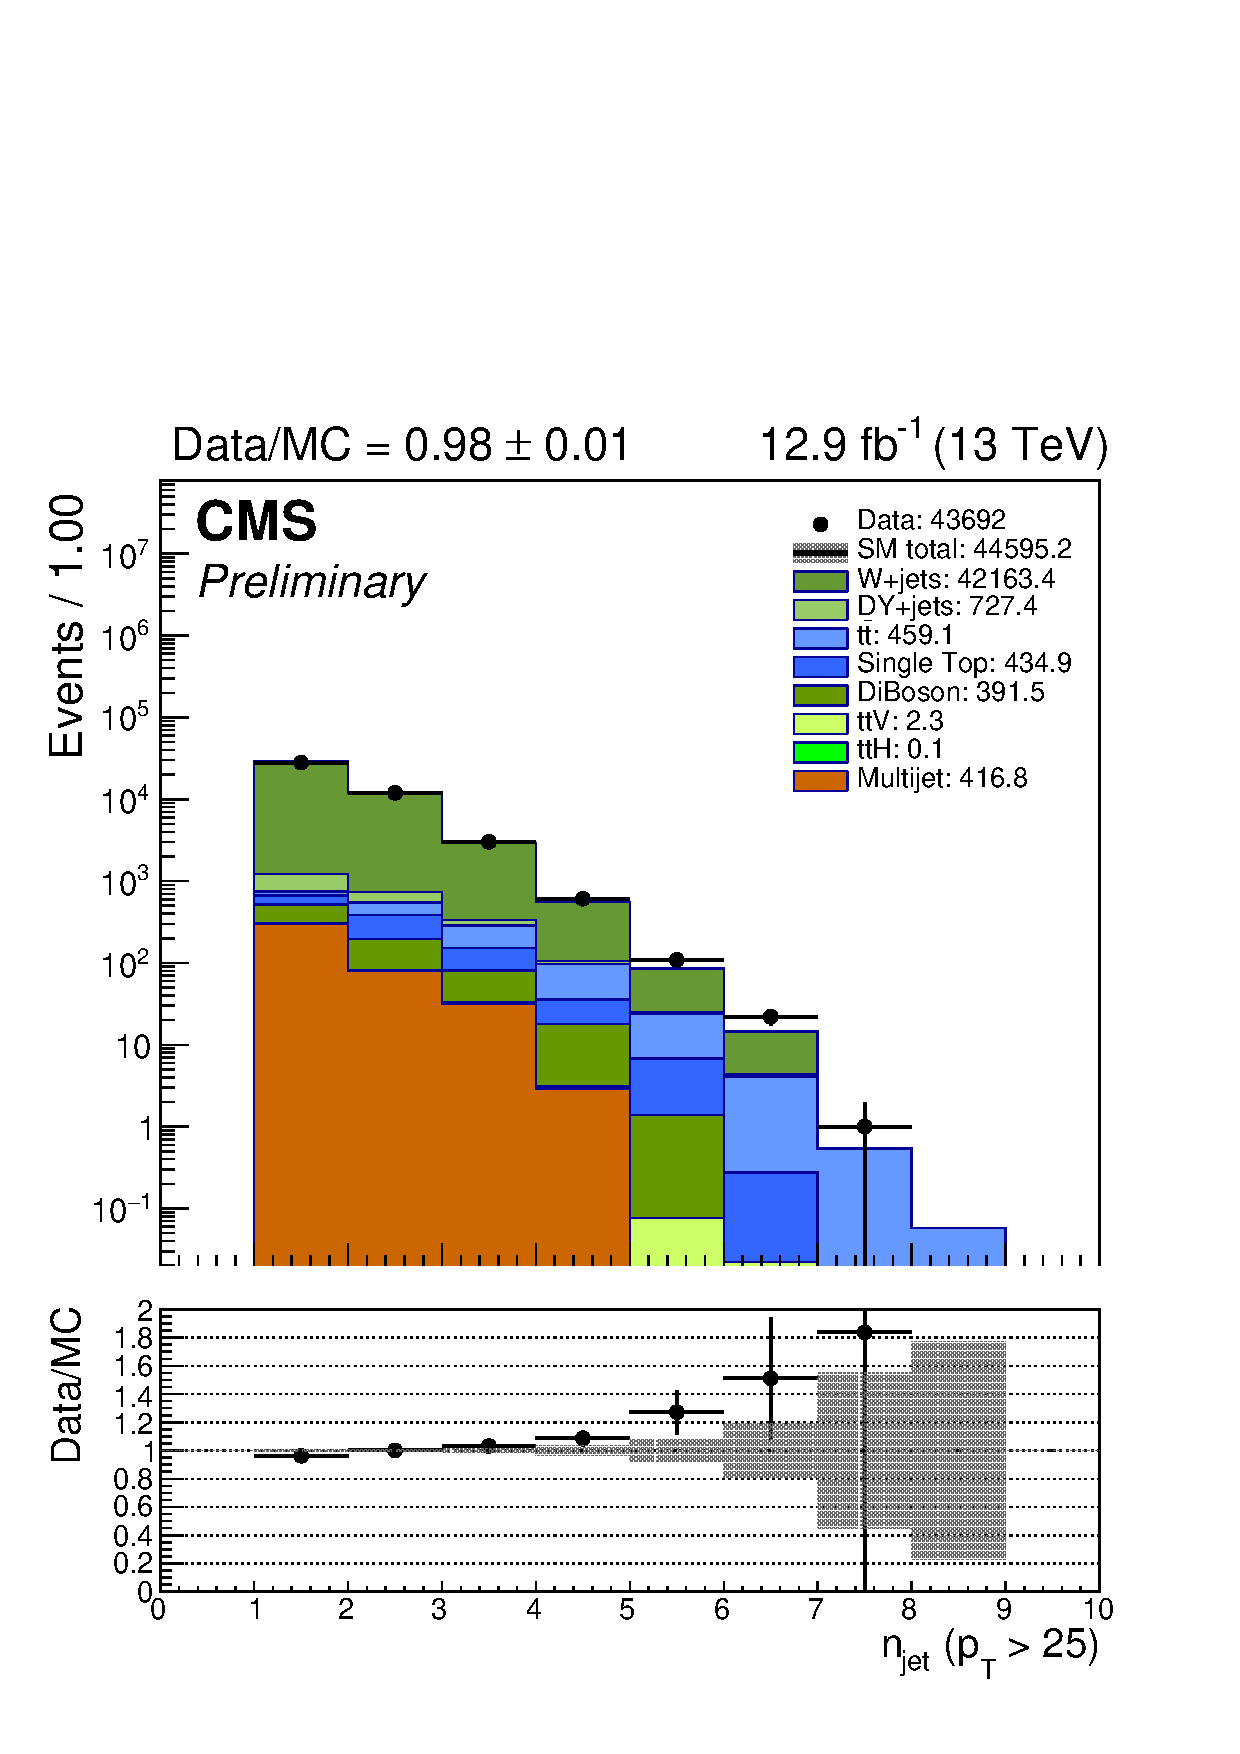
\includegraphics[width=0.5\textwidth]{figs/analysis/distributions/SingleMu/njetInc_eq1j.pdf}} \\
        \subfloat {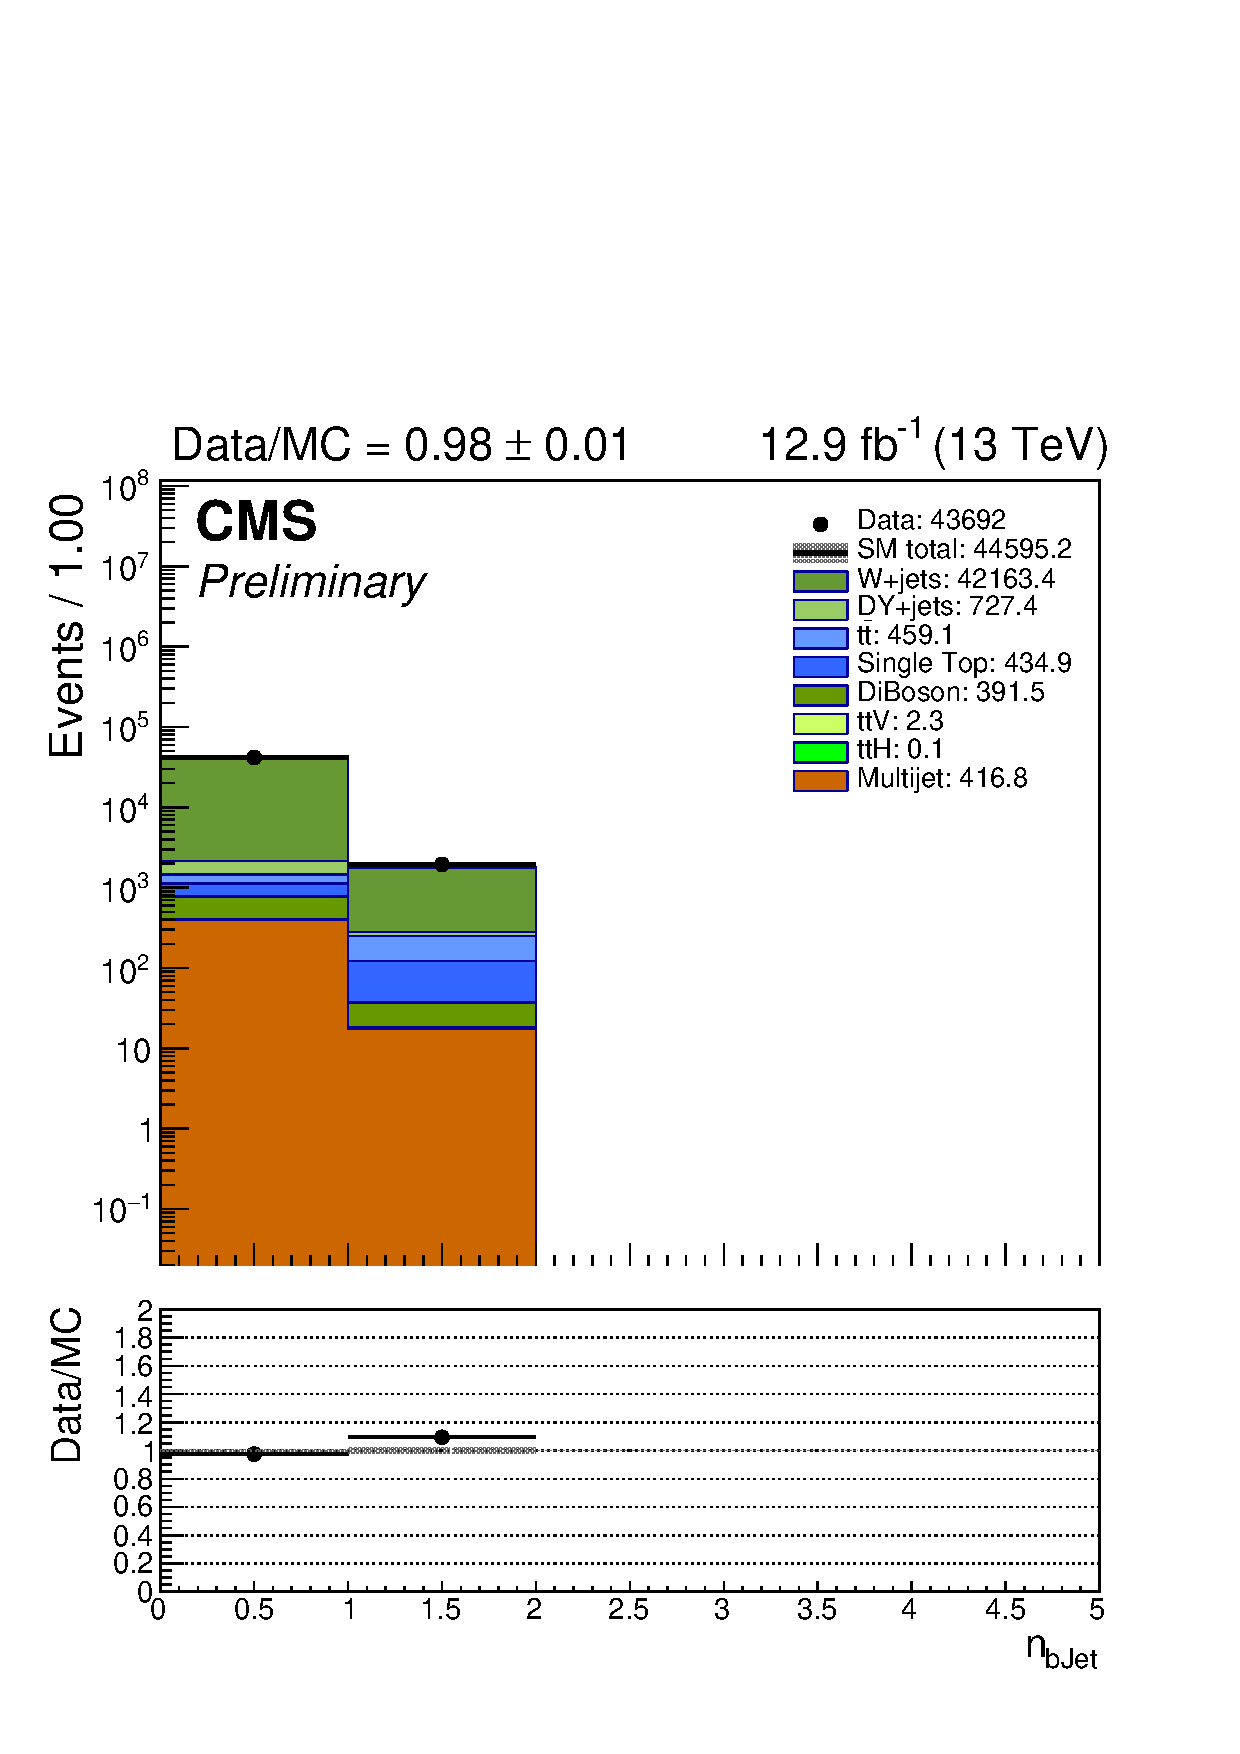
\includegraphics[width=0.5\textwidth]{figs/analysis/distributions/SingleMu/nBJet40_eq1j.pdf}} ~~
        \subfloat {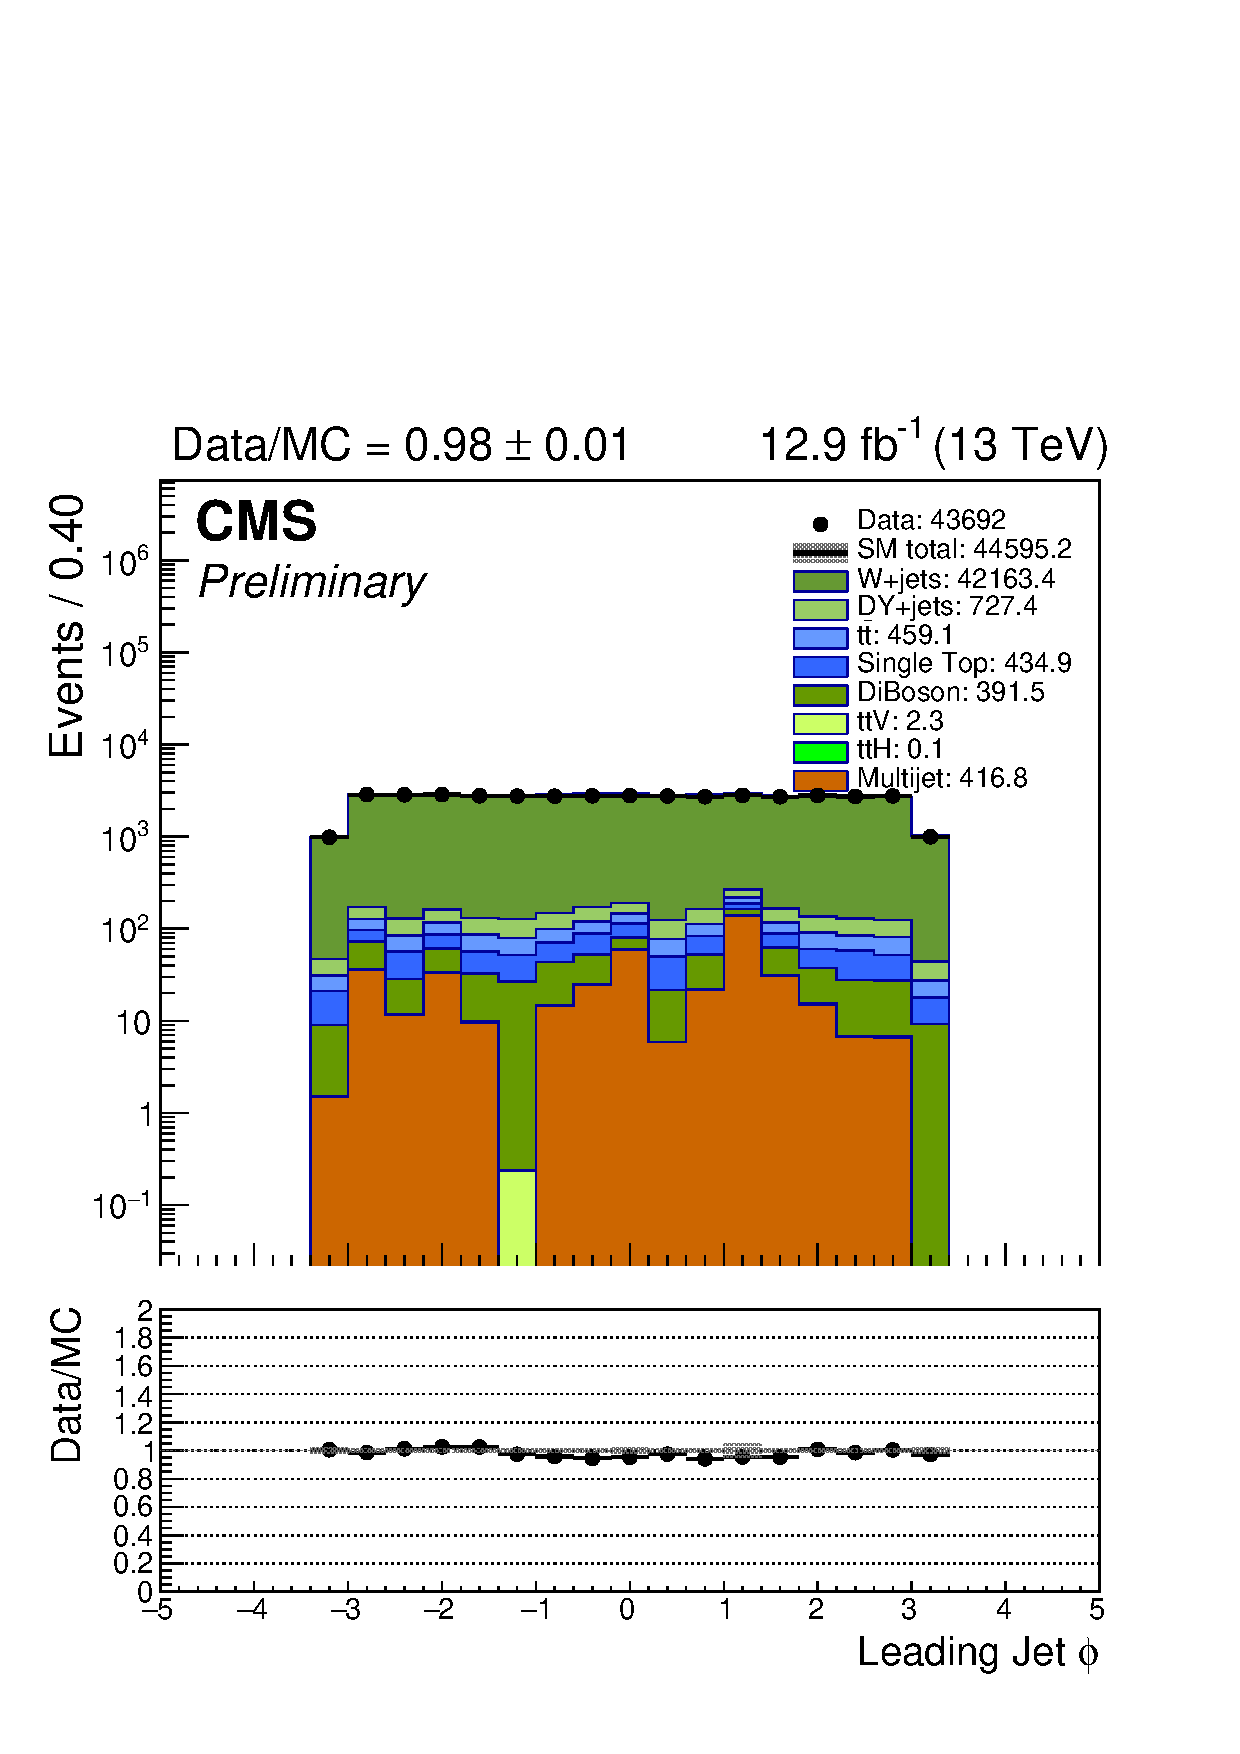
\includegraphics[width=0.5\textwidth]{figs/analysis/distributions/SingleMu/jet_phi[0]_eq1j.pdf}} \\
        \caption{Key analysis variables for single muon control region (monojet bins)}
        \label{fig:distribution_singlemu_mono}
    \end{center}
\end{figure}

% \clearpage
% \subsection{Yields and distributions for the di-muon + jets control sample}

\begin{figure}
    \begin{center}
        \subfloat {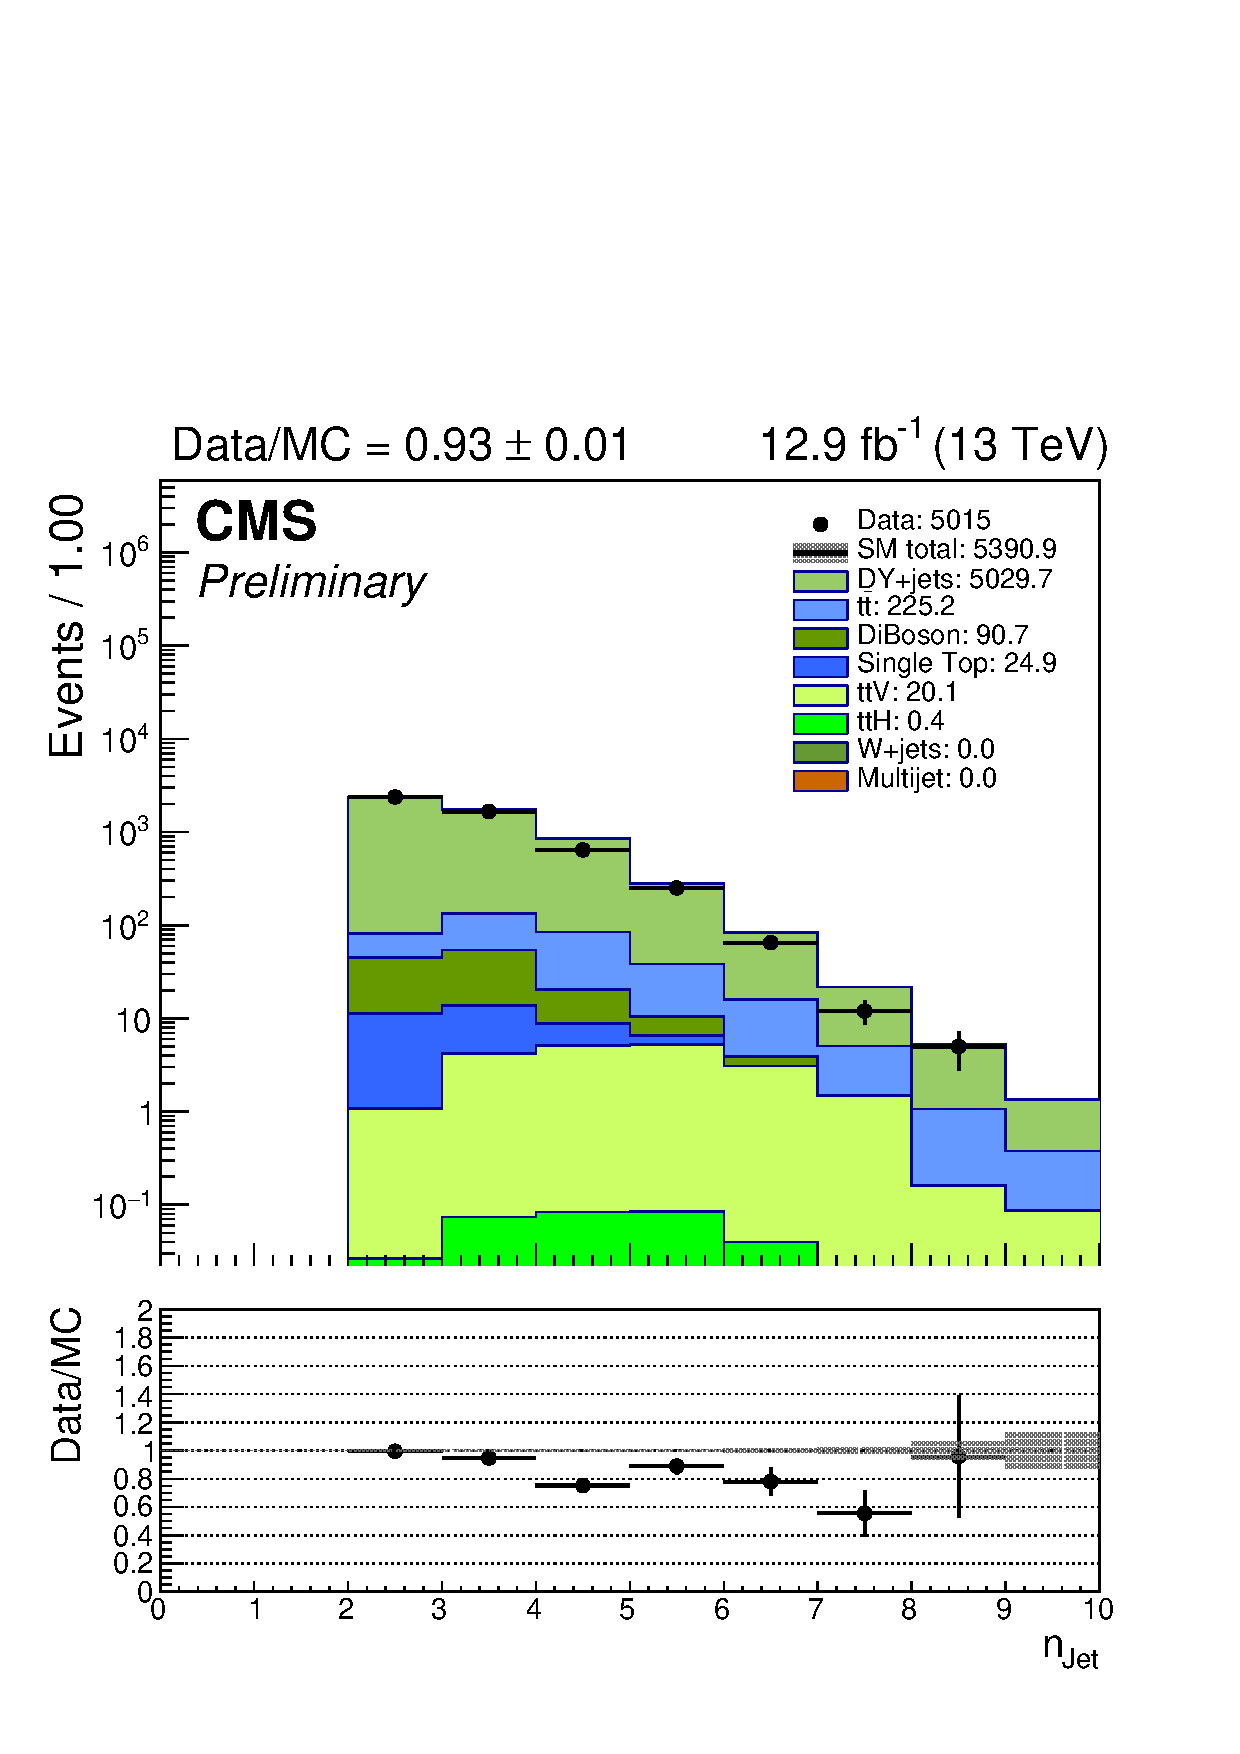
\includegraphics[width=0.5\textwidth]{figs/analysis/distributions/DoubleMu/nJet40_sym.pdf}} ~~
        \subfloat {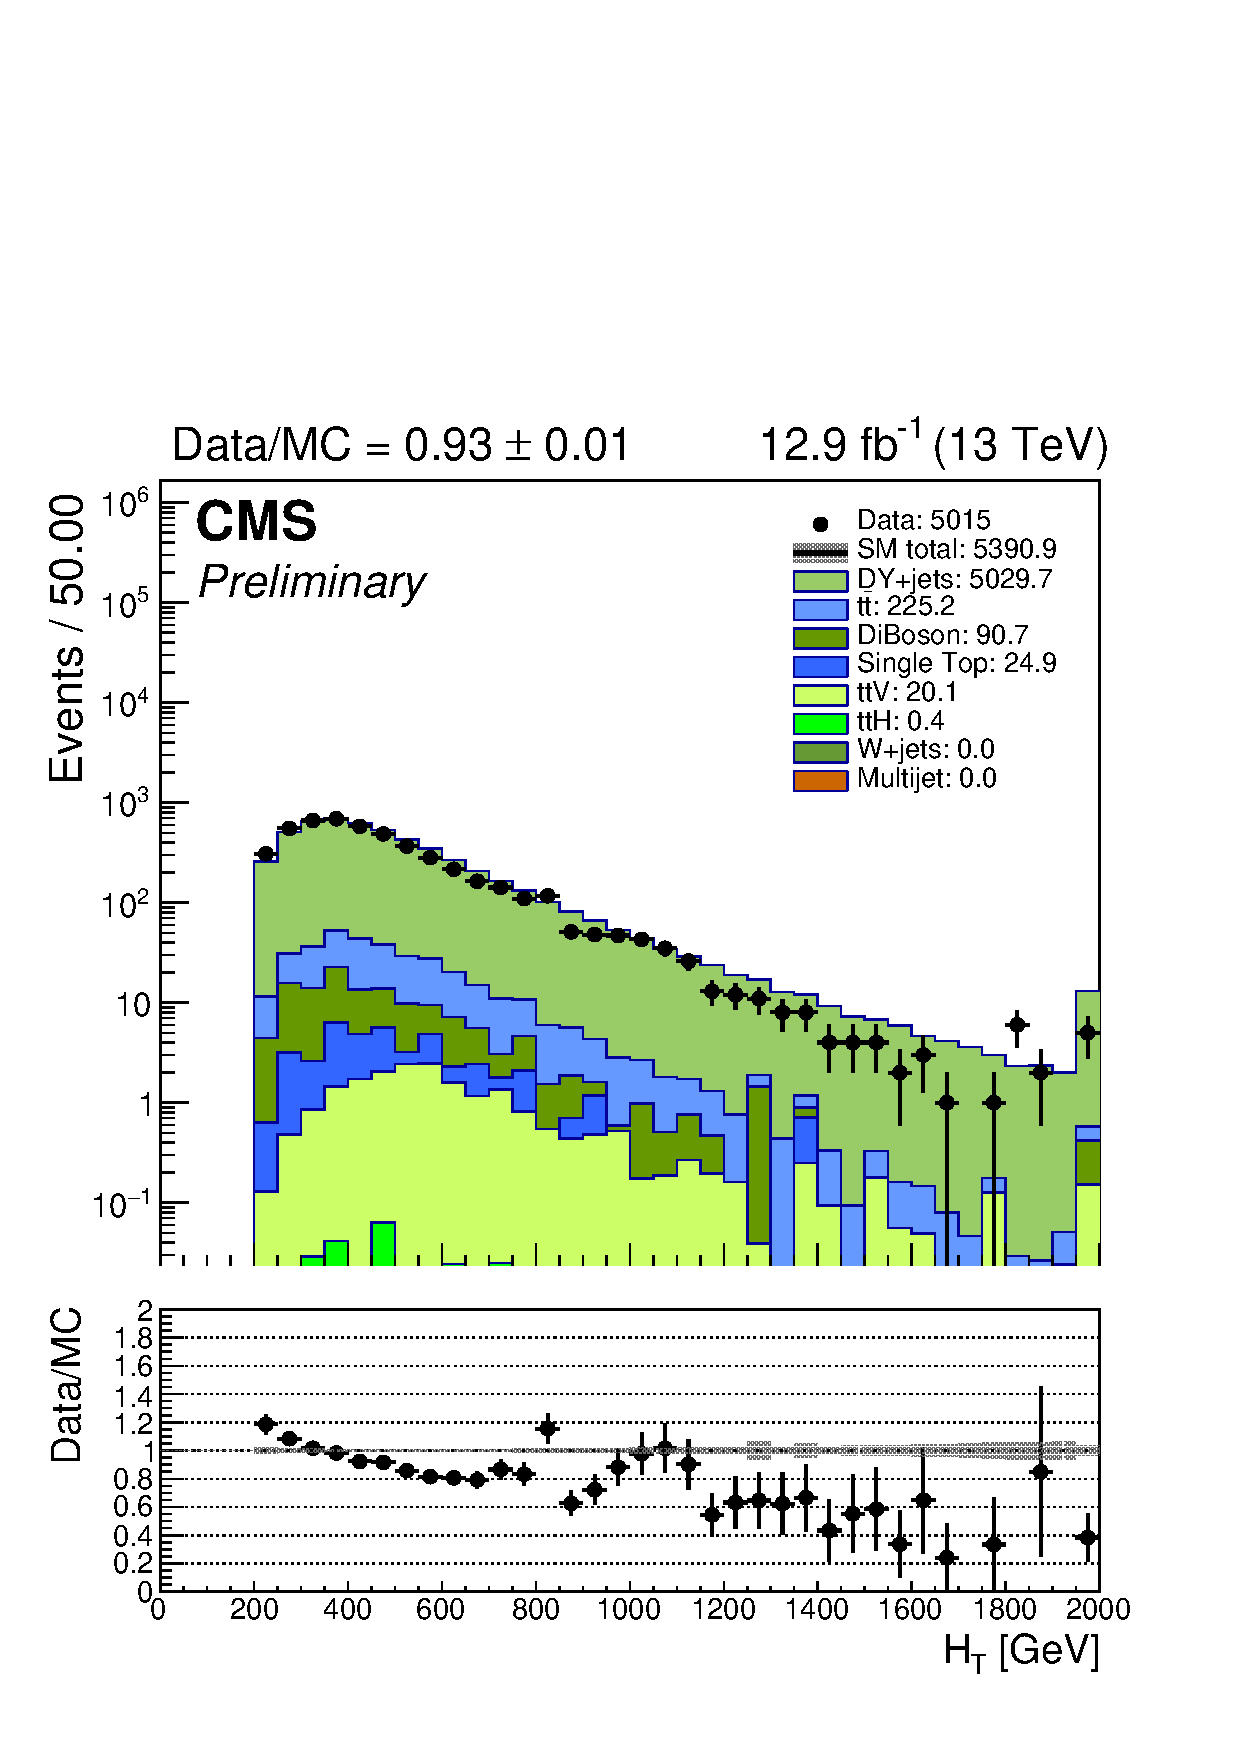
\includegraphics[width=0.5\textwidth]{figs/analysis/distributions/DoubleMu/ht40_sym.pdf}} \\
        \subfloat {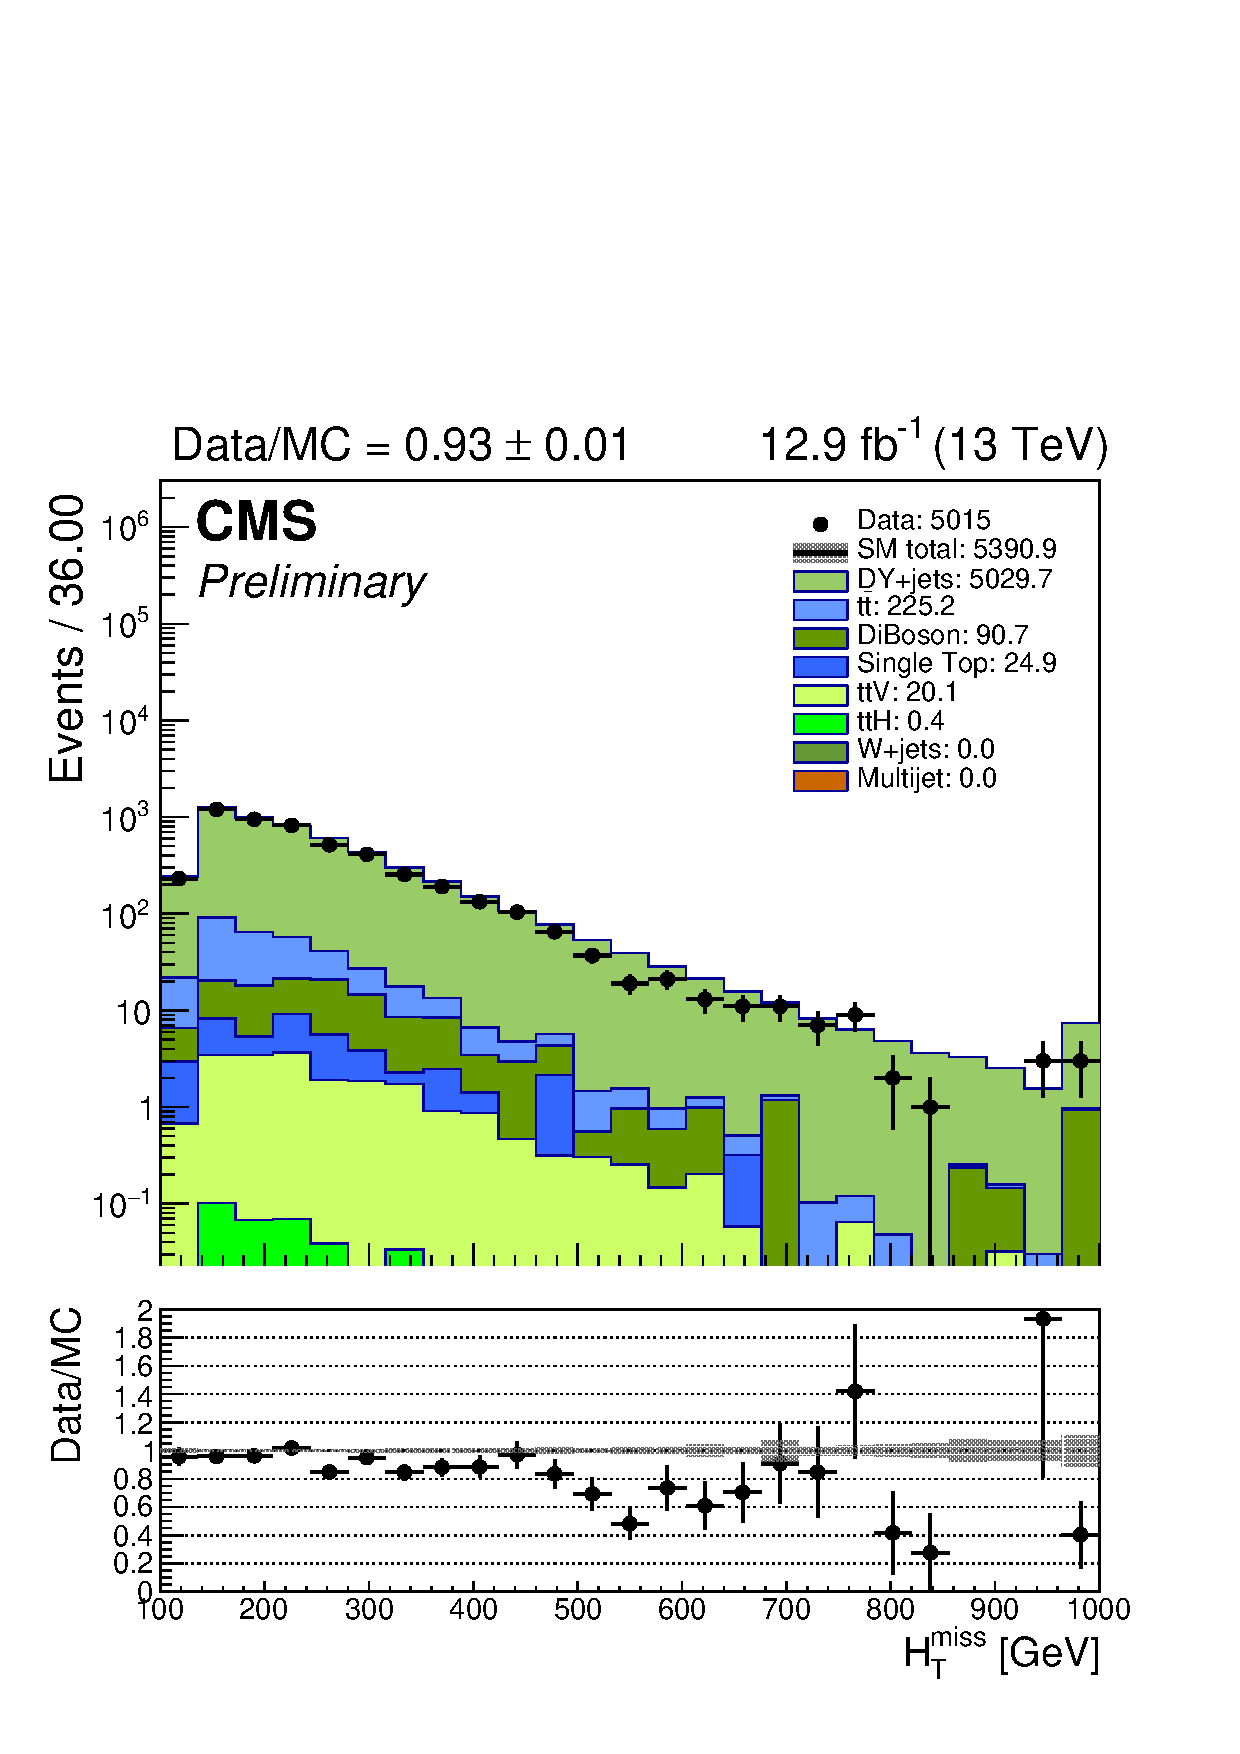
\includegraphics[width=0.5\textwidth]{figs/analysis/distributions/DoubleMu/mht40_pt_sym.pdf}} ~~
        \subfloat {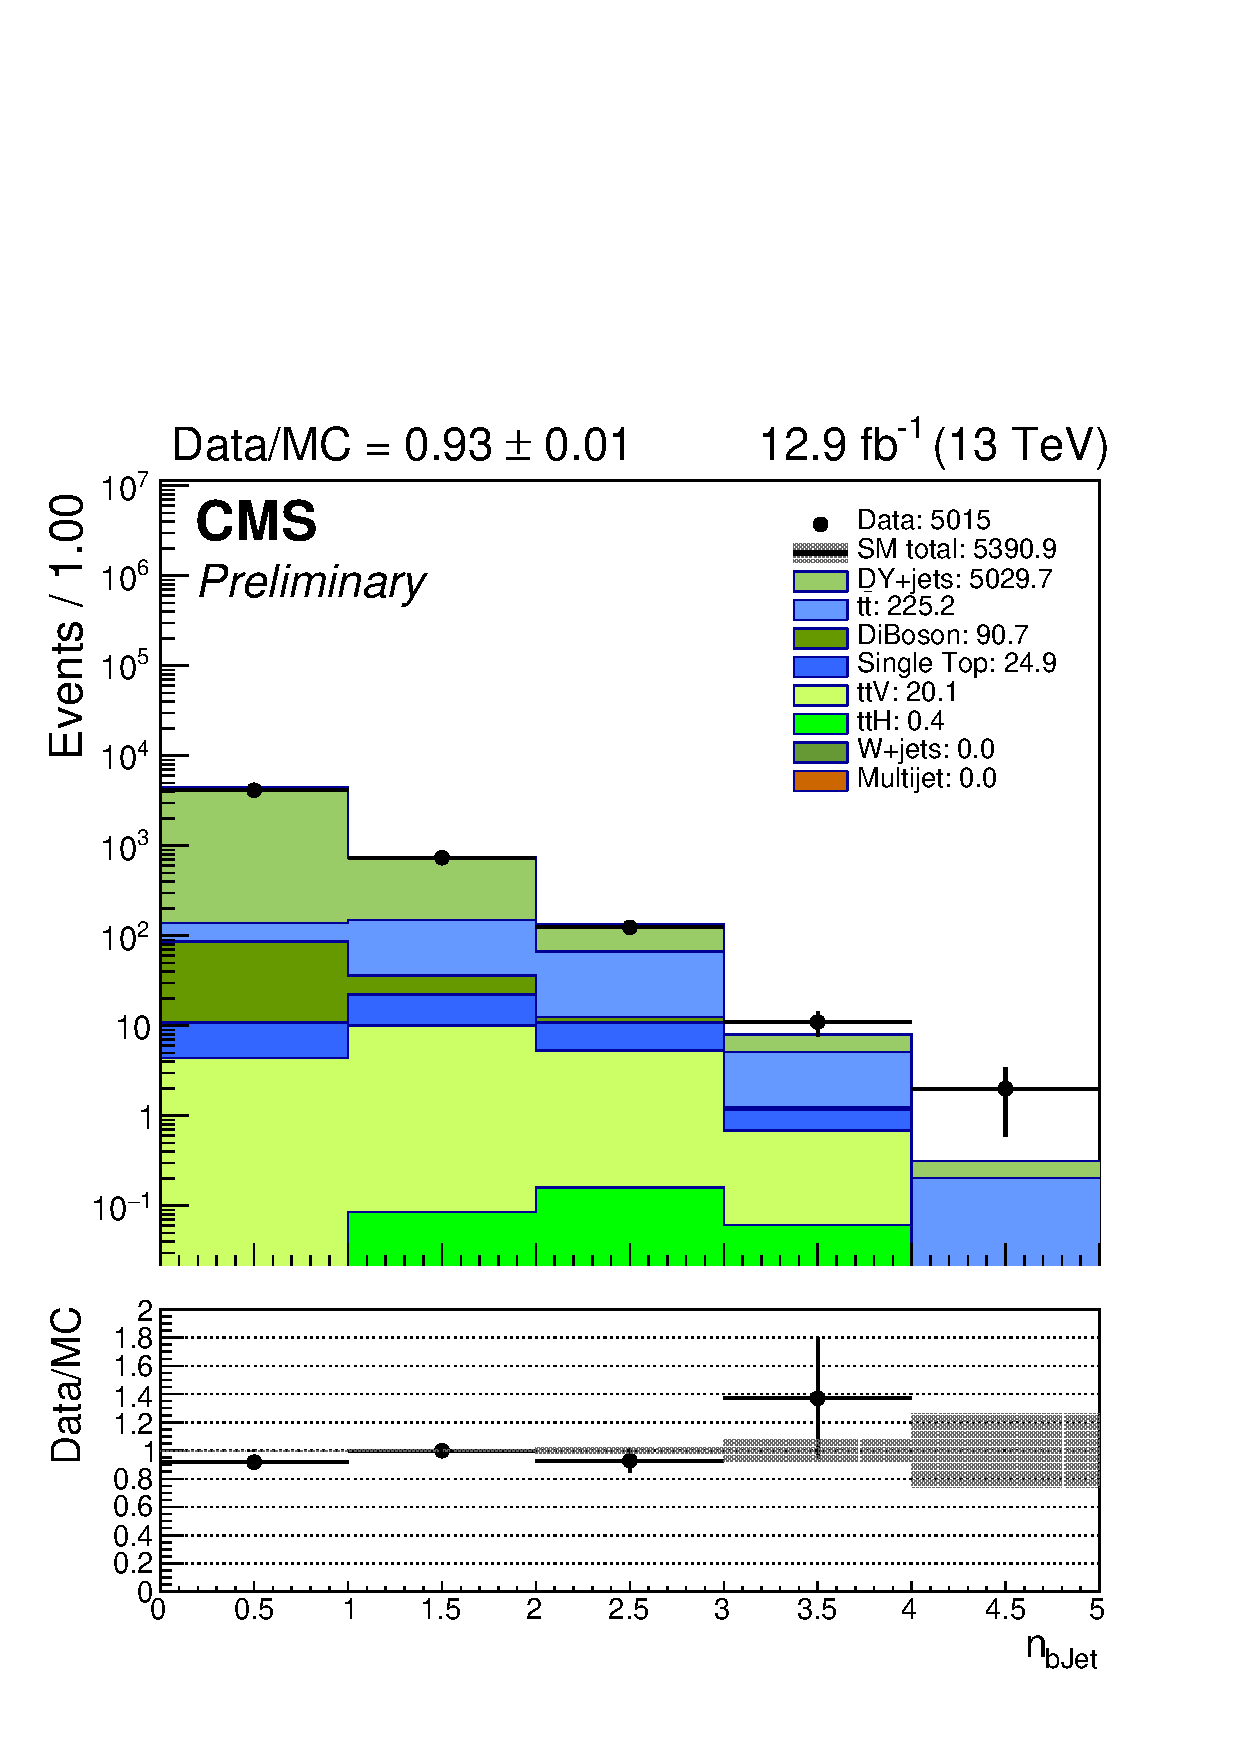
\includegraphics[width=0.5\textwidth]{figs/analysis/distributions/DoubleMu/nBJet40_sym.pdf}} \\
        \caption{Key analysis variables for double muon control region (symmetric \njet bins)}
        \label{fig:distribution_doublemu_sym}
    \end{center}
\end{figure}

\clearpage
\begin{figure}
    \begin{center}
        \subfloat {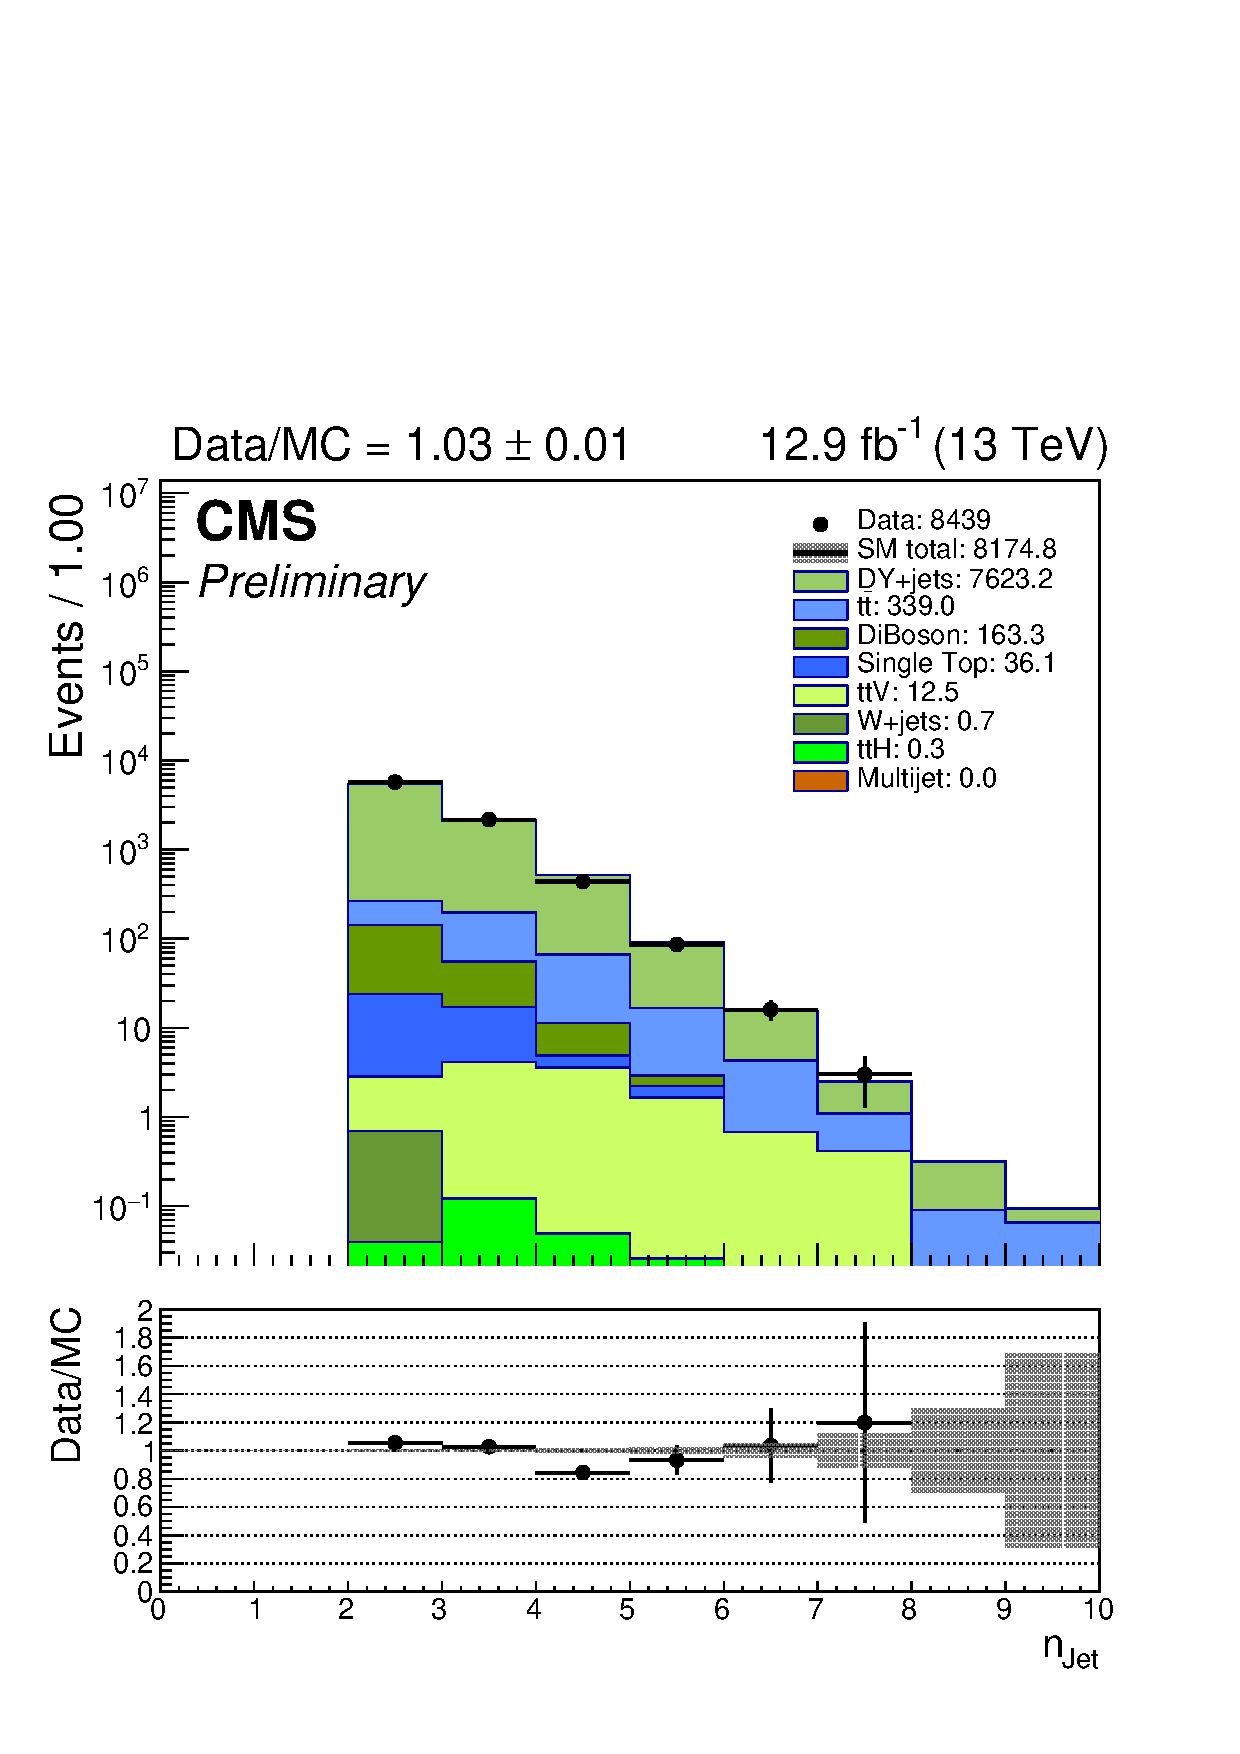
\includegraphics[width=0.5\textwidth]{figs/analysis/distributions/DoubleMu/nJet40_asym.pdf}} ~~
        \subfloat {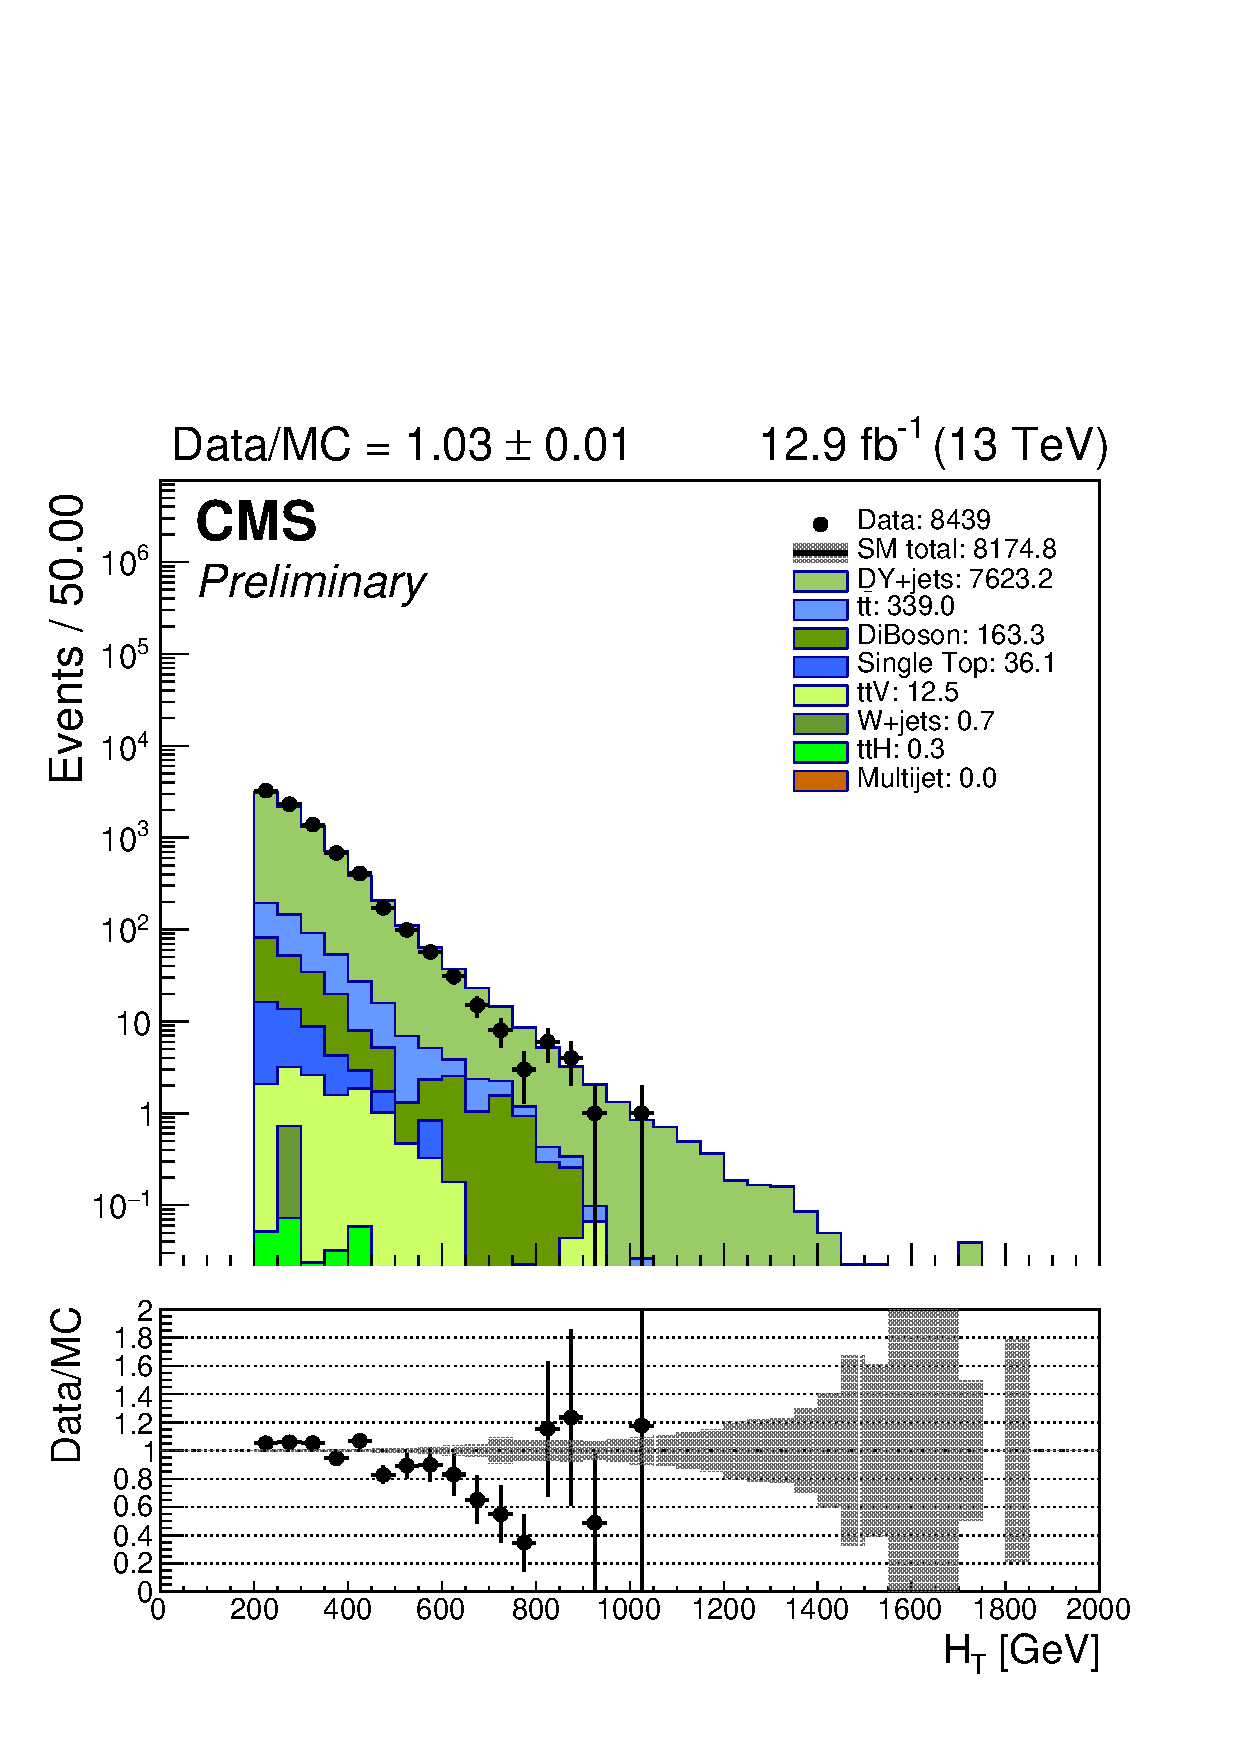
\includegraphics[width=0.5\textwidth]{figs/analysis/distributions/DoubleMu/ht40_asym.pdf}} \\
        \subfloat {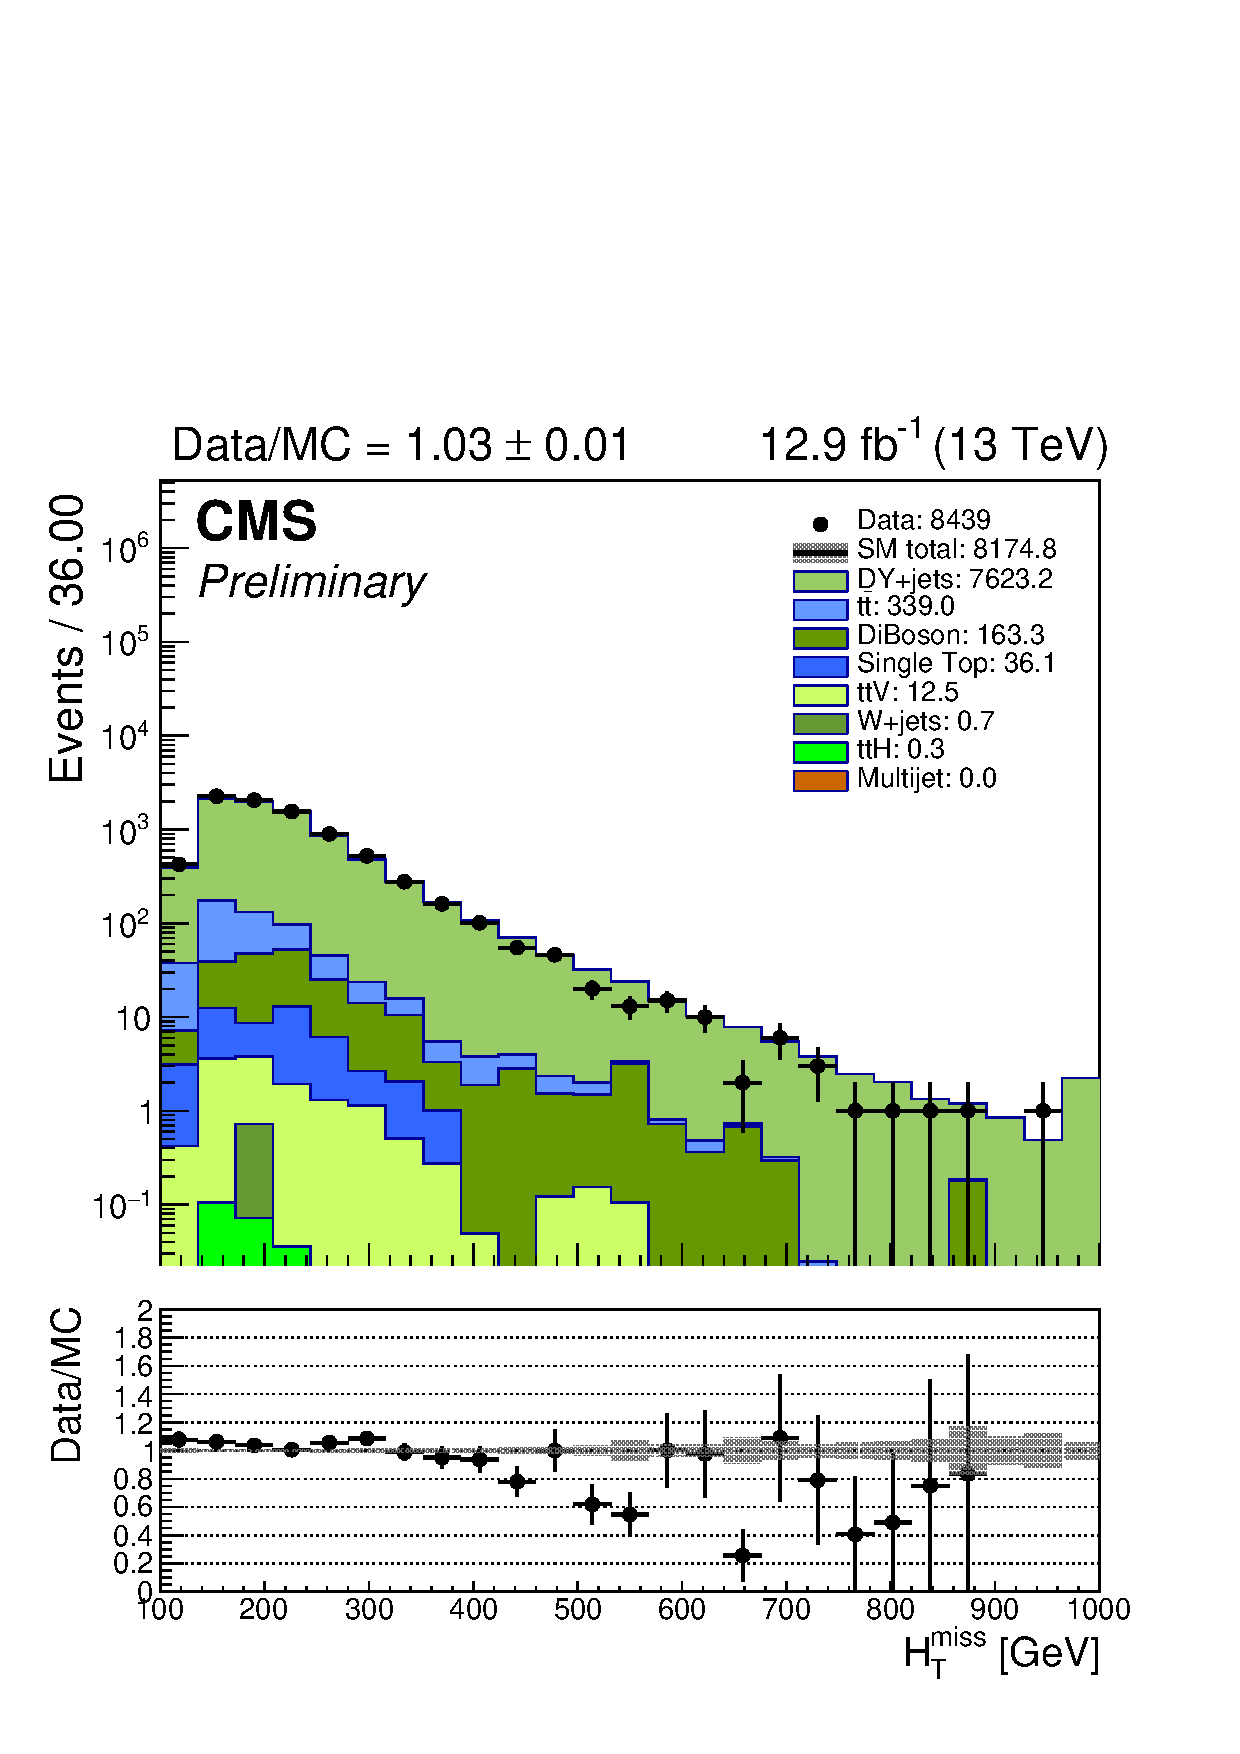
\includegraphics[width=0.5\textwidth]{figs/analysis/distributions/DoubleMu/mht40_pt_asym.pdf}} ~~
        \subfloat {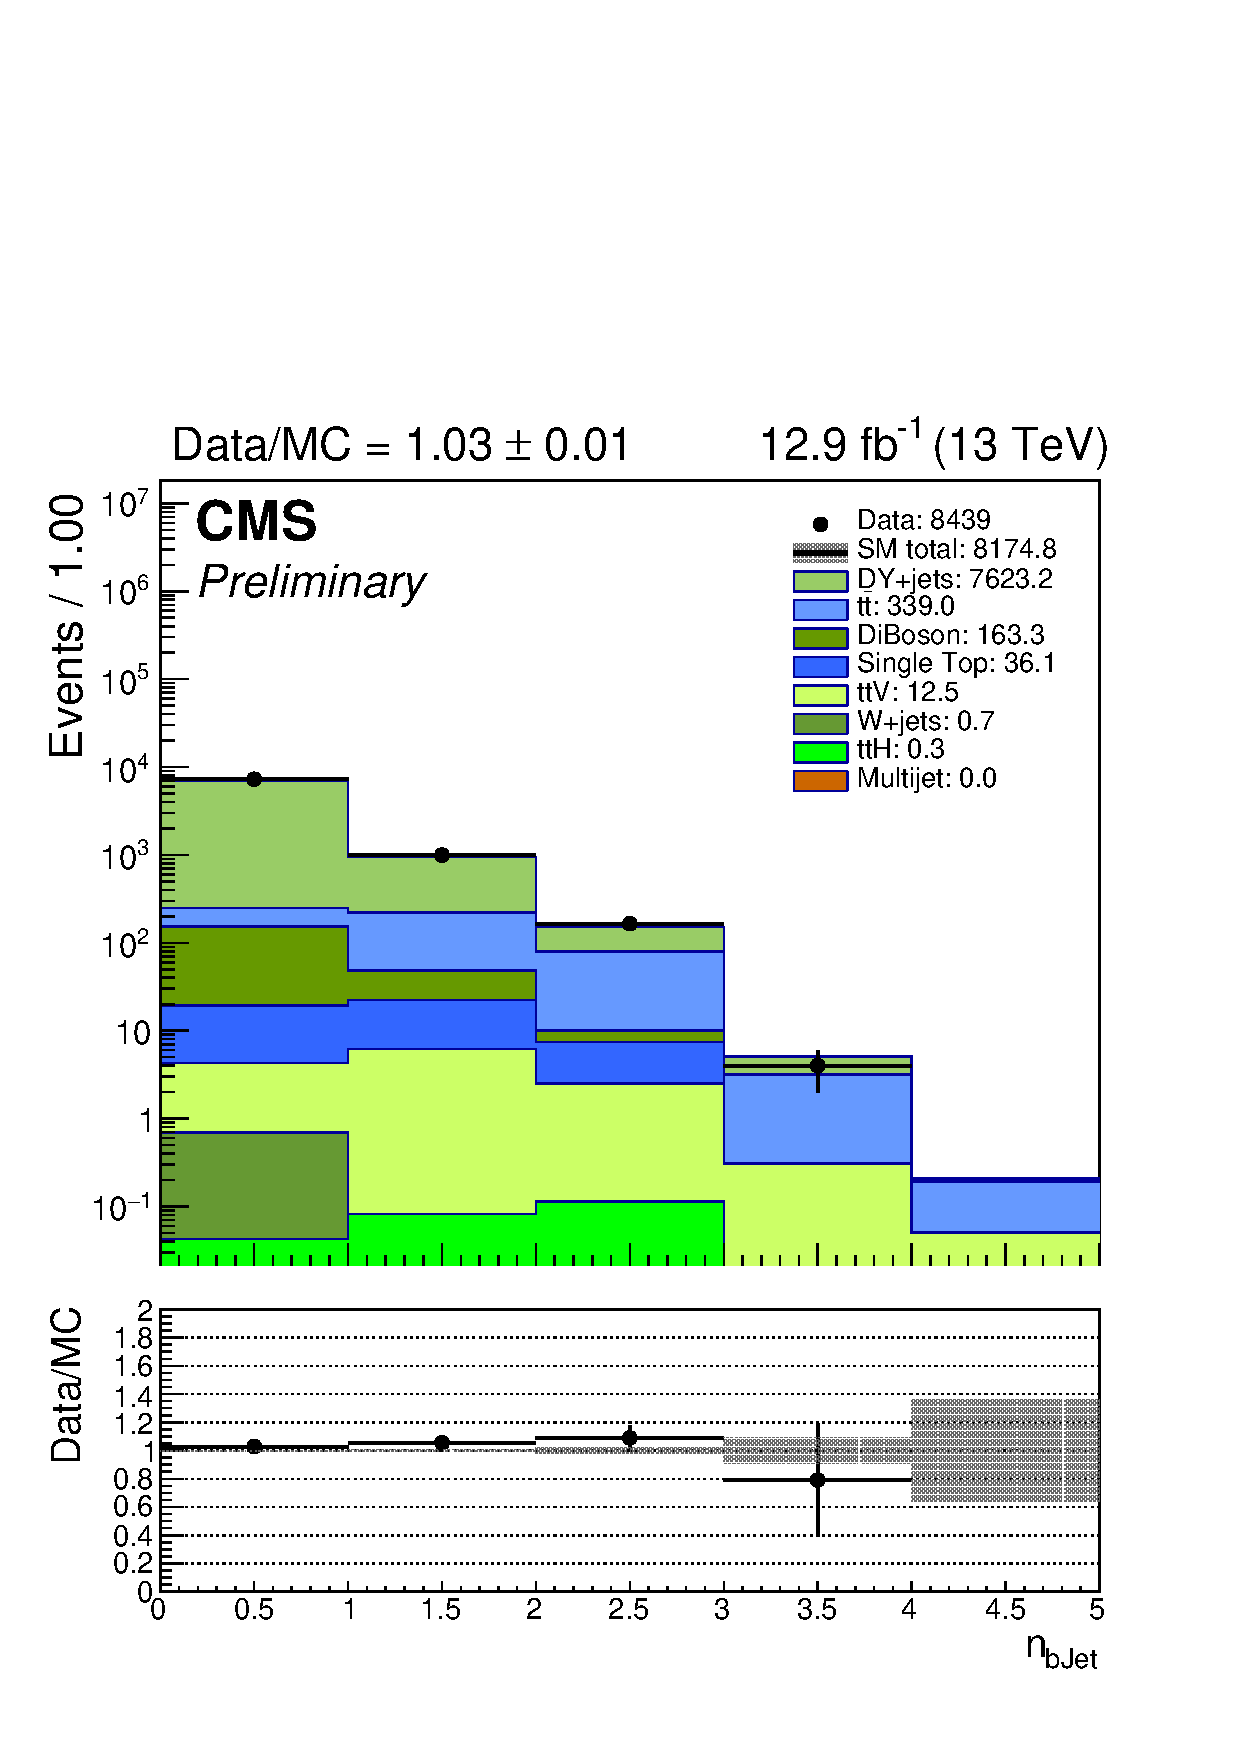
\includegraphics[width=0.5\textwidth]{figs/analysis/distributions/DoubleMu/nBJet40_asym.pdf}} \\
        \caption{Key analysis variables for double muon control region (asymmetric \njet bins)}
        \label{fig:distribution_doublemu_asym}
    \end{center}
\end{figure}

\begin{figure}
    \begin{center} 
        \subfloat {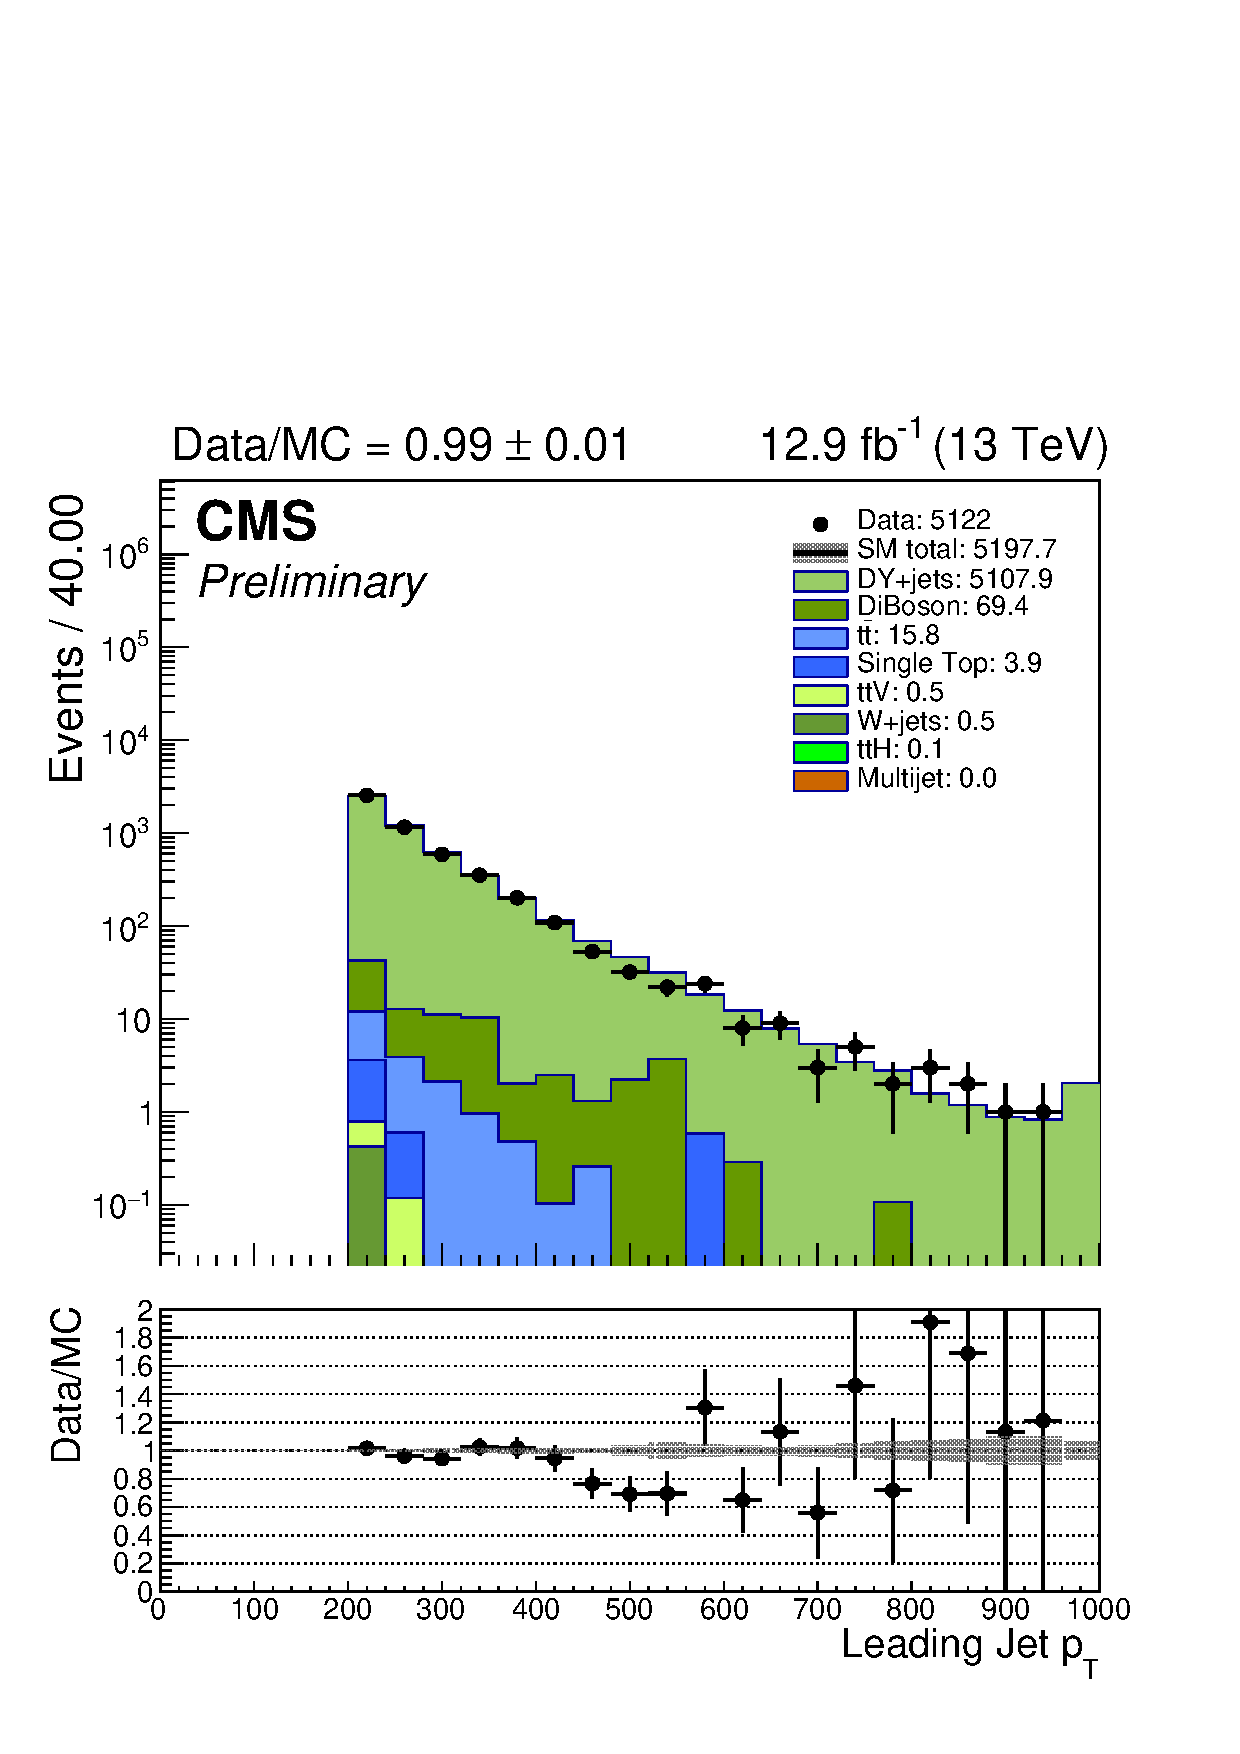
\includegraphics[width=0.5\textwidth]{figs/analysis/distributions/DoubleMu/jet_pt[0]_eq1j.pdf}} ~~
        \subfloat {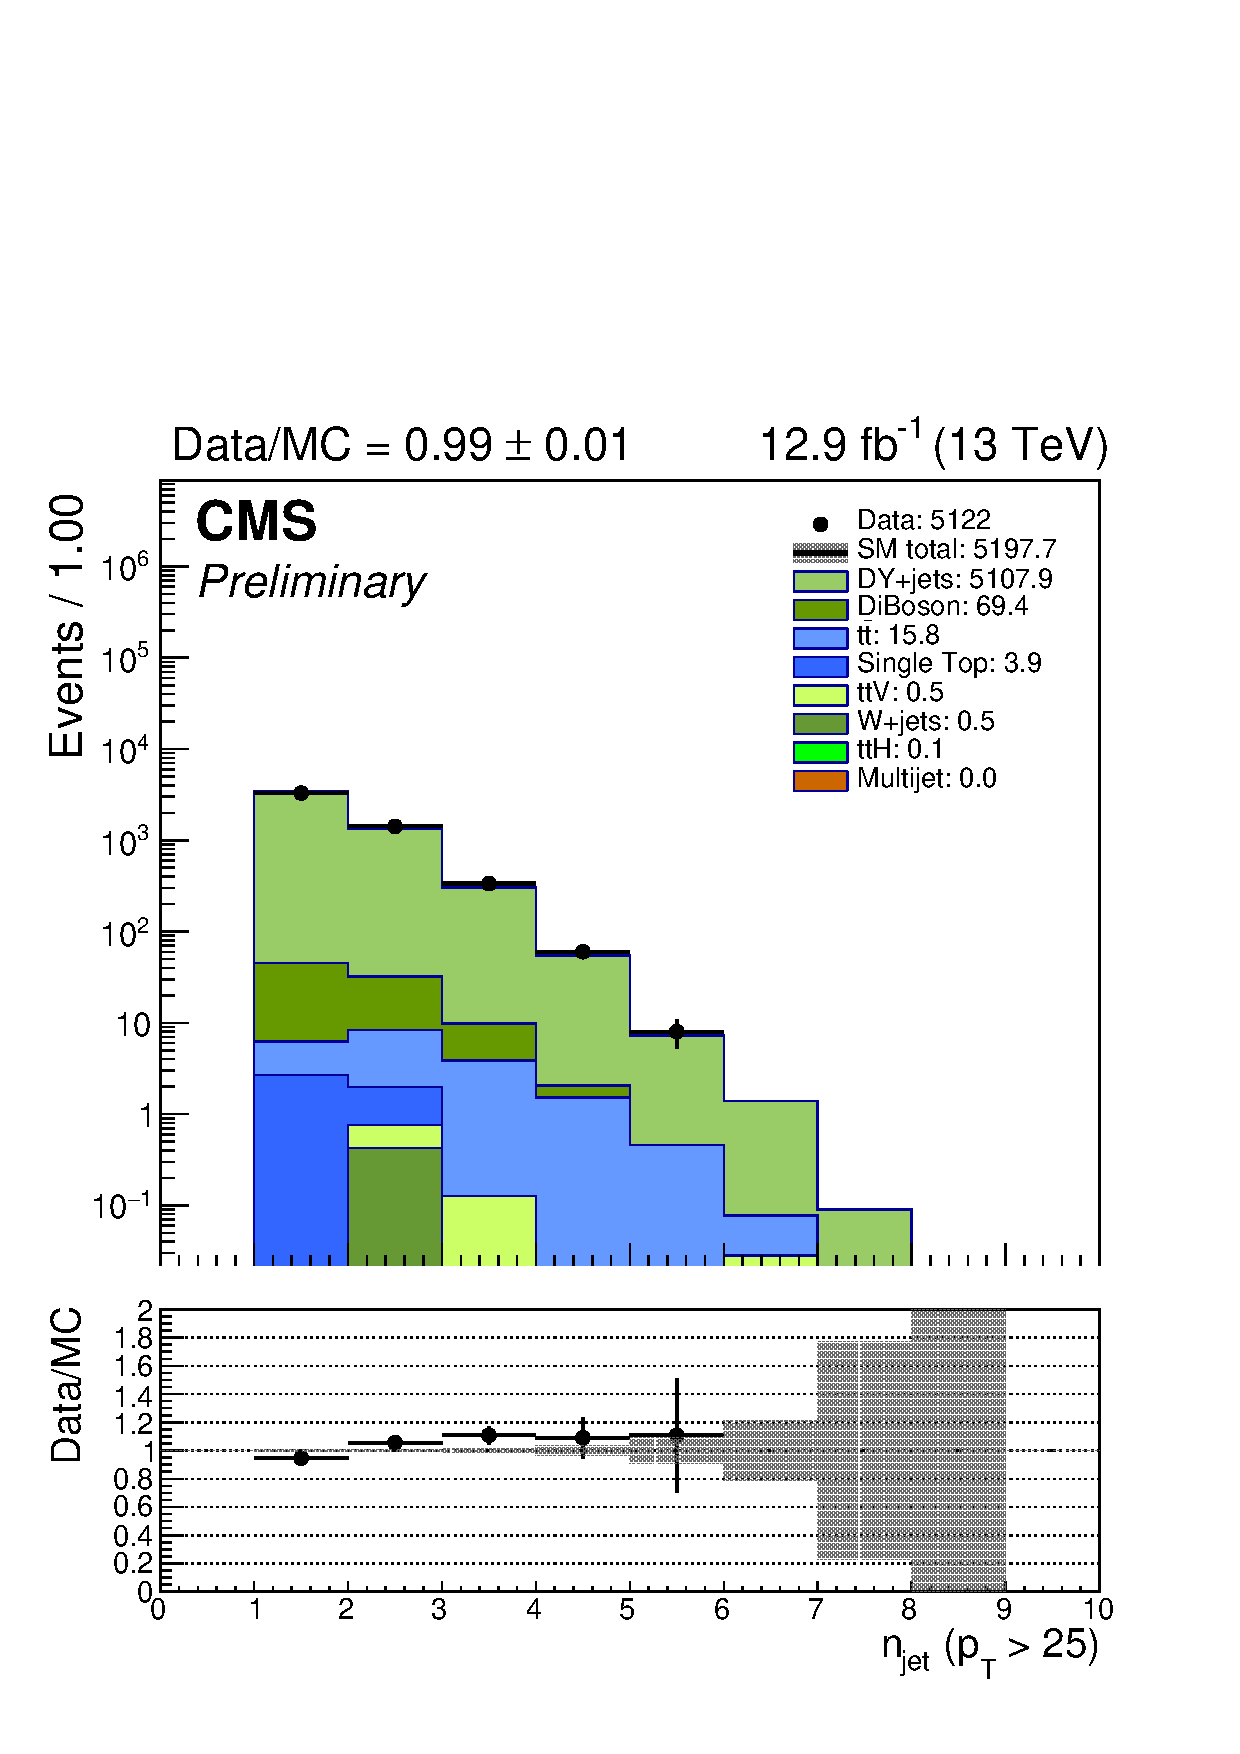
\includegraphics[width=0.5\textwidth]{figs/analysis/distributions/DoubleMu/njetInc_eq1j.pdf}} \\
        \subfloat {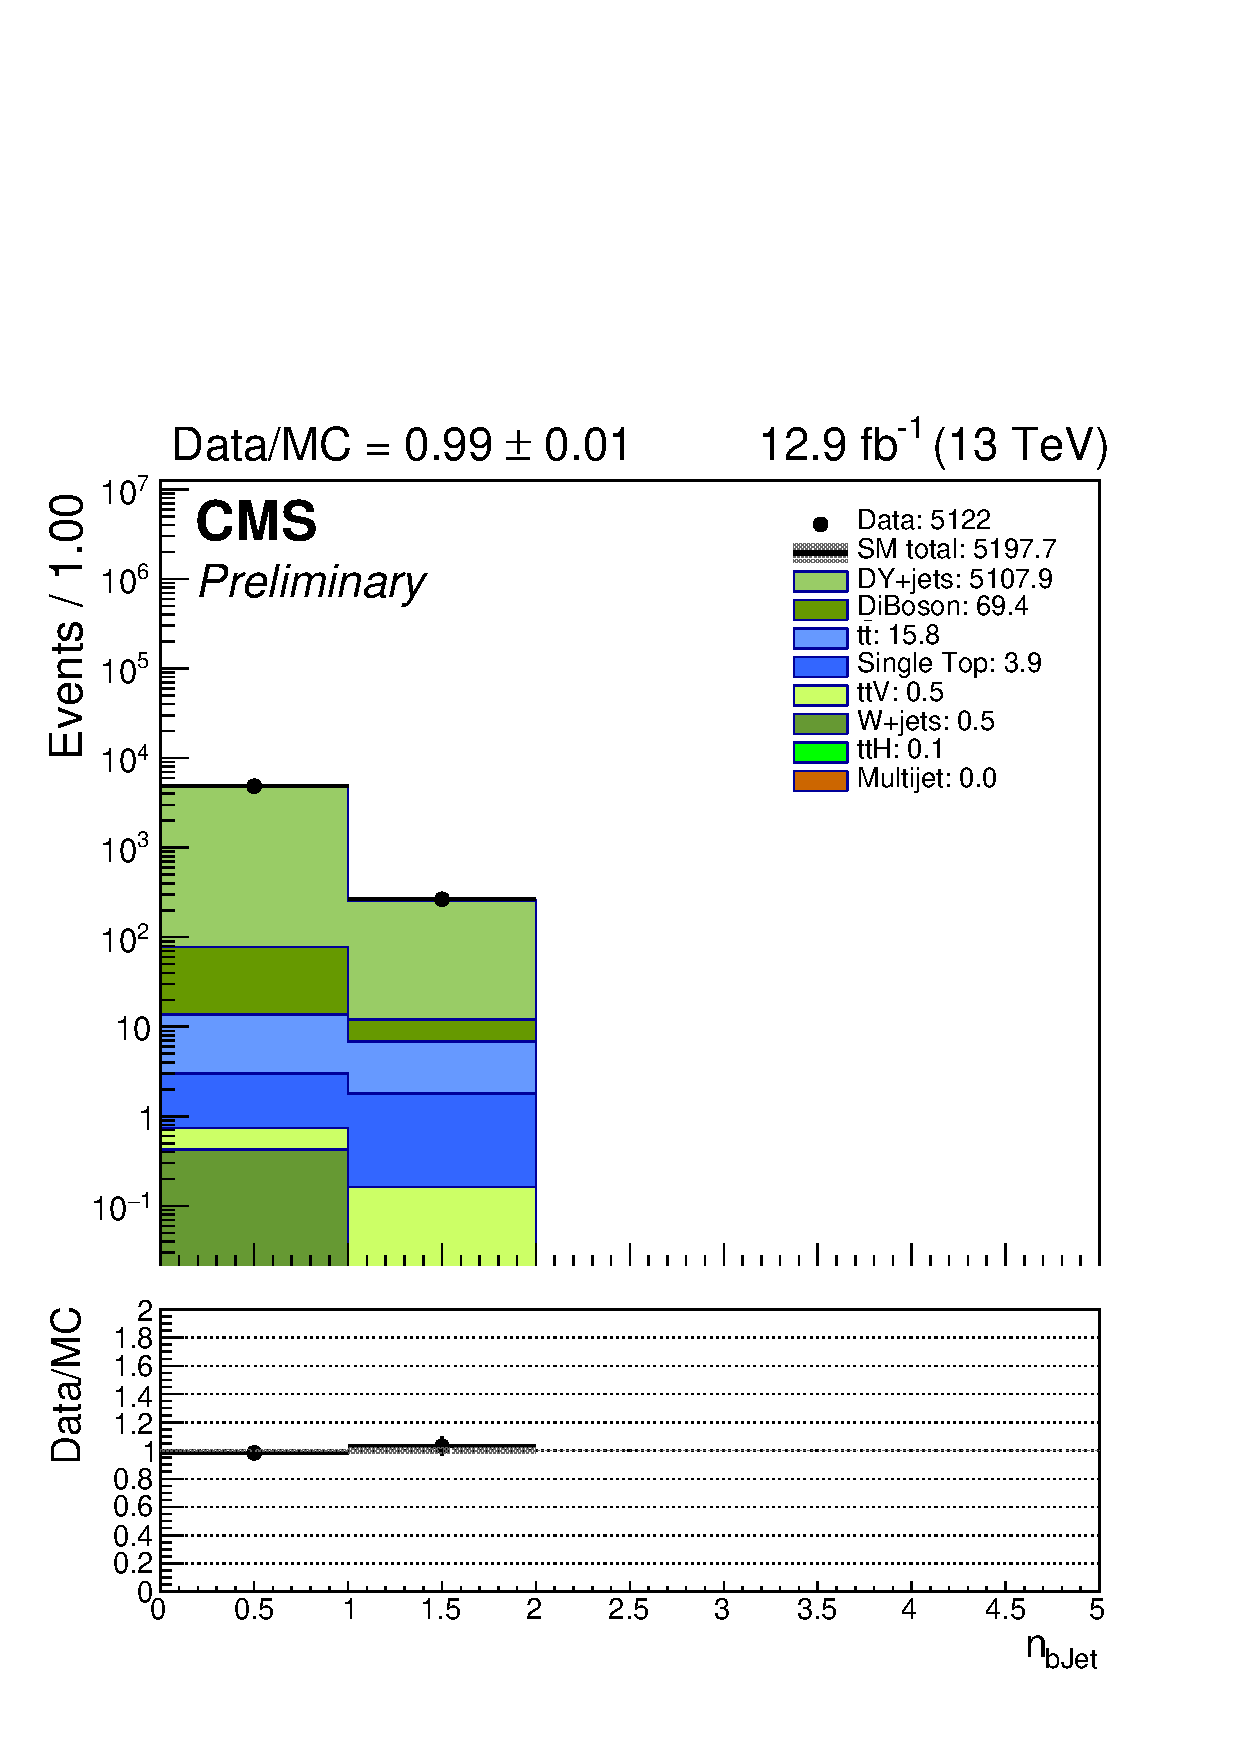
\includegraphics[width=0.5\textwidth]{figs/analysis/distributions/DoubleMu/nBJet40_eq1j.pdf}} ~~
        \subfloat {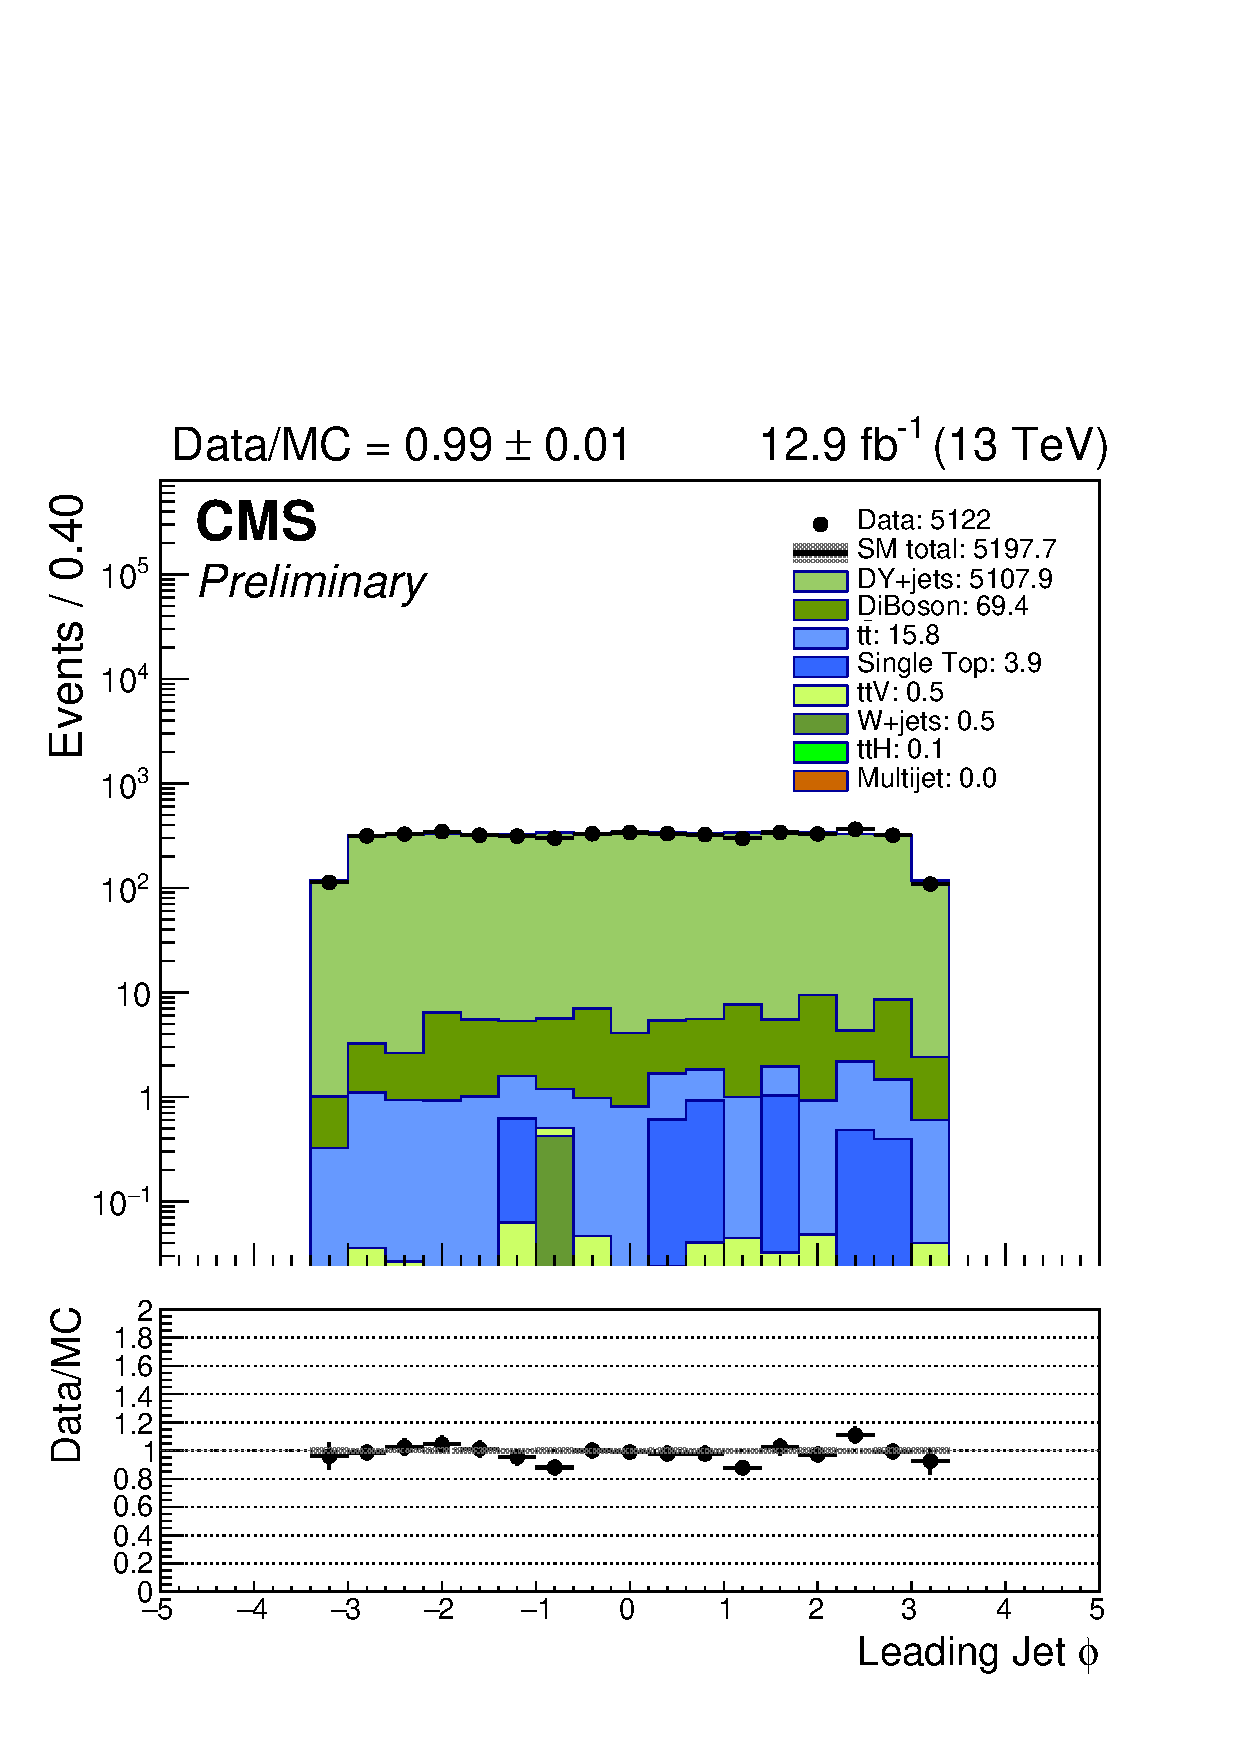
\includegraphics[width=0.5\textwidth]{figs/analysis/distributions/DoubleMu/jet_phi[0]_eq1j.pdf}} \\
        \caption{Key analysis variables for double muon control region (monojet bins)}
        \label{fig:distribution_doublemu_mono}
    \end{center}
\end{figure}

% \clearpage
% \subsection{Yields and distributions for the photon + jets control sample}

\begin{figure}
    \begin{center}
        \subfloat {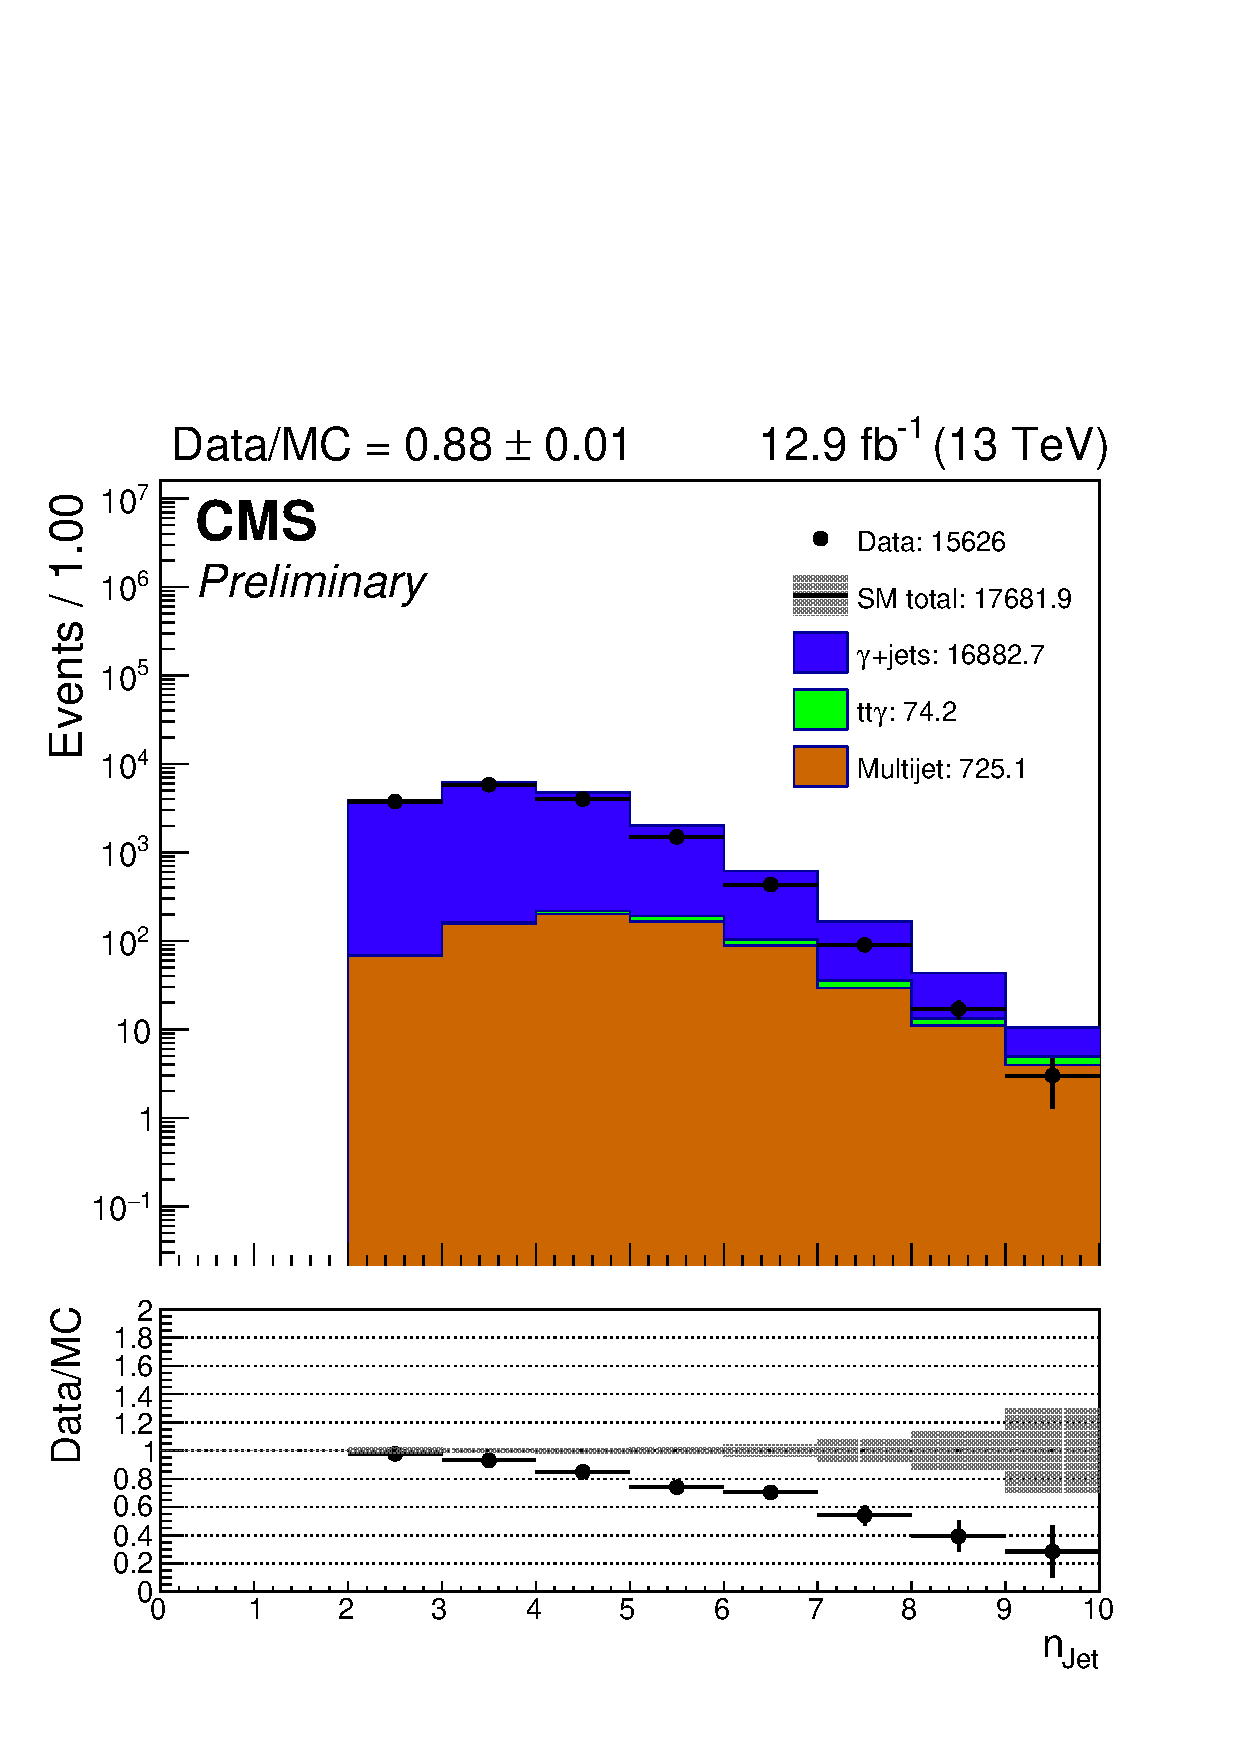
\includegraphics[width=0.5\textwidth]{figs/analysis/distributions/SinglePhoton/nJet40_sym.pdf}} ~~
        \subfloat {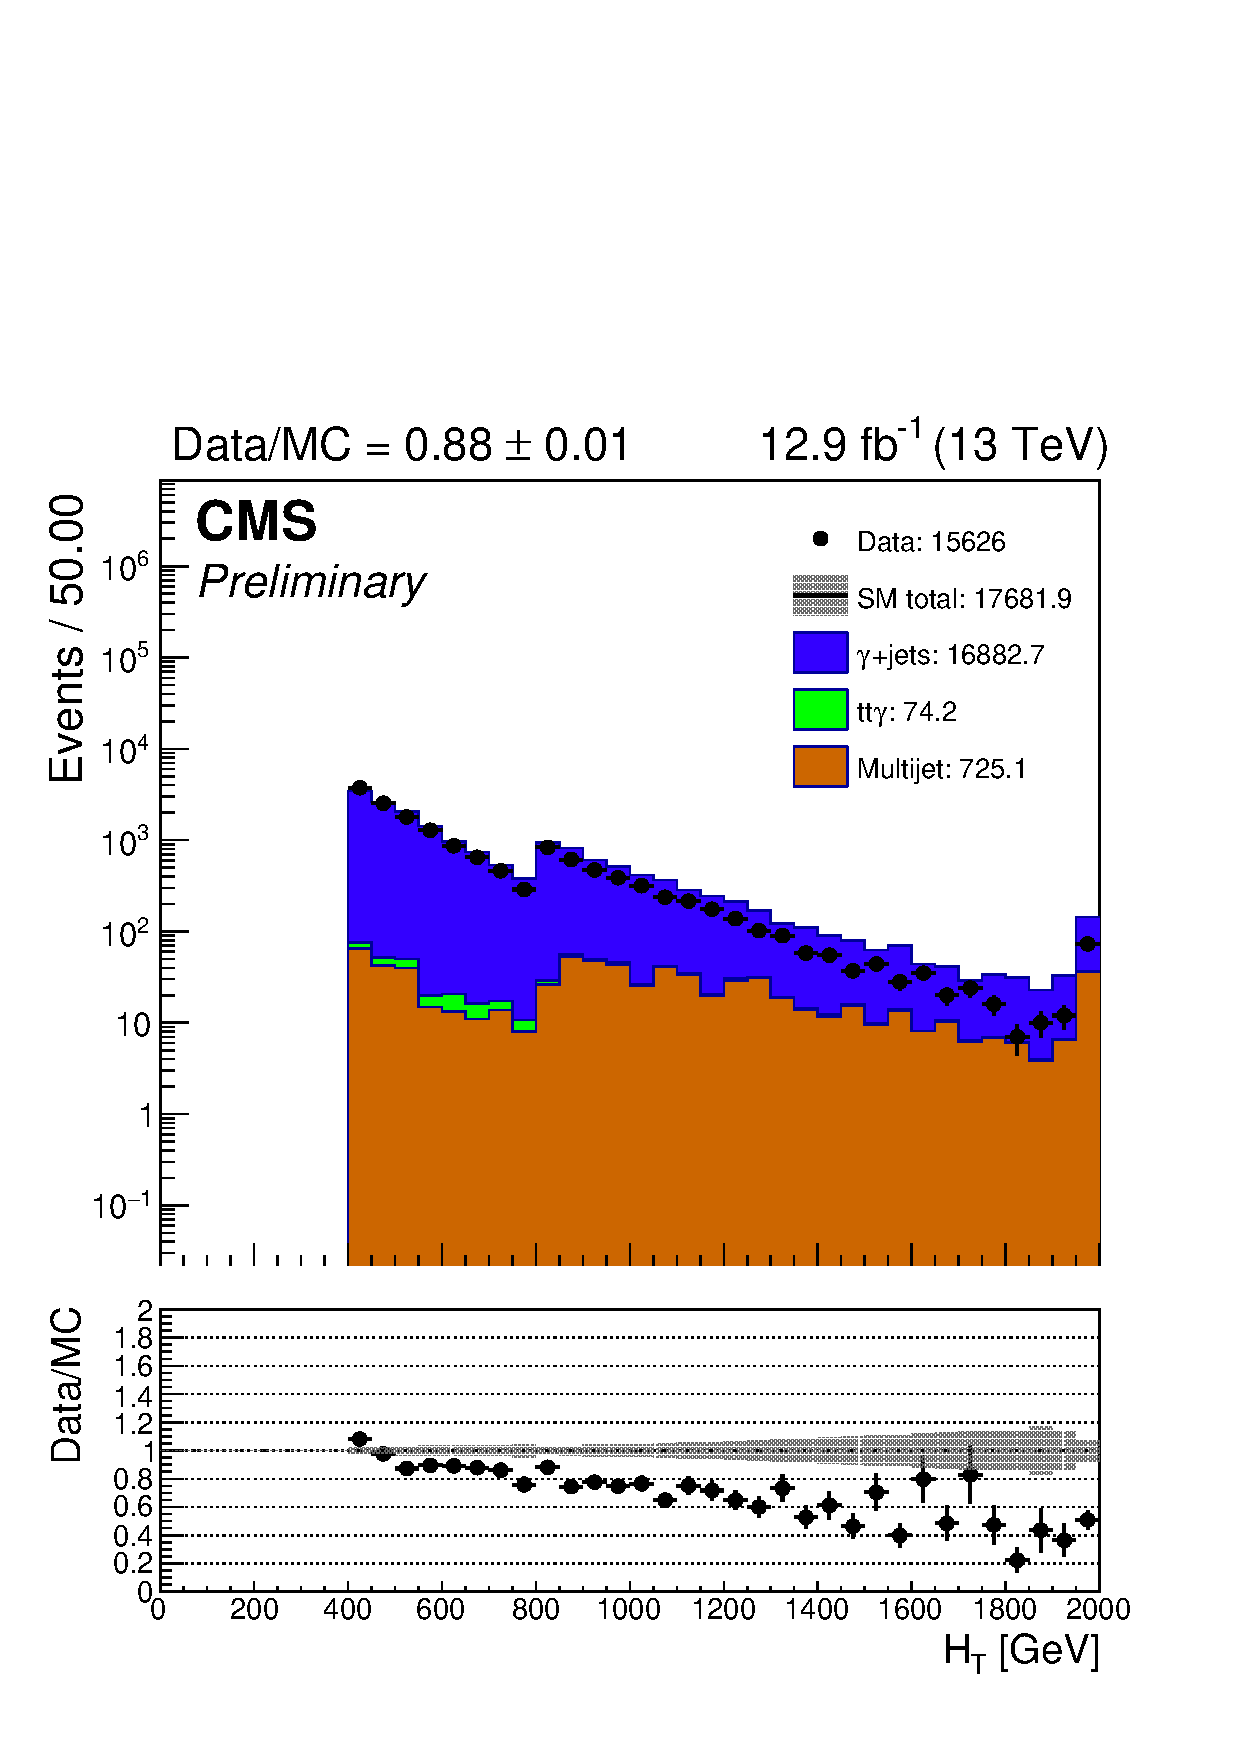
\includegraphics[width=0.5\textwidth]{figs/analysis/distributions/SinglePhoton/ht40_sym.pdf}} \\
        \subfloat {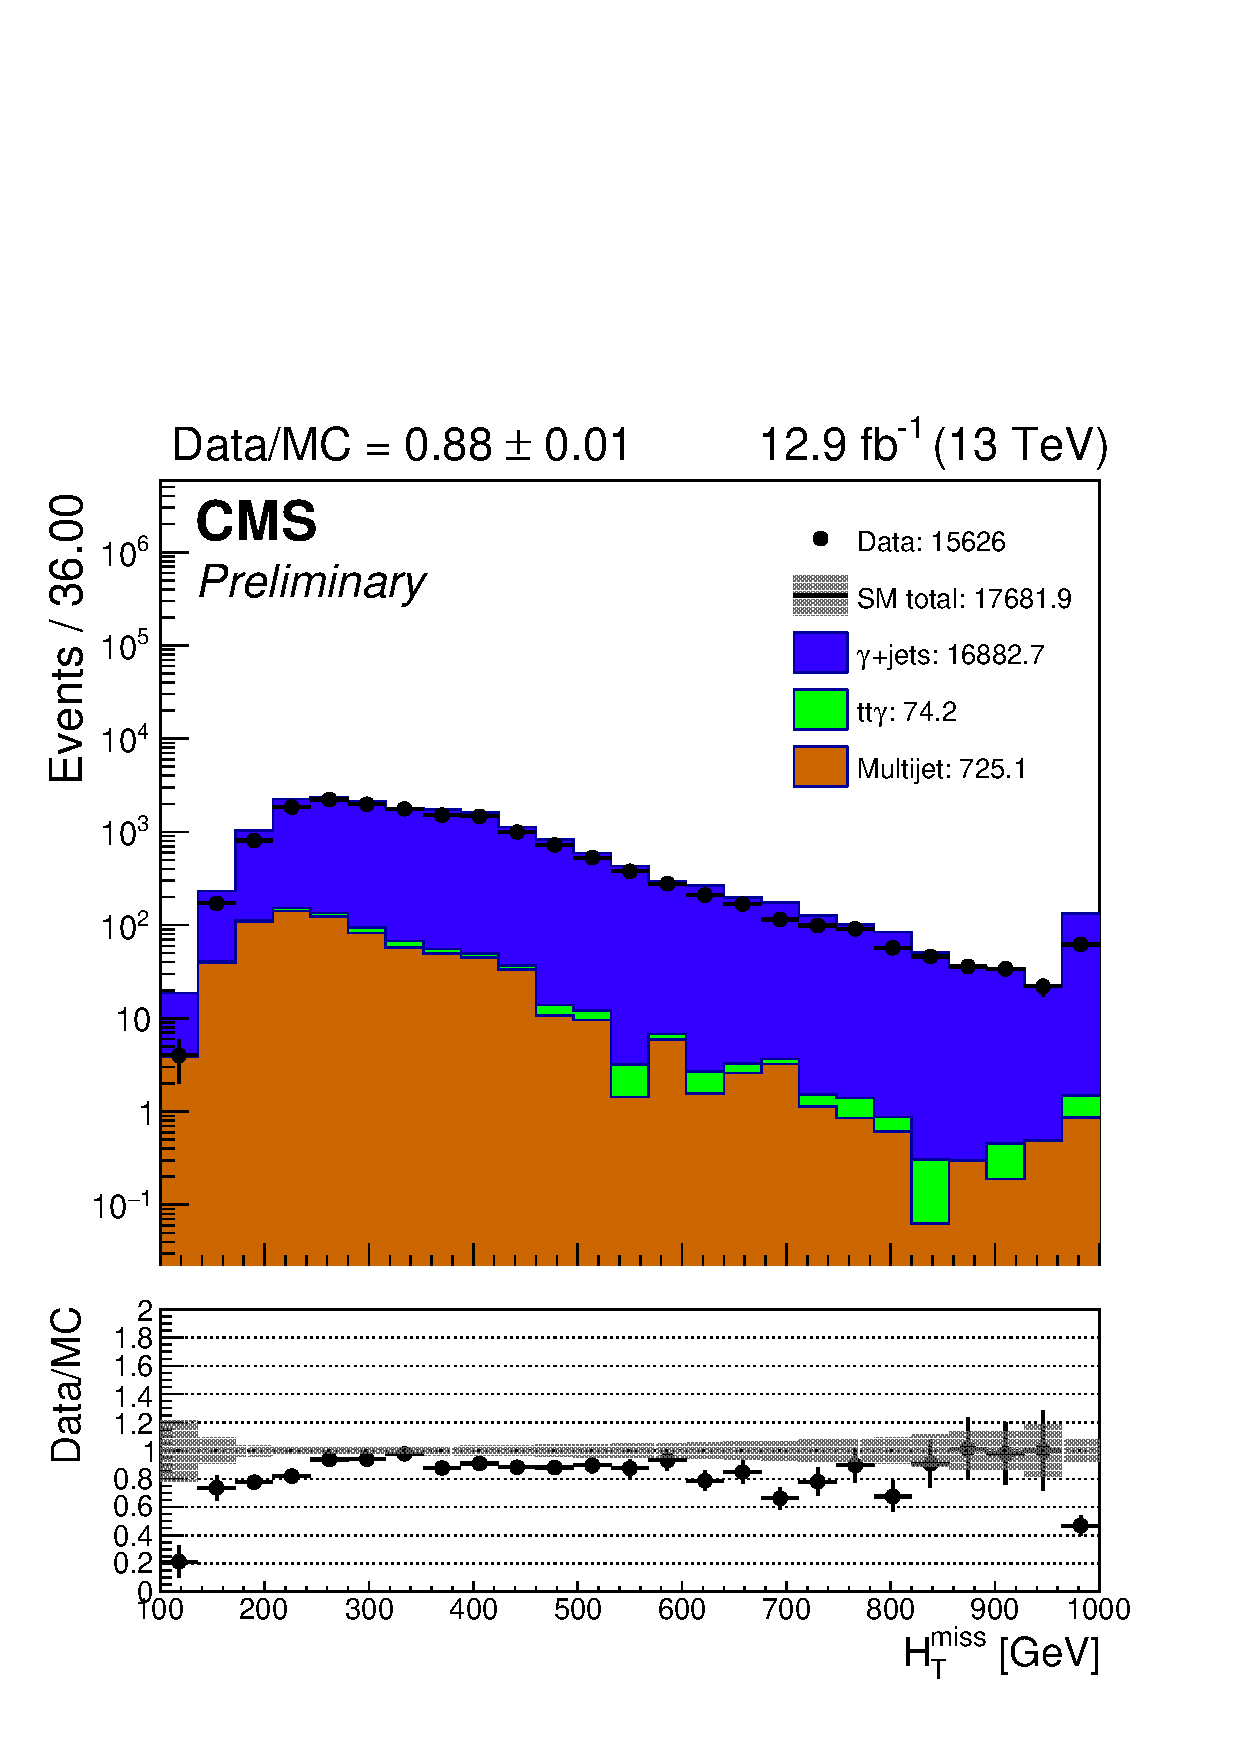
\includegraphics[width=0.5\textwidth]{figs/analysis/distributions/SinglePhoton/mht40_pt_sym.pdf}} ~~
        \subfloat {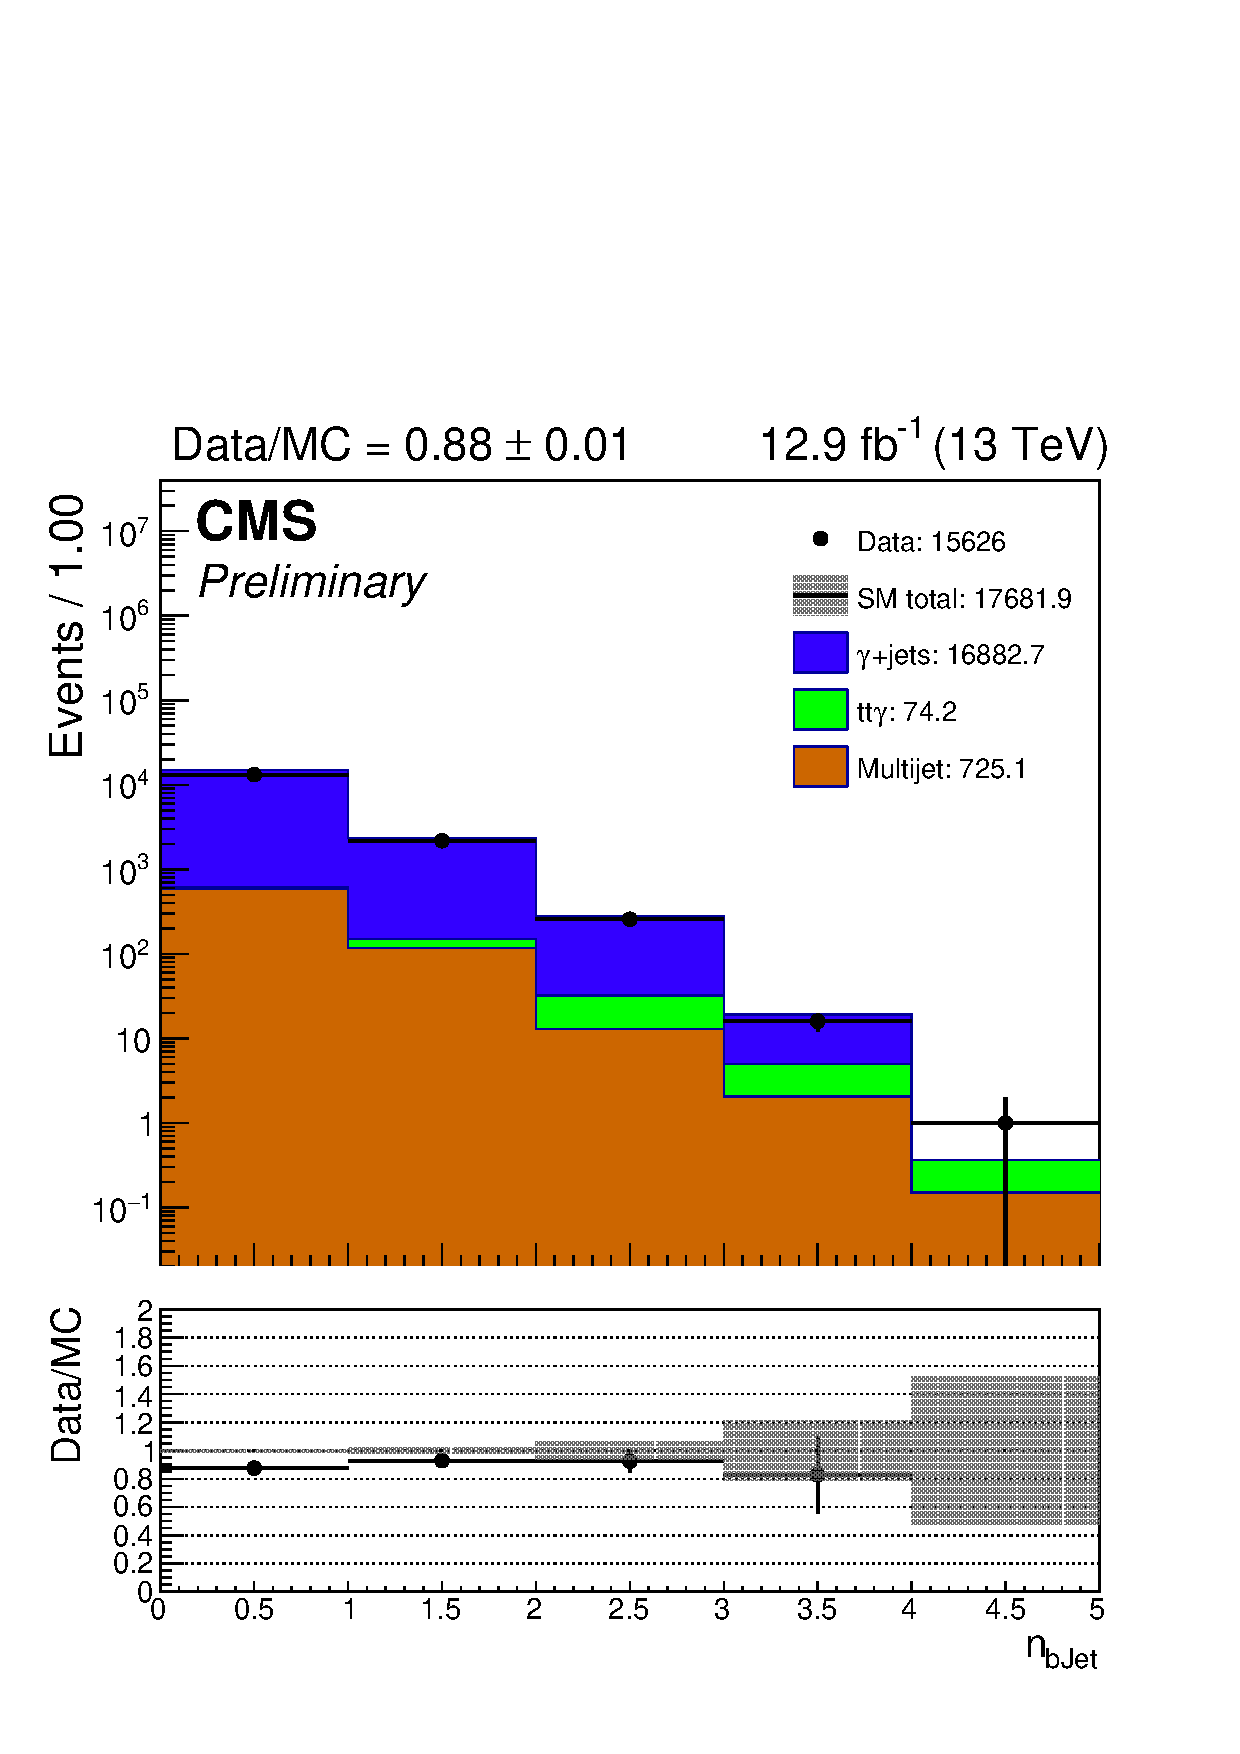
\includegraphics[width=0.5\textwidth]{figs/analysis/distributions/SinglePhoton/nBJet40_sym.pdf}} \\
        \caption{Key analysis variables for single photon control region (symmetric \njet bins)}
        \label{fig:distribution_singlephoton_sym}
    \end{center}
\end{figure}

\clearpage
\begin{figure}[h]
    \begin{center}
        \subfloat {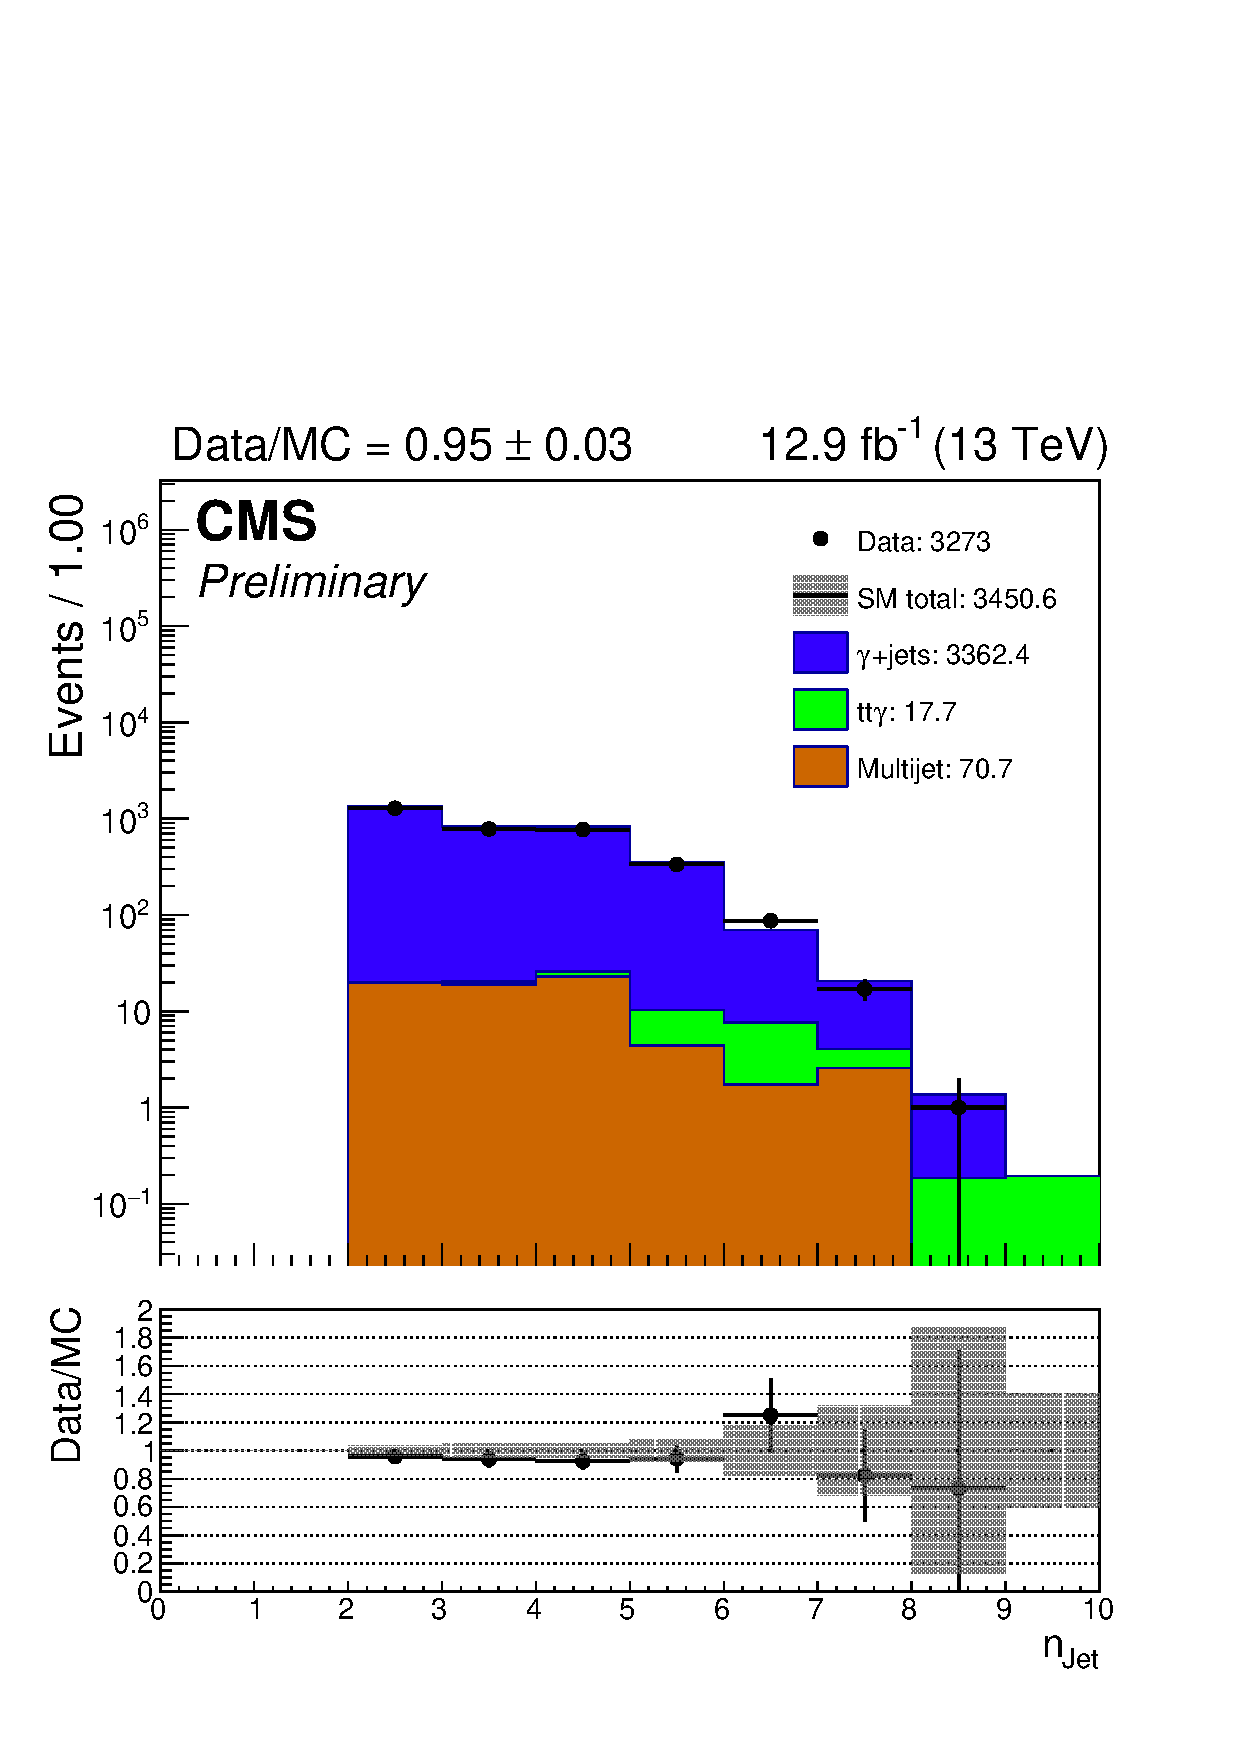
\includegraphics[width=0.5\textwidth]{figs/analysis/distributions/SinglePhoton/nJet40_asym.pdf}} ~~
        \subfloat {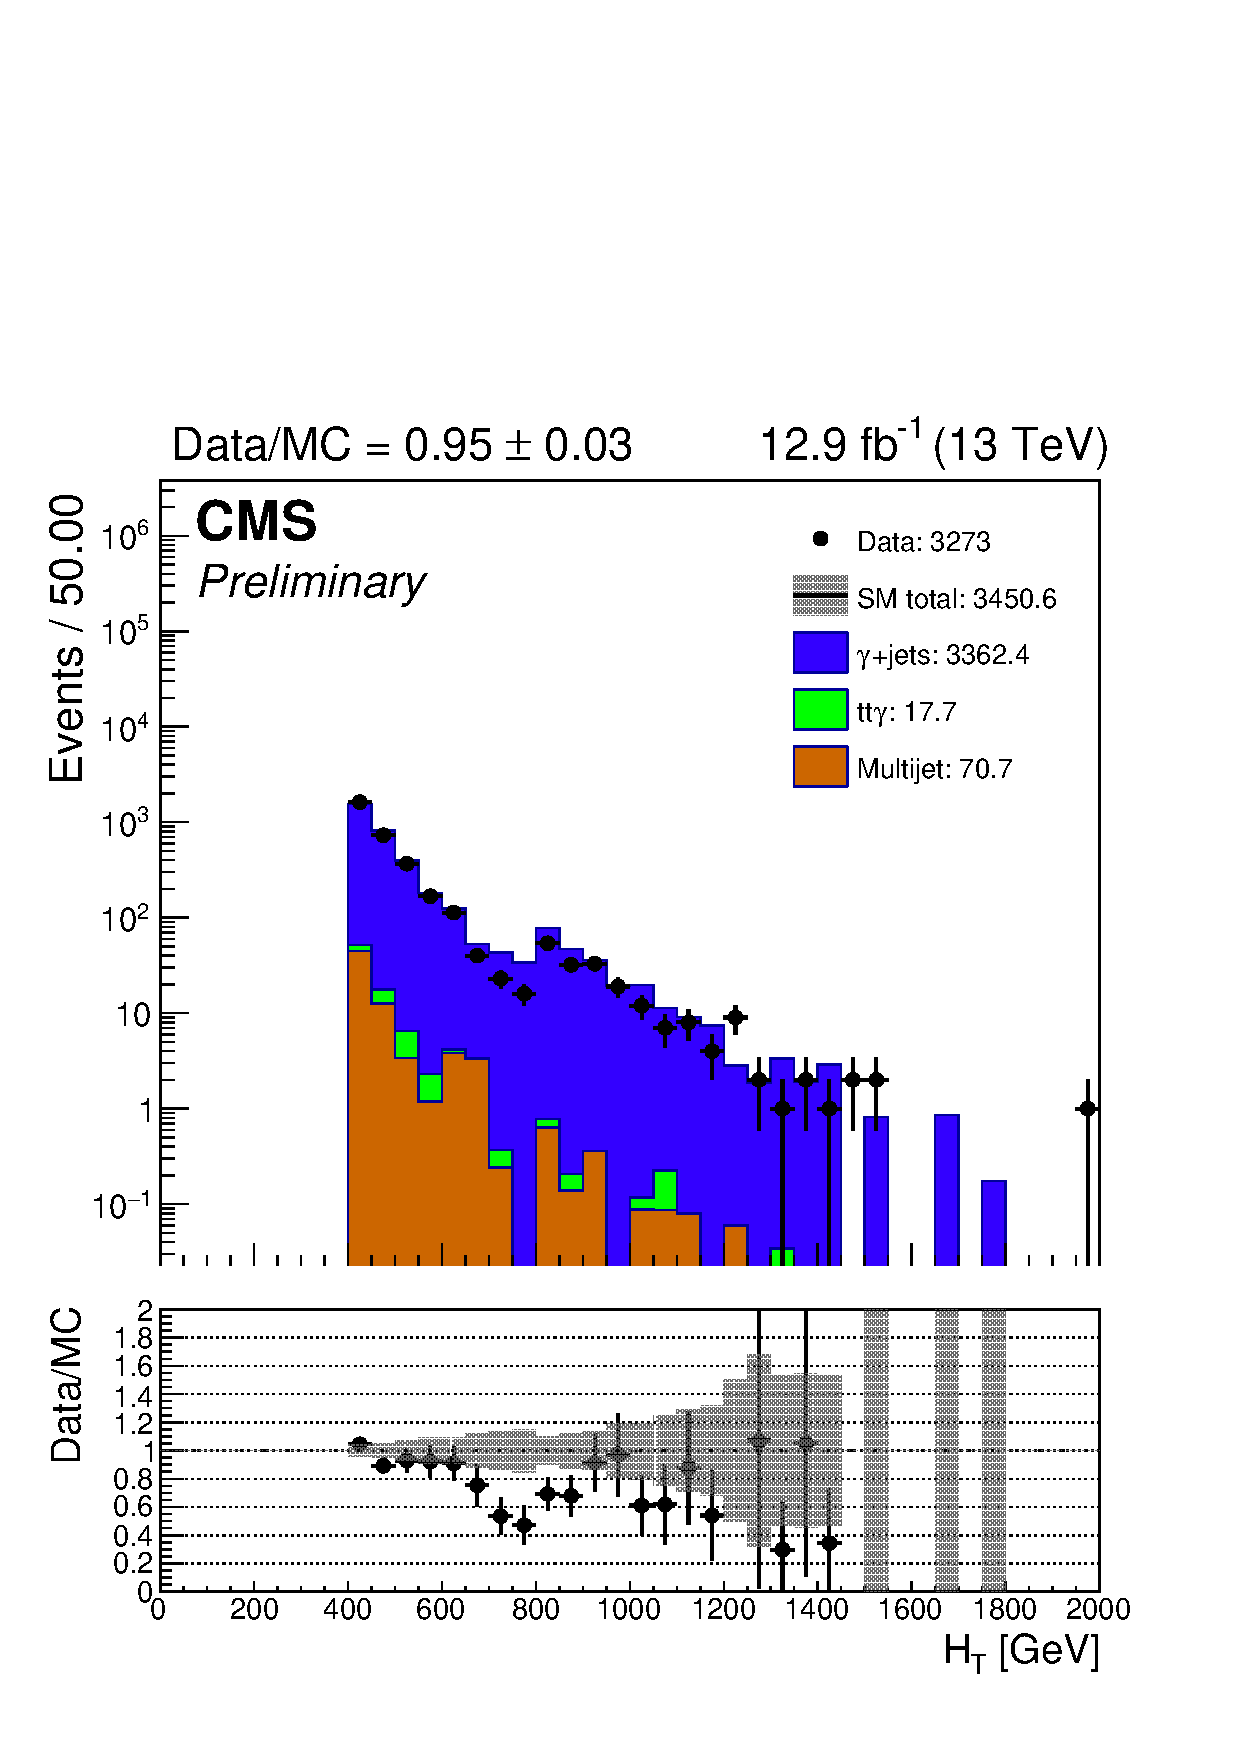
\includegraphics[width=0.5\textwidth]{figs/analysis/distributions/SinglePhoton/ht40_asym.pdf}} \\
        \subfloat {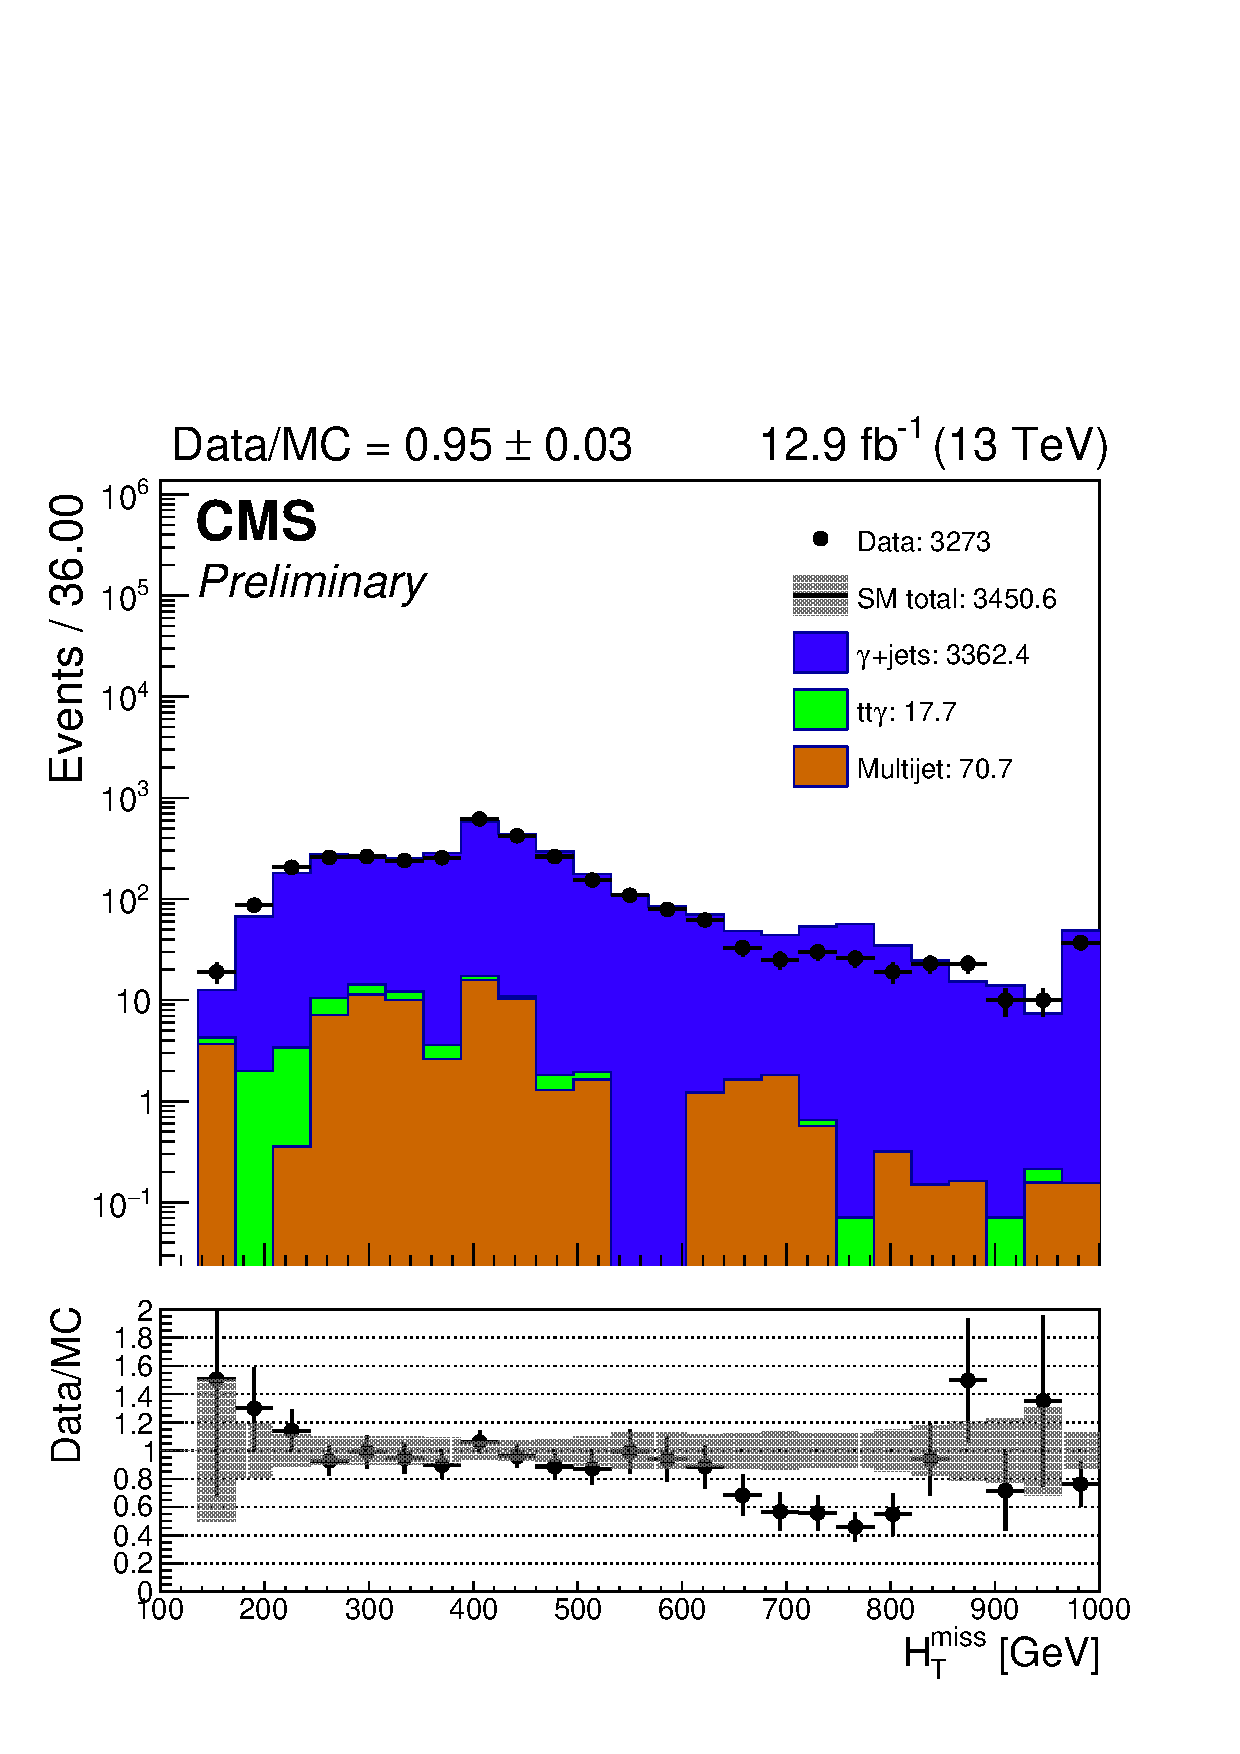
\includegraphics[width=0.5\textwidth]{figs/analysis/distributions/SinglePhoton/mht40_pt_asym.pdf}} ~~
        \subfloat {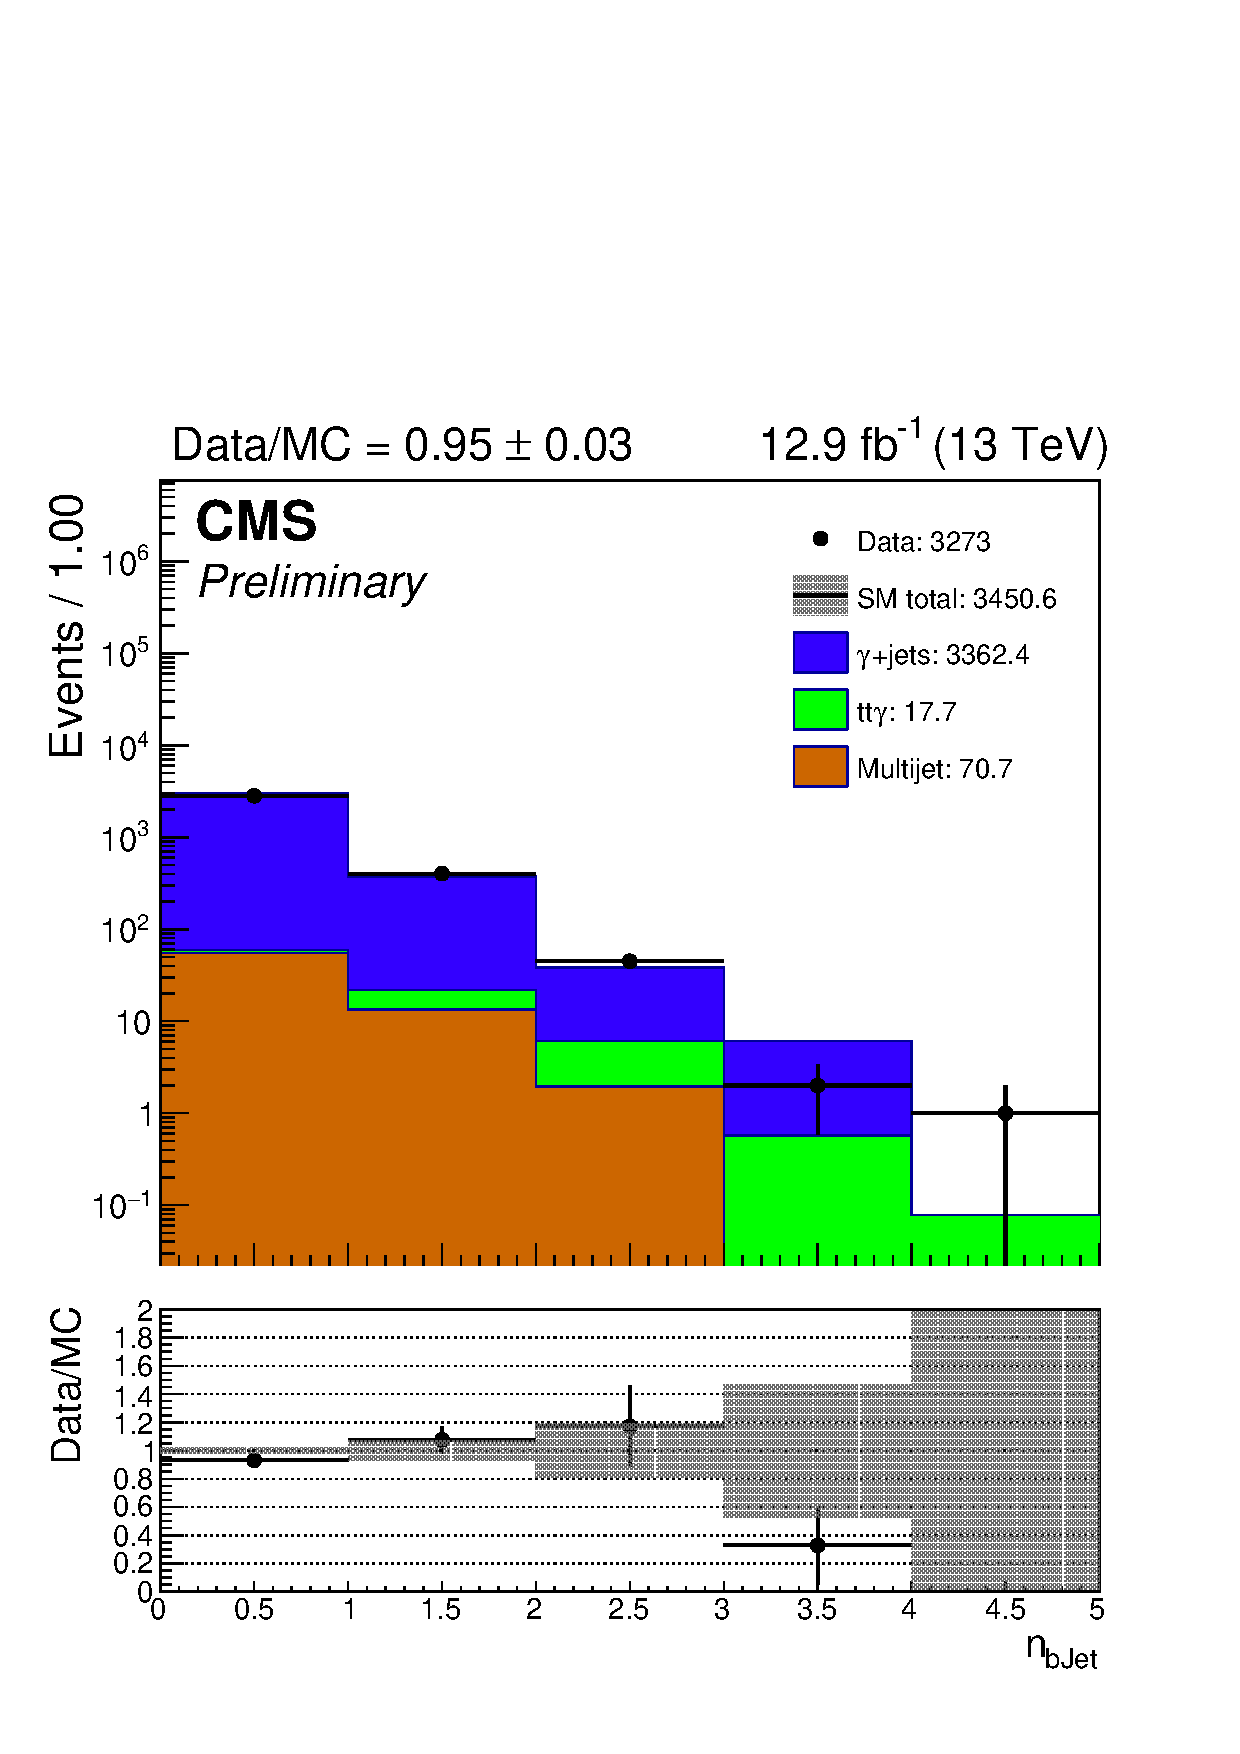
\includegraphics[width=0.5\textwidth]{figs/analysis/distributions/SinglePhoton/nBJet40_asym.pdf}} \\
        \caption{Key analysis variables for single photon control region (asymmetric \njet bins)}
        \label{fig:distribution_singlephoton_asym}
    \end{center}
\end{figure}

\clearpage
\begin{figure}
    \begin{center} 
        \subfloat {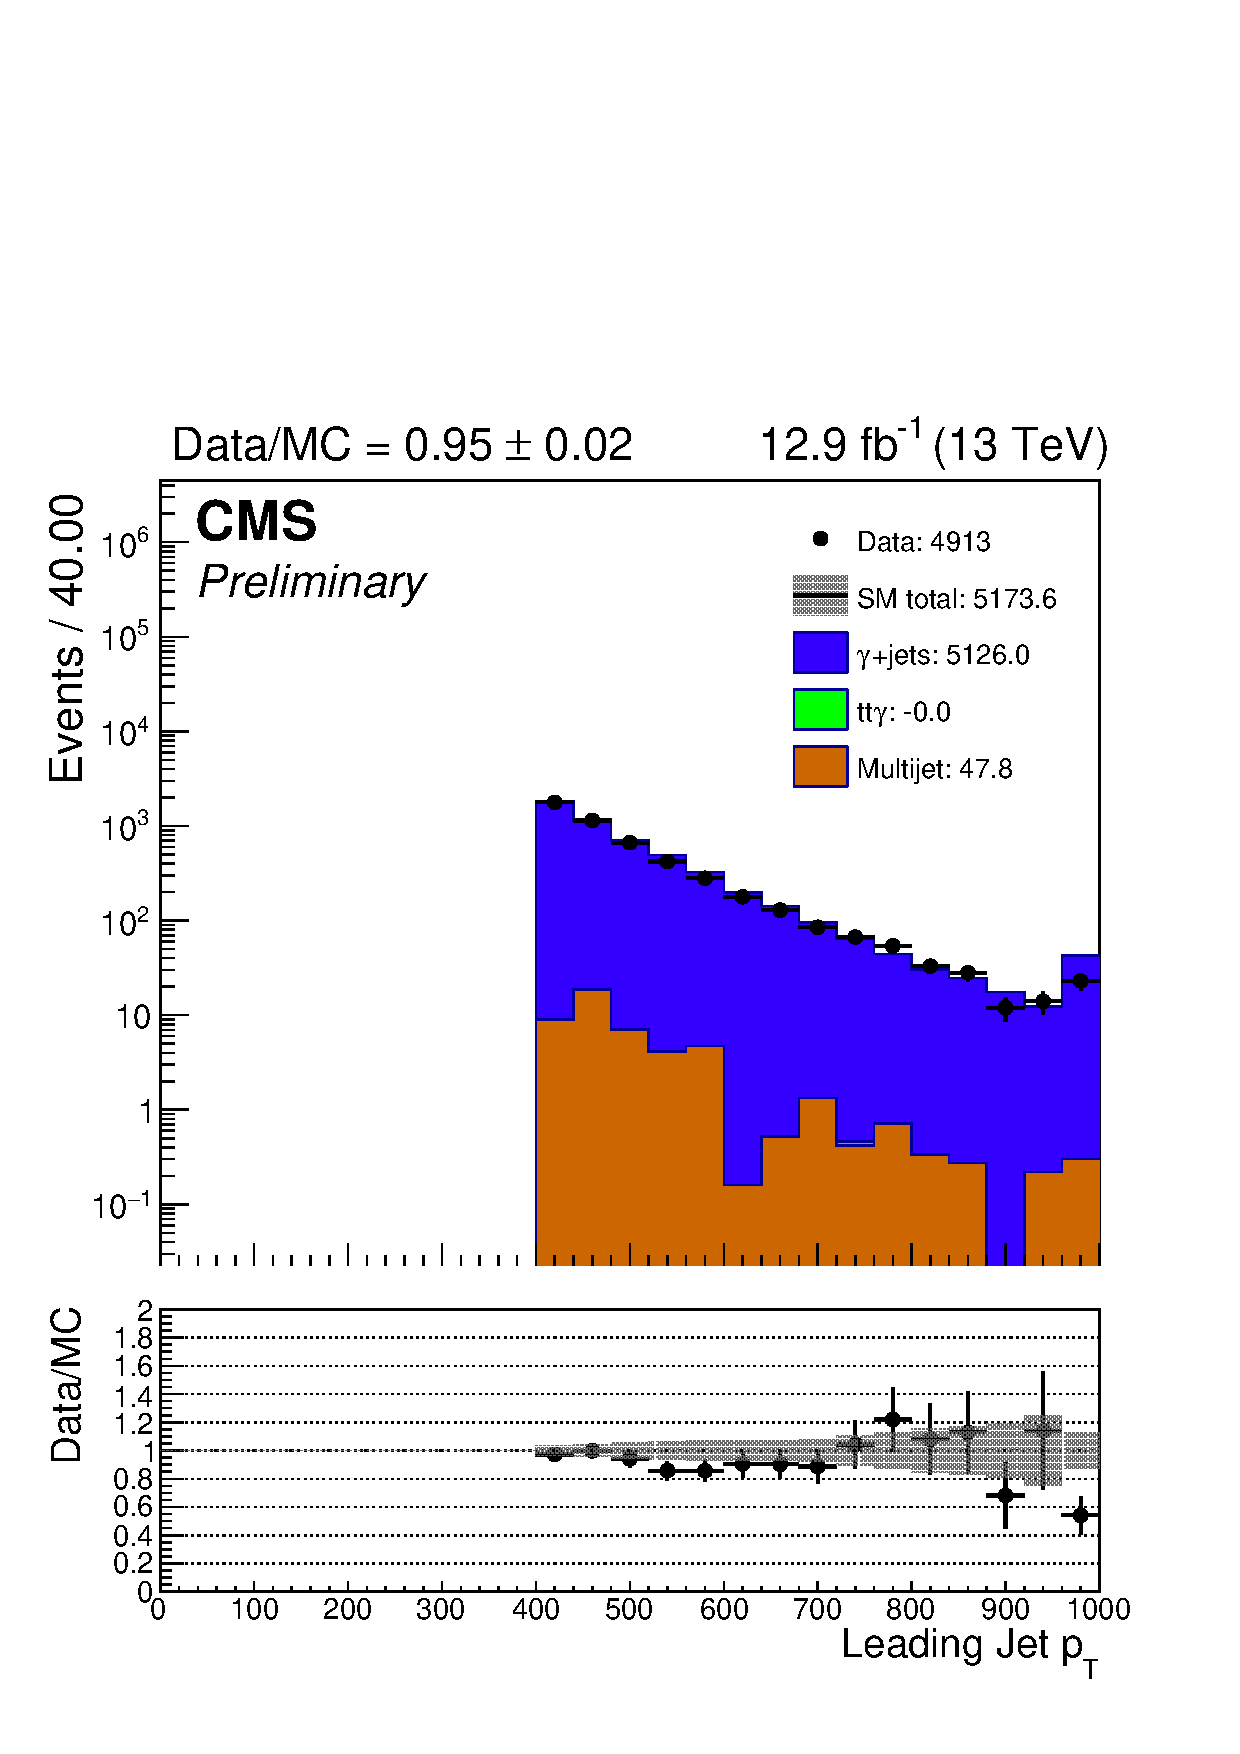
\includegraphics[width=0.5\textwidth]{figs/analysis/distributions/SinglePhoton/jet_pt[0]_eq1j.pdf}} ~~
        \subfloat {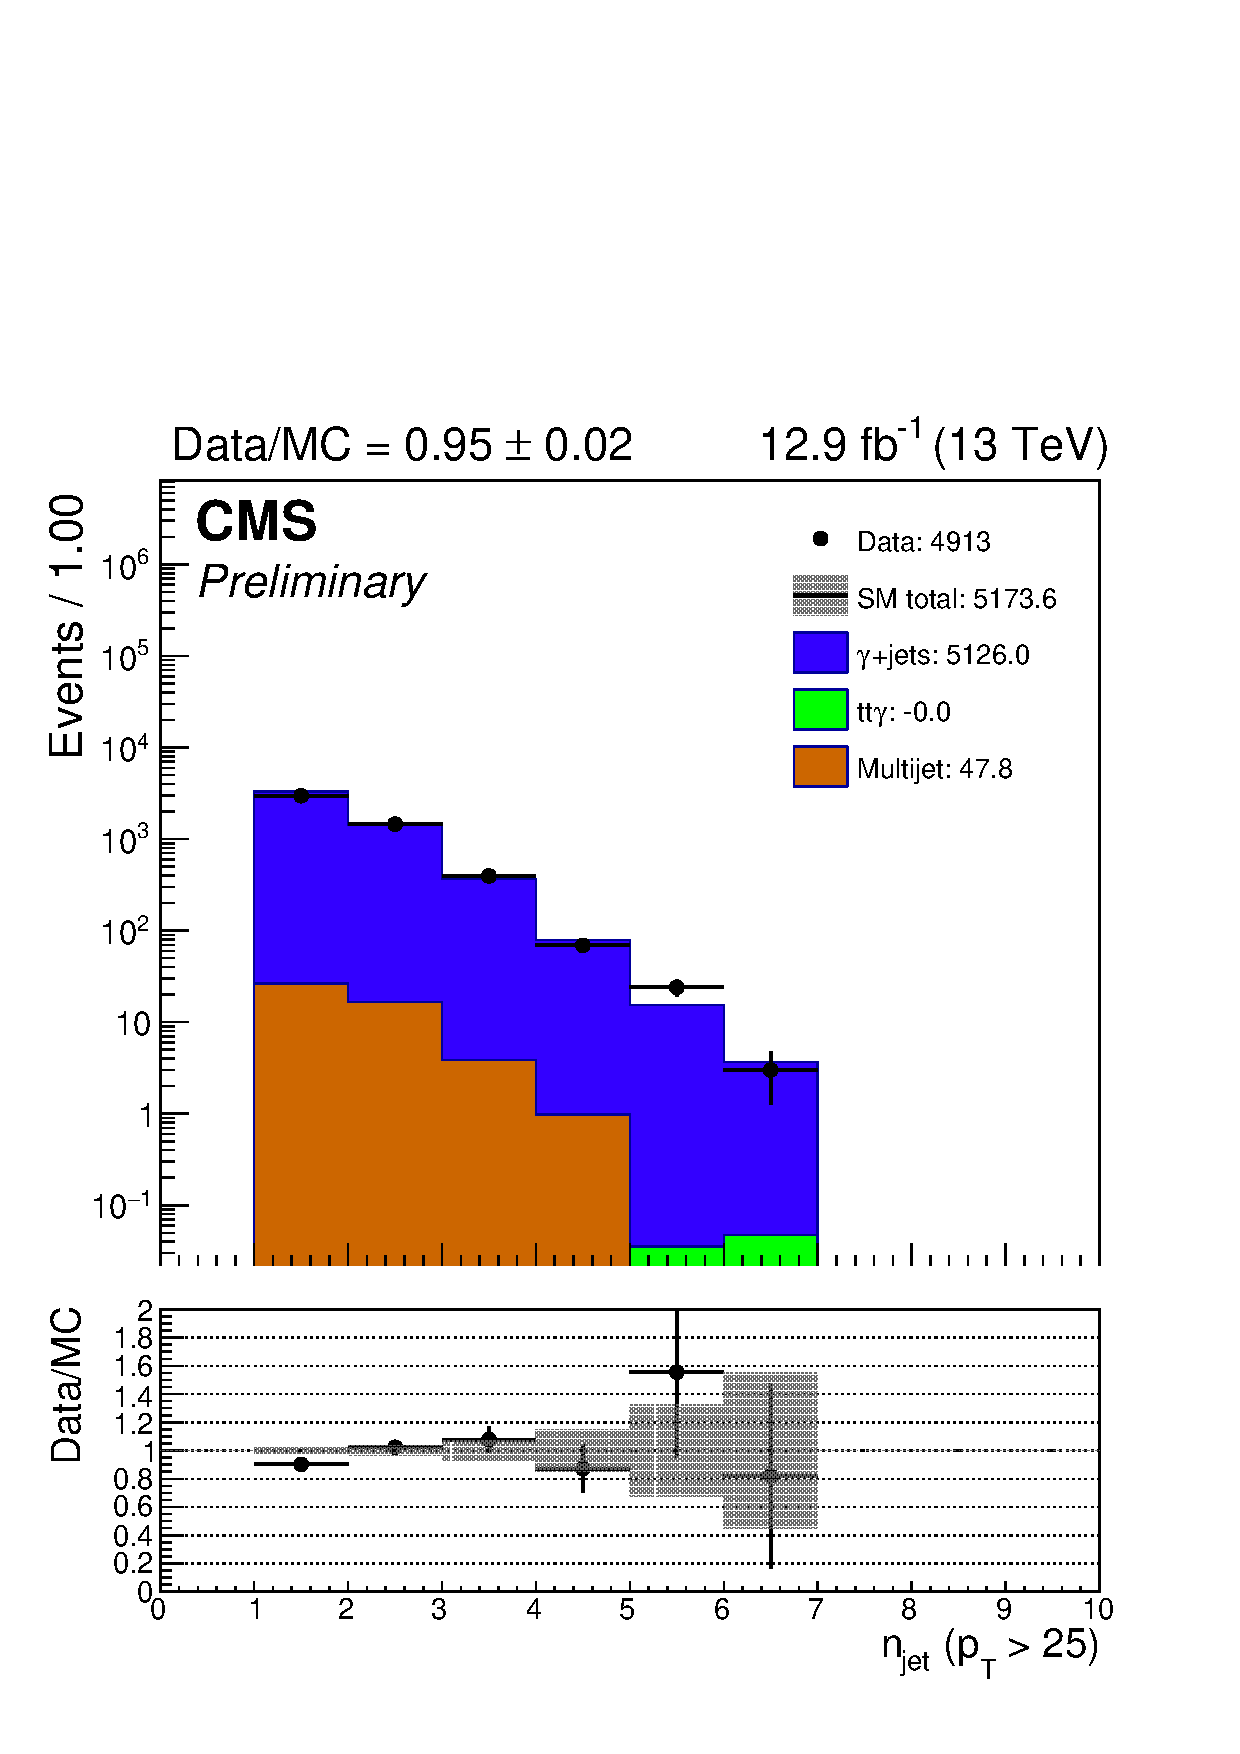
\includegraphics[width=0.5\textwidth]{figs/analysis/distributions/SinglePhoton/njetInc_eq1j.pdf}} \\
        \subfloat {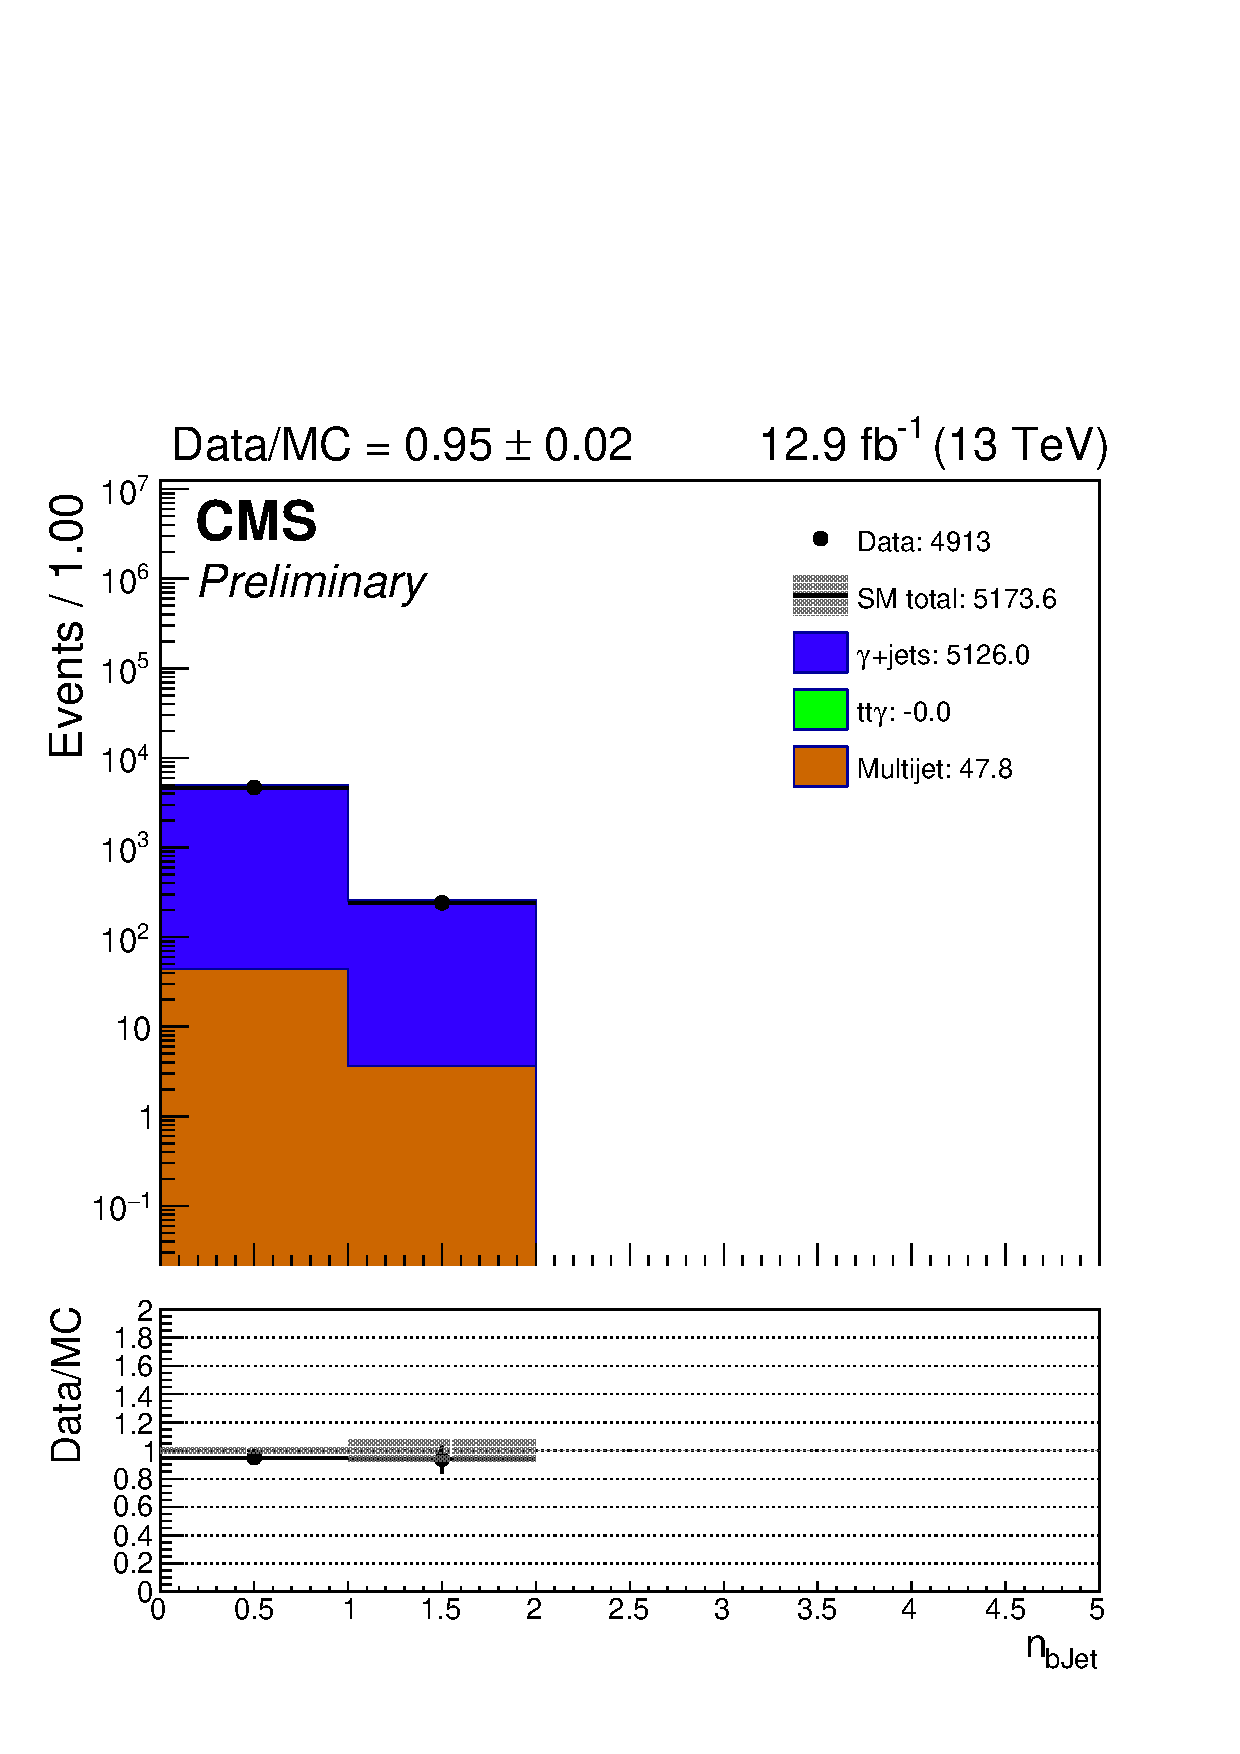
\includegraphics[width=0.5\textwidth]{figs/analysis/distributions/SinglePhoton/nBJet40_eq1j.pdf}} ~~
        \subfloat {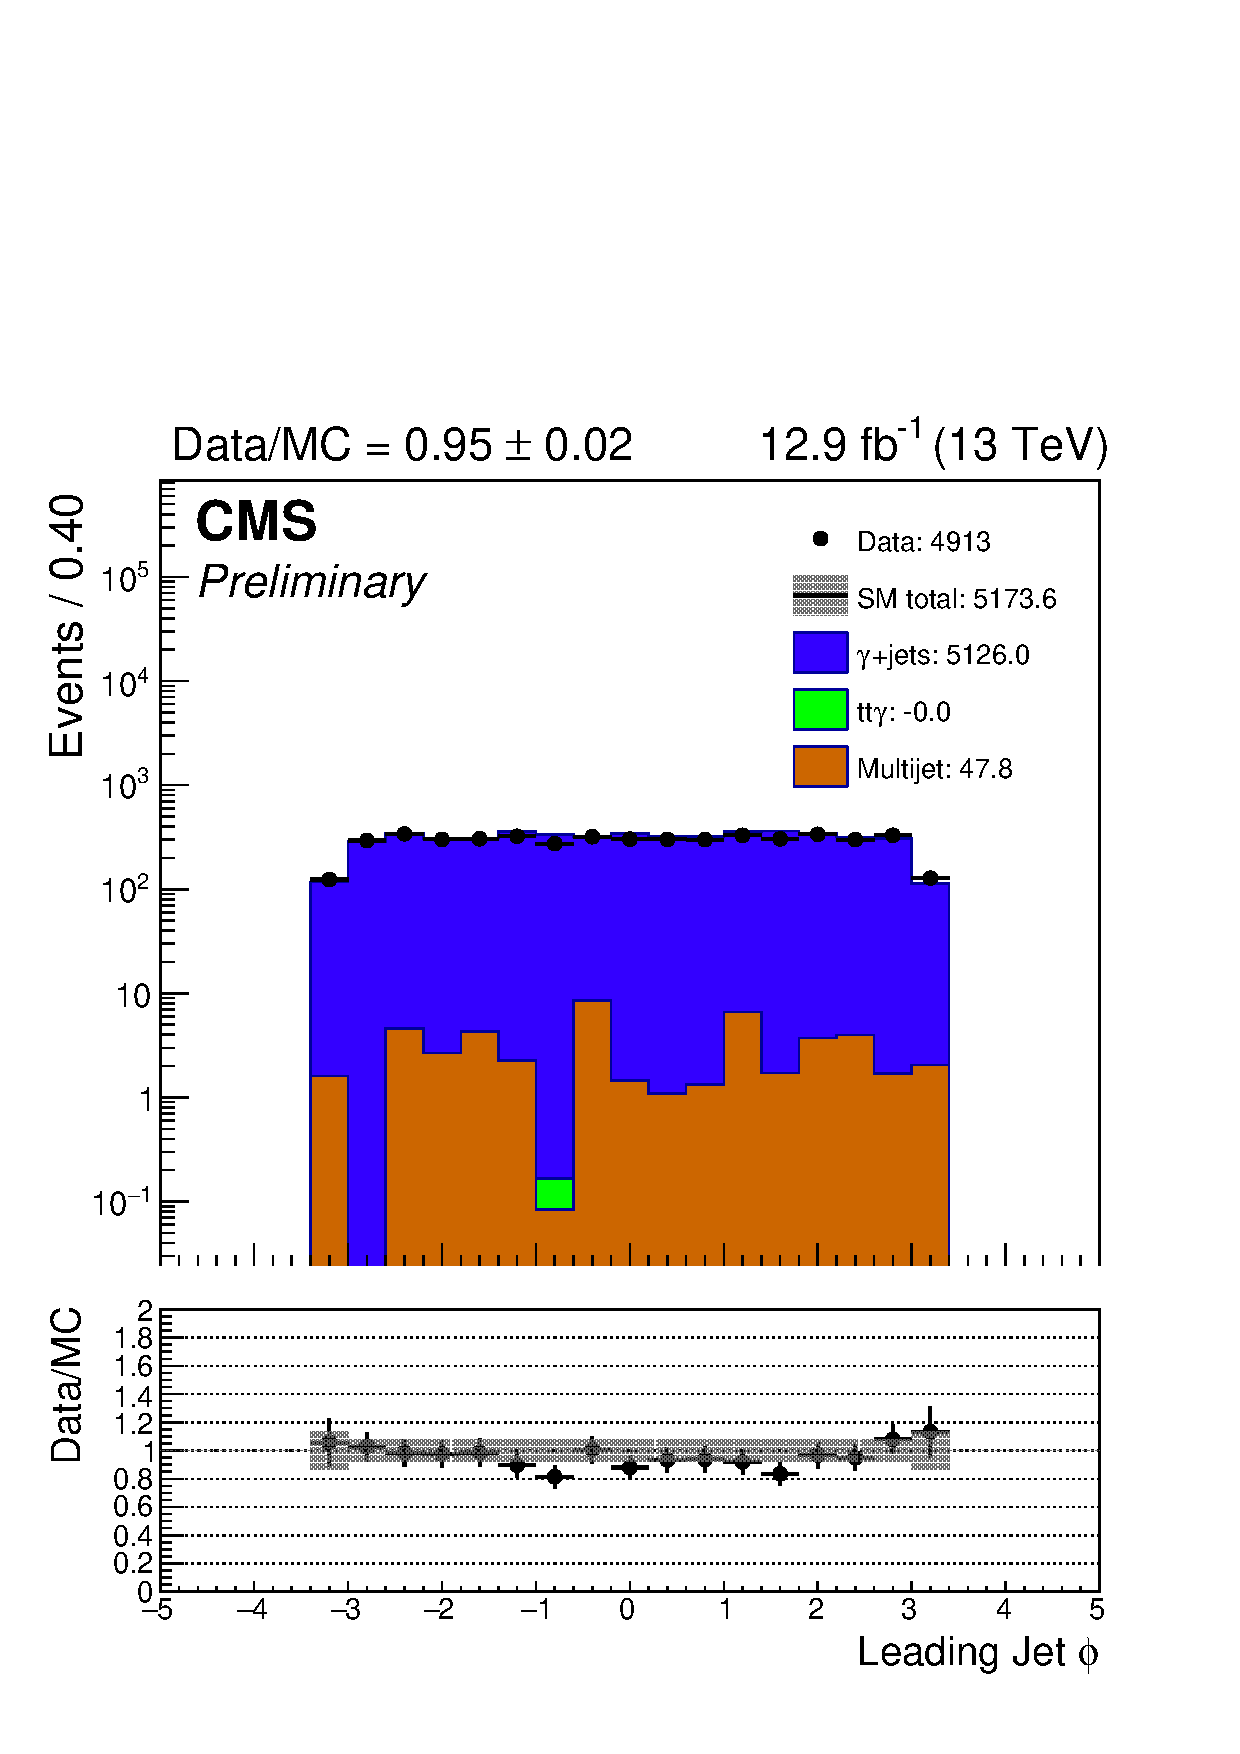
\includegraphics[width=0.5\textwidth]{figs/analysis/distributions/SinglePhoton/jet_phi[0]_eq1j.pdf}} \\
        \caption{Key analysis variables for single photon control region (monojet bins)}
        \label{fig:distribution_singlephoton_mono}
    \end{center}
\end{figure}

% \clearpage
% \subsection{Expected yields and distributions in the signal region}
\clearpage
\begin{figure}
    \begin{center}
        \subfloat {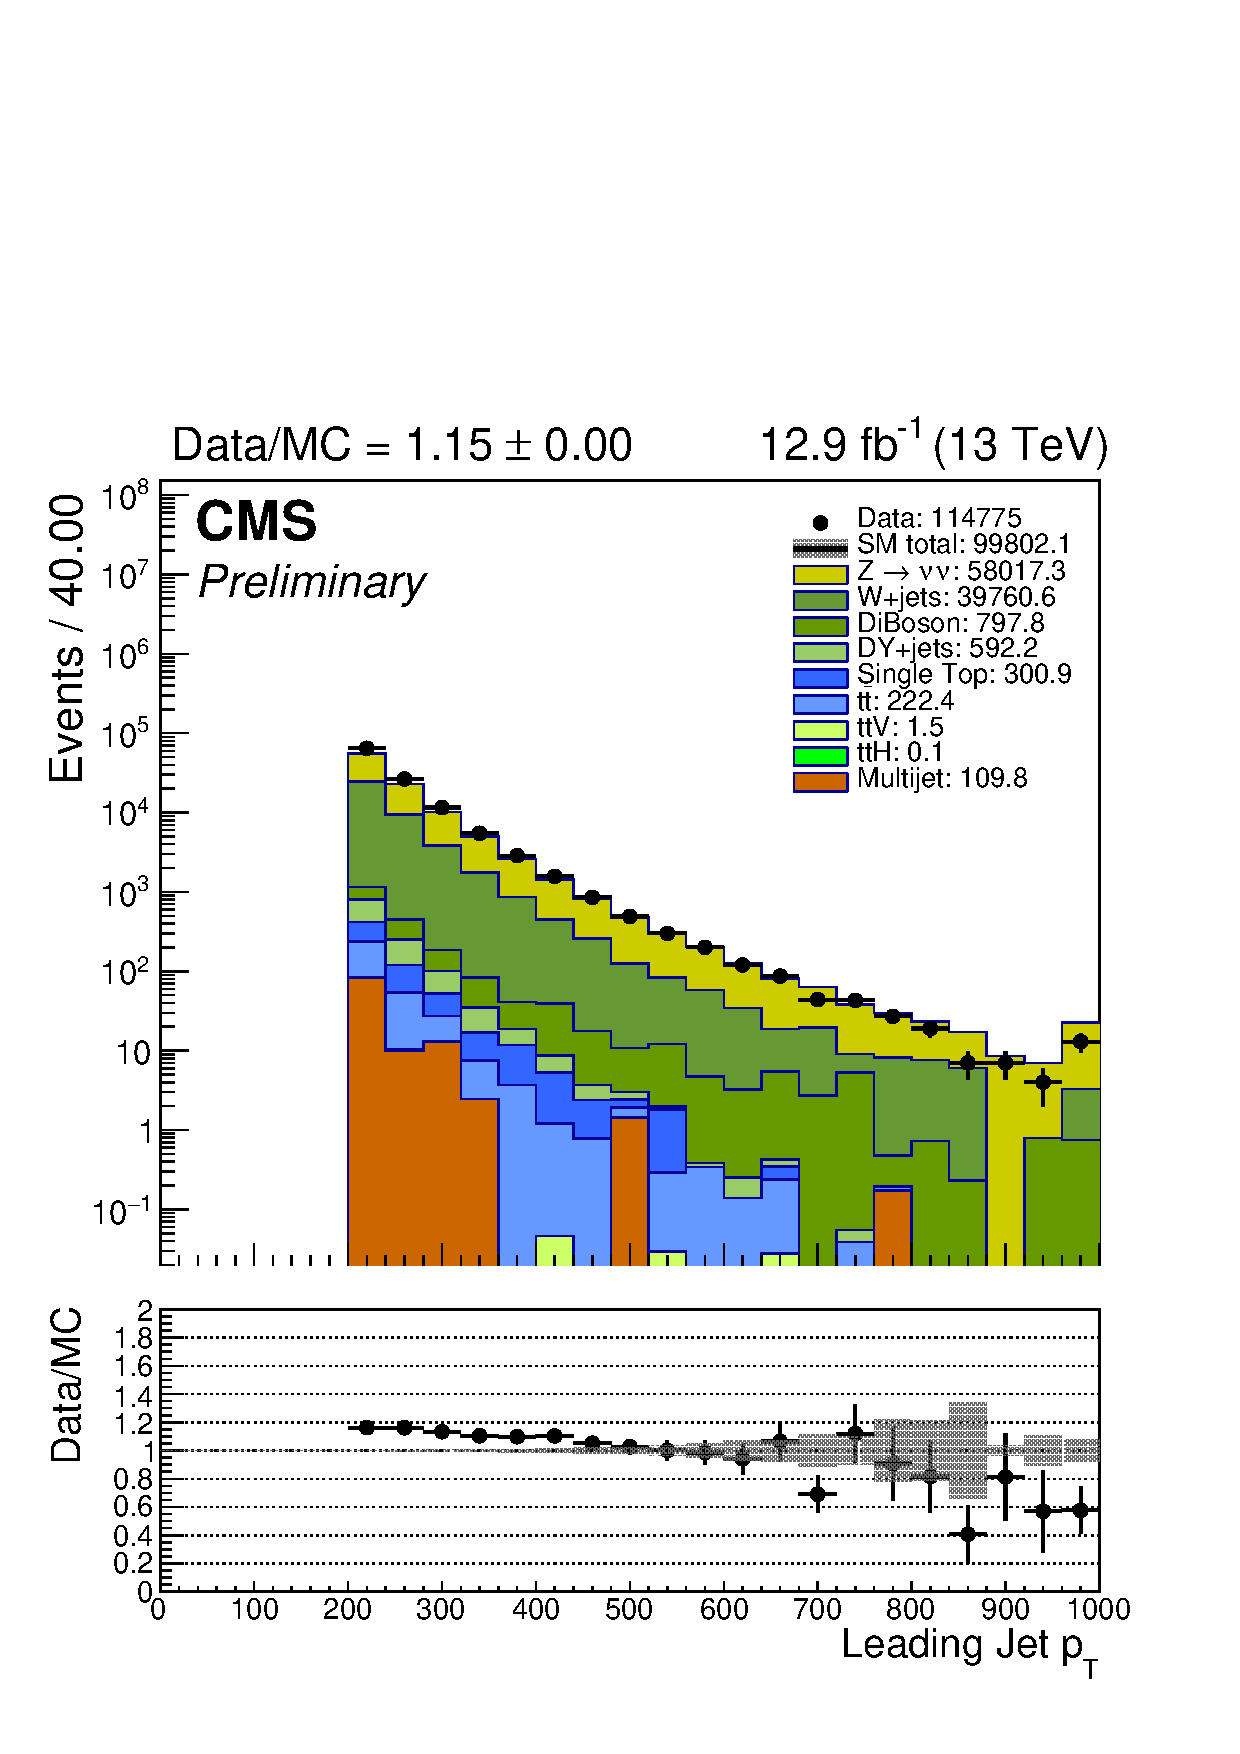
\includegraphics[width=0.5\textwidth]{figs/analysis/distributions/Signal/jet_pt[0]_eq1j.pdf}} ~~
        \subfloat {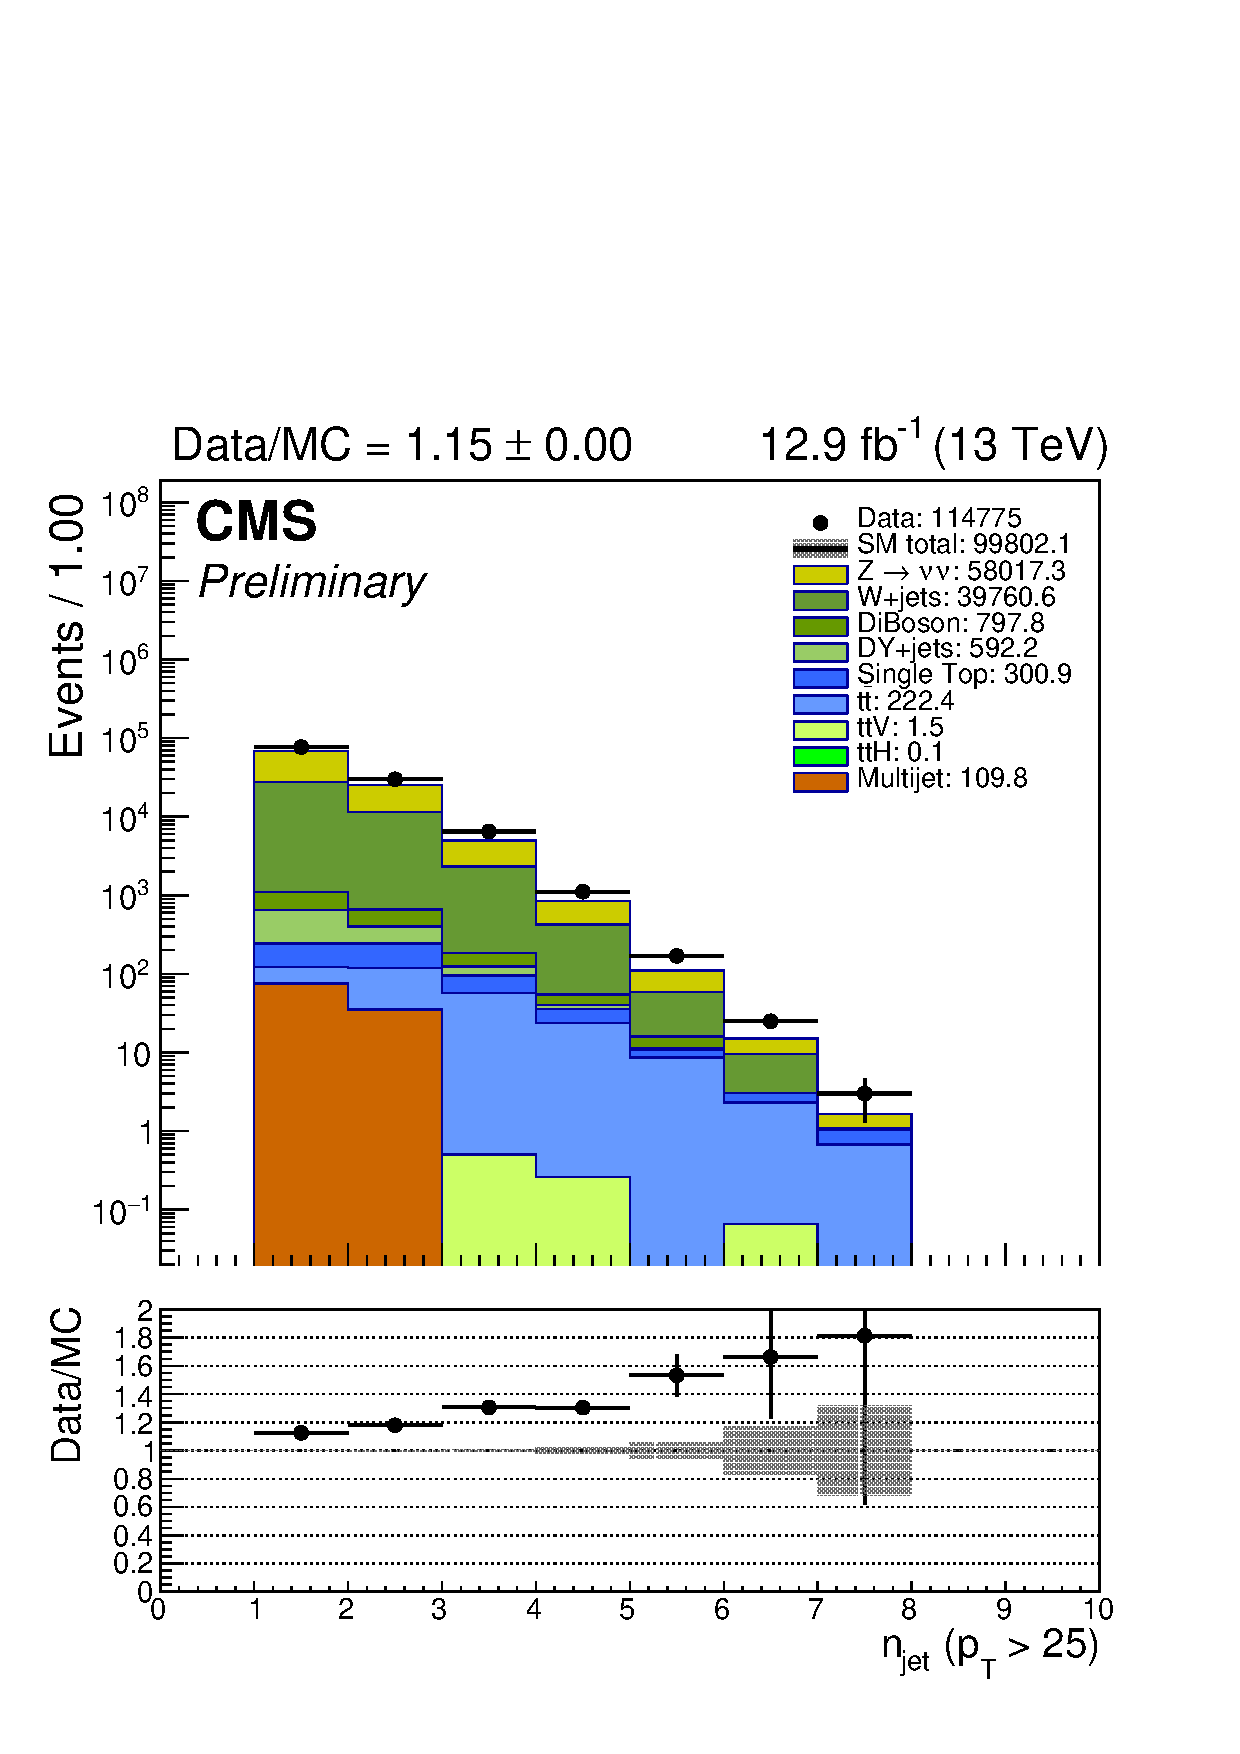
\includegraphics[width=0.5\textwidth]{figs/analysis/distributions/Signal/njetInc_eq1j.pdf}} \\
        \subfloat {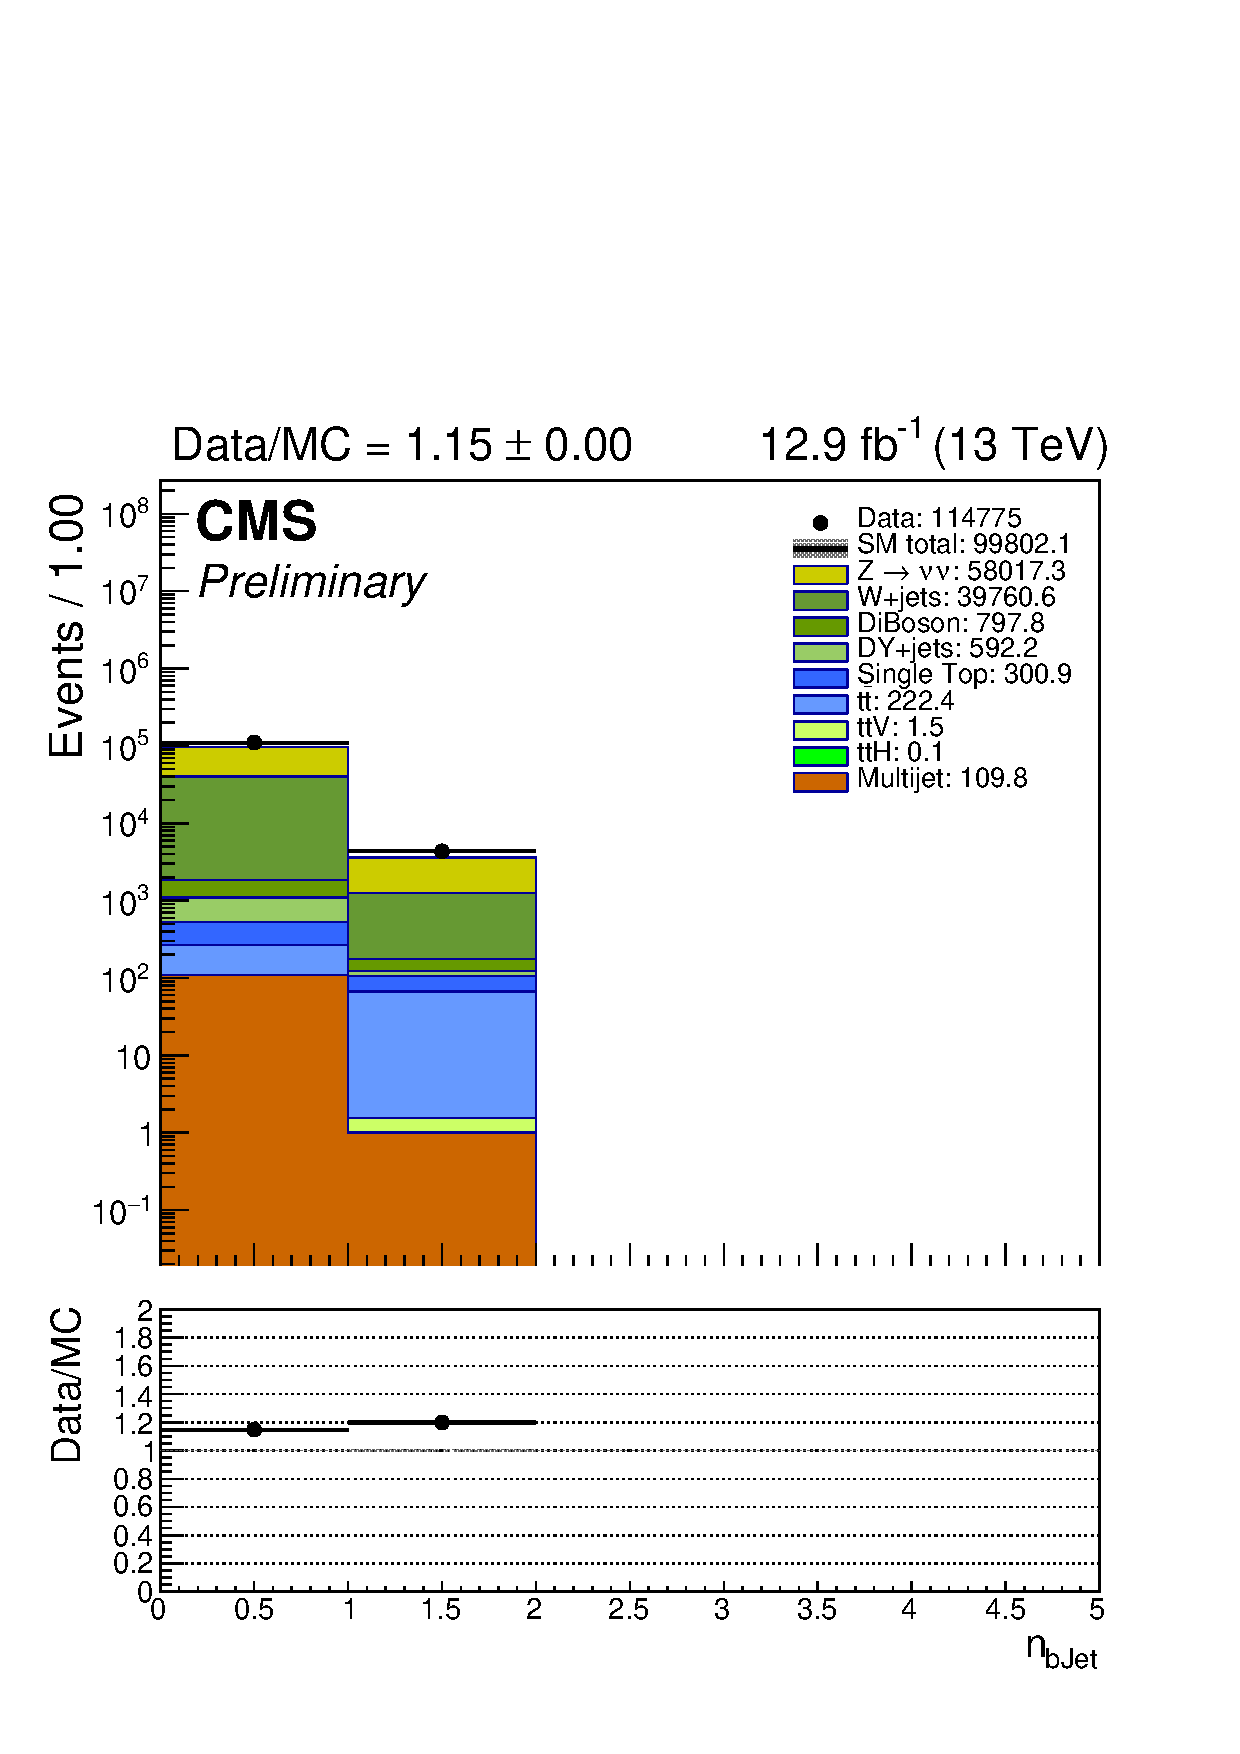
\includegraphics[width=0.5\textwidth]{figs/analysis/distributions/Signal/nBJet40_eq1j.pdf}} ~~
        \subfloat {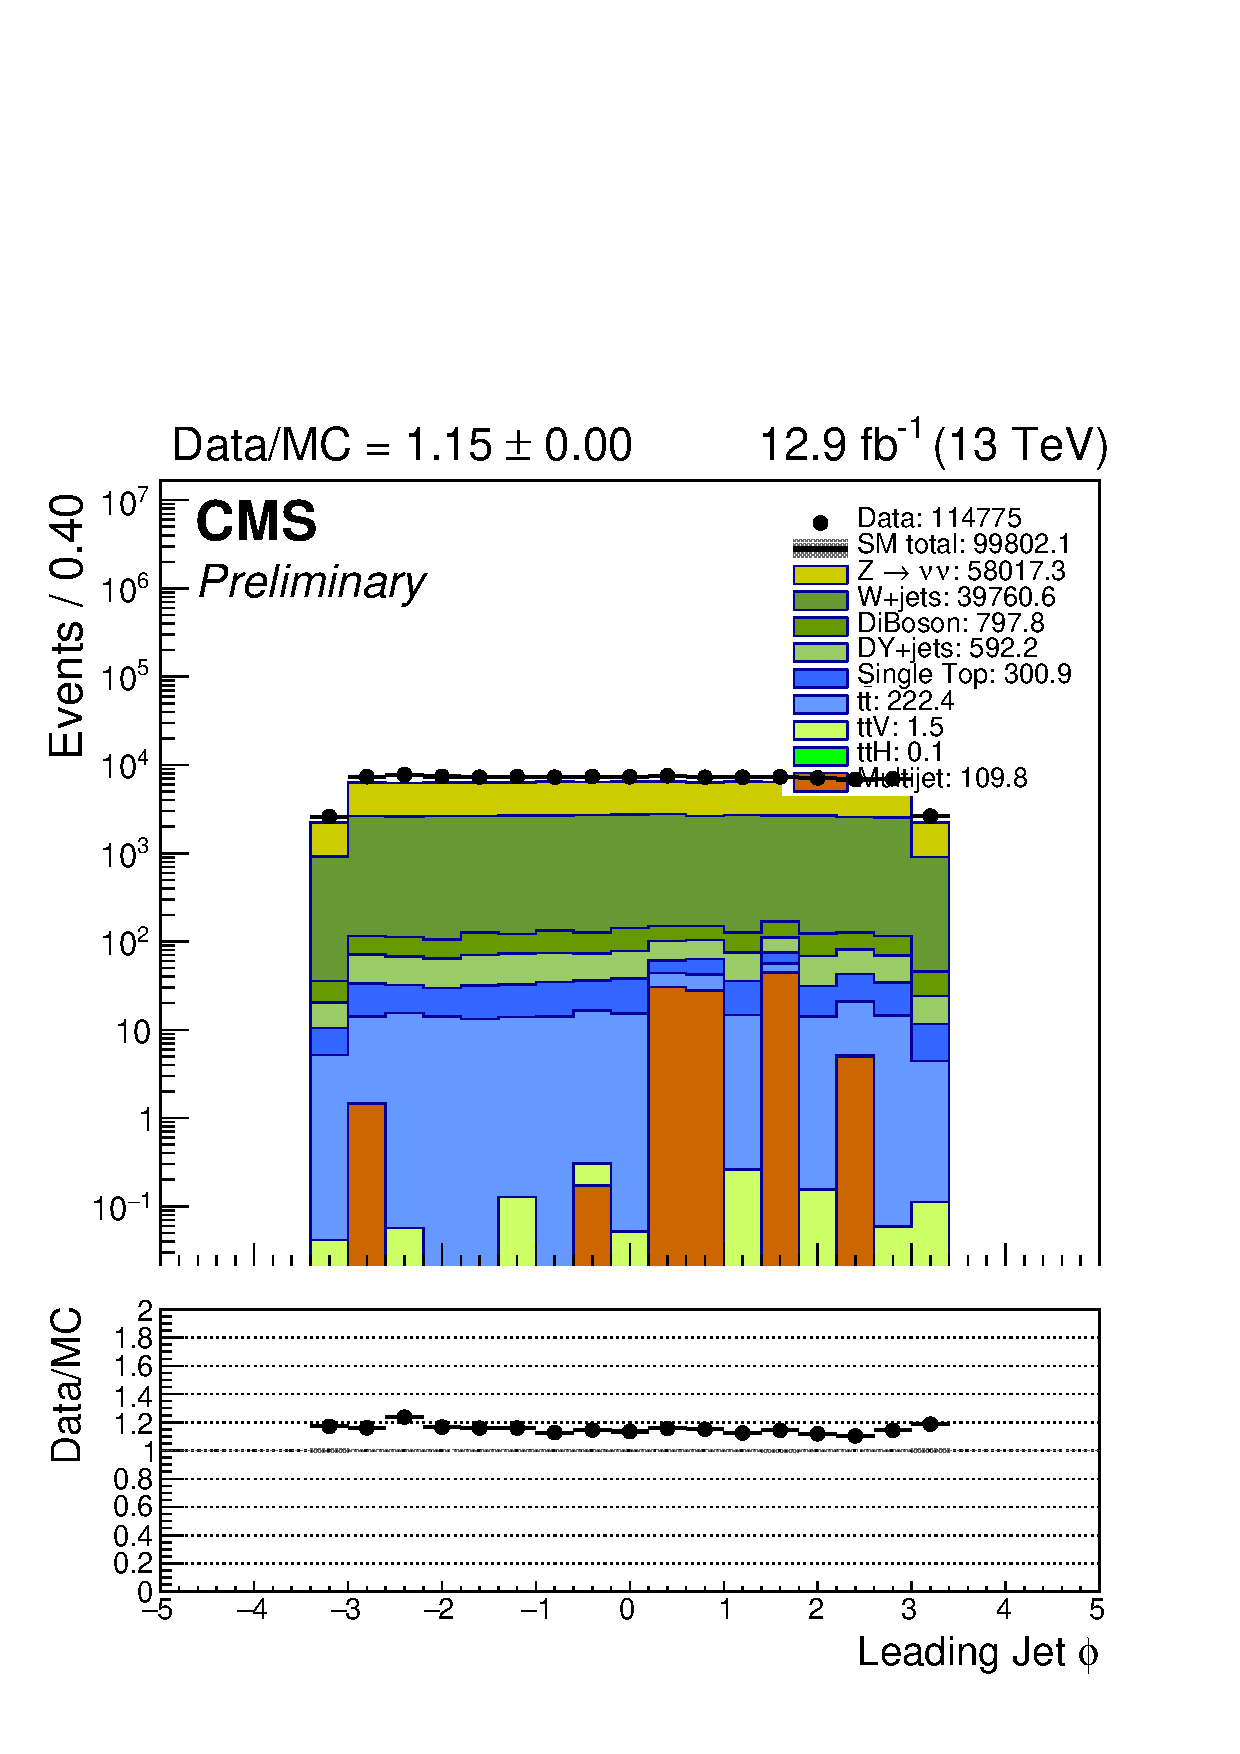
\includegraphics[width=0.5\textwidth]{figs/analysis/distributions/Signal/jet_phi[0]_eq1j.pdf}} \\
        \caption{Key analysis variables for hadronic signal region (monojet bins)}
        \label{fig:distribution_signal_mono}
    \end{center}
\end{figure}

\clearpage
\section{Binning of \MHT dimension}
\label{app:mhtBinning} 
In Tab. \ref{tab:mhtBins_eq2j}-\ref{tab:mhtBins_ge5a} the binning of
the \mht dimension for all the categories used in the analysis is
presented, for the asymmetric and symmetric topologies respectively.
Where the binning is not specified no template is used.  For the
monojet category no template is used. 

\begin{table}[h!]
  \scriptsize
  \centering
  \caption{The \mht binning for the jet category $n_{jet} = 2$. 
  \label{tab:mhtBins_eq2j}}
  \begin{tabular}{ lll }
    Jet category & $H_{T}$ bin & \mht template binning (GeV) \\ \hline

    \hline
    $\njet = 2 \;, \nb = 0 $ & $200 < H_{T} < 250$ GeV & 130, 175, 225 \\ 
     & $250 < H_{T} < 300$ GeV & 130, 175, 225, 275 \\ 
     & $300 < H_{T} < 350$ GeV & 130, 175, 225, 275, 325 \\ 
     & $350 < H_{T} < 400$ GeV & 130, 175, 225, 275, 325, 375 \\ 
     & $400 < H_{T} < 500$ GeV & 130, 175, 225, 275, 325, 375, 425, 475 \\ 
     & $500 < H_{T} < 600$ GeV & 130, 175, 225, 275, 325, 375, 425, 475, 525, 575 \\ 
     & $600 < H_{T} < 800$ GeV & 130, 175, 225, 275, 325, 375, 425, 475, 525, 575, 625, 675, 725, 775 \\ 
     & $H_{T} > 800$ GeV & 130, 250, 300, 350, 400, 450, 500, 550, 600, 650, 700, 750, 800 \\ 
    \hline
    $\njet = 2 \;, \nb = 1$ & $200 < H_{T} < 250$ GeV & 130, 175, 225 \\ 
     & $250 < H_{T} < 300$ GeV & 130, 175, 225, 275 \\ 
     & $300 < H_{T} < 350$ GeV & 130, 175, 225, 275, 325 \\ 
     & $350 < H_{T} < 400$ GeV & 130, 175, 225, 275, 325, 375 \\ 
     & $400 < H_{T} < 500$ GeV & 130, 175, 225, 275, 325, 375, 425, 475 \\ 
     & $500 < H_{T} < 600$ GeV & 130, 225, 275, 325, 375, 425, 475, 525, 575 \\ 
     & $600 < H_{T} < 800$ GeV & 130, 225, 275, 325, 375, 425, 475, 525, 575, 675, 725, 775 \\ 
     & $H_{T} > 800$ GeV & 130, 250, 300, 350, 400, 450, 500, 550, 600, 650, 700, 750, 800 \\ 
    \hline
    $\njet = 2 \;, \nb = 2 $ & $200 < H_{T} < 250$ GeV & - \\ 
     & $250 < H_{T} < 300$ GeV & 130, 175, 225, 275 \\ 
     & $300 < H_{T} < 350$ GeV & - \\ 
     & $350 < H_{T} < 400$ GeV & 130, 250, 300, 350 \\ 
     & $400 < H_{T} < 500$ GeV & - \\ 
     & $500 < H_{T} < 600$ GeV & 130, 225, 325, 375, 475, 525, 575 \\ 
     & $H_{T} > 600$ GeV & - \\ 

  \end{tabular}
\end{table}



\begin{table}[h!]
  \scriptsize
  \centering
  \caption{The \mht binning for the jet category $n_{jet} = 3$. 
  \label{tab:mhtBins_eq3j}}
  \begin{tabular}{ lll }
    Jet category & $H_{T}$ bin & \mht template binning (GeV) \\ \hline

    \hline
    $\njet = 3 \;, \nb = 0 $ & $200 < H_{T} < 250$ GeV & 130, 225 \\ 
     & $250 < H_{T} < 300$ GeV & 130, 175, 225, 275 \\ 
     & $300 < H_{T} < 350$ GeV & 130, 175, 225, 275, 325 \\ 
     & $350 < H_{T} < 400$ GeV & 130, 175, 225, 275, 325, 375 \\ 
     & $400 < H_{T} < 500$ GeV & 130, 175, 225, 275, 325, 375, 425, 475 \\ 
     & $500 < H_{T} < 600$ GeV & 130, 175, 225, 275, 325, 375, 425, 475, 525, 575 \\ 
     & $600 < H_{T} < 800$ GeV & 130, 225, 275, 325, 375, 425, 475, 525, 575, 625, 675, 725, 775 \\ 
     & $H_{T} > 800$ GeV & 130, 200, 250, 300, 350, 400, 450, 500, 550, 600, 650, 700, 750, 800 \\ 
    \hline
    $\njet = 3 \;, \nb = 1$ & $250 < H_{T} < 300$ GeV & 130, 175, 225, 275 \\ 
     & $300 < H_{T} < 350$ GeV & 130, 175, 225, 275, 325 \\ 
     & $350 < H_{T} < 400$ GeV & 130, 175, 225, 275, 325, 375 \\ 
     & $400 < H_{T} < 500$ GeV & 130, 175, 225, 275, 325, 375, 425, 475 \\ 
     & $500 < H_{T} < 600$ GeV & 130, 175, 225, 275, 325, 375, 425, 475, 525, 575 \\ 
     & $600 < H_{T} < 800$ GeV & 130, 225, 275, 325, 375, 425, 475, 525, 575, 625, 675, 725, 775 \\ 
     & $H_{T} > 800$ GeV & 130, 200, 250, 300, 350, 400, 450, 500, 550, 600, 650, 700, 750, 800 \\ 
    \hline
    $\njet = 3 \;, \nb = 2 $ & $250 < H_{T} < 300$ GeV & 130, 225, 275 \\ 
     & $300 < H_{T} < 350$ GeV & 130, 175, 225, 275, 325 \\ 
     & $350 < H_{T} < 400$ GeV & 130, 175, 225, 275, 325, 375 \\ 
     & $400 < H_{T} < 500$ GeV & 130, 175, 225, 275, 325, 375, 425 \\ 
     & $500 < H_{T} < 600$ GeV & 130, 200, 250, 300, 425, 475, 525, 575 \\ 
     & $600 < H_{T} < 800$ GeV & 130, 200, 250, 350, 400, 450, 500, 550, 600, 650, 700, 750 \\ 
     & $H_{T} > 800$ GeV & - \\ 
    \hline
    $\njet = 3 \;, \nb \geq 3$ & $250 < H_{T} < 300$ GeV & - \\ 
     & $350 < H_{T} < 400$ GeV & - \\ 
     & $H_{T} > 400$ GeV & - \\ 

  \end{tabular}
\end{table}



\begin{table}[h!]
  \scriptsize
  \centering
  \caption{The \mht binning for the jet category $n_{jet} = 4$. 
  \label{tab:mhtBins_eq4j}}
  \begin{tabular}{ lll }
    Jet category & $H_{T}$ bin & \mht template binning (GeV) \\ \hline

    \hline
    $\njet = 4 \;, \nb = 0 $ & $250 < H_{T} < 300$ GeV & - \\ 
     & $300 < H_{T} < 350$ GeV & 130, 175, 225, 275, 325 \\ 
     & $350 < H_{T} < 400$ GeV & 130, 175, 225, 275, 325, 375 \\ 
     & $400 < H_{T} < 500$ GeV & 130, 150, 200, 250, 300, 350, 400, 450 \\ 
     & $500 < H_{T} < 600$ GeV & 130, 175, 225, 275, 325, 375, 425, 475, 525, 575 \\ 
     & $600 < H_{T} < 800$ GeV & 130, 200, 250, 300, 350, 400, 450, 500, 550, 600, 650, 700, 750 \\ 
     & $H_{T} > 800$ GeV & 130, 150, 200, 250, 300, 350, 400, 450, 500, 550, 600, 650, 700, 750, 800 \\ 
    \hline
    $\njet = 4 \;, \nb = 1$ & $250 < H_{T} < 300$ GeV & - \\ 
     & $300 < H_{T} < 350$ GeV & 130, 175, 225, 275, 325 \\ 
     & $350 < H_{T} < 400$ GeV & 130, 150, 200, 250, 300, 350 \\ 
     & $400 < H_{T} < 500$ GeV & 130, 150, 200, 250, 300, 350, 400, 450 \\ 
     & $500 < H_{T} < 600$ GeV & 130, 175, 225, 275, 325, 375, 425, 475, 525 \\ 
     & $600 < H_{T} < 800$ GeV & 130, 250, 300, 350, 400, 450, 500, 550, 600, 650, 700, 750 \\ 
     & $H_{T} > 800$ GeV & 130, 150, 200, 250, 300, 350, 400, 450, 500, 550, 600, 650, 700, 750, 800 \\ 
    \hline
    $\njet = 4 \;, \nb = 2 $ & $250 < H_{T} < 300$ GeV & - \\ 
     & $300 < H_{T} < 350$ GeV & 130, 150, 200, 250, 300 \\ 
     & $350 < H_{T} < 400$ GeV & 130, 175, 225, 275, 325 \\ 
     & $400 < H_{T} < 500$ GeV & 130, 150, 200, 250, 300, 350, 400, 450 \\ 
     & $500 < H_{T} < 600$ GeV & 130, 200, 250, 300, 350, 400, 450, 500 \\ 
     & $600 < H_{T} < 800$ GeV & 130, 225, 275, 325, 375, 425, 475, 525, 575, 625, 675, 725 \\ 
     & $H_{T} > 800$ GeV & 130, 200, 250, 300, 350, 400, 450, 500, 550, 600, 650, 700, 750, 800 \\ 
    \hline
    $\njet = 4 \;, \nb \geq 3$ & $350 < H_{T} < 400$ GeV & - \\ 
     & $400 < H_{T} < 500$ GeV & - \\ 
     & $500 < H_{T} < 600$ GeV & 130, 300, 400 \\ 
     & $600 < H_{T} < 800$ GeV & - \\ 
     & $H_{T} > 800$ GeV & - \\ 

  \end{tabular}
\end{table}



\begin{table}[h!]
  \scriptsize
  \centering
  \caption{The \mht binning for the jet category $n_{jet} = 5$. 
  \label{tab:mhtBins_ge5j}}
  \begin{tabular}{ lll }
    Jet category & $H_{T}$ bin & \mht template binning (GeV) \\ \hline

    \hline
    $\njet \geq 5 \;, \nb = 0$ & $350 < H_{T} < 400$ GeV & 130, 150, 200, 250, 300, 350 \\ 
     & $400 < H_{T} < 500$ GeV & 130, 150, 200, 250, 300, 350, 400, 450 \\ 
     & $500 < H_{T} < 600$ GeV & 130, 175, 225, 275, 325, 375, 425, 475, 525 \\ 
     & $600 < H_{T} < 800$ GeV & 130, 200, 250, 300, 350, 400, 450, 500, 550, 600, 650, 700, 750 \\ 
     & $H_{T} > 800$ GeV & 130, 150, 200, 250, 300, 350, 400, 450, 500, 550, 600, 650, 700, 750, 800 \\ 
    \hline
    $\njet \geq 5 \;, \nb = 1$ & $350 < H_{T} < 400$ GeV & 130, 150, 200, 250, 300 \\ 
     & $400 < H_{T} < 500$ GeV & 130, 175, 225, 275, 325, 375, 425 \\ 
     & $500 < H_{T} < 600$ GeV & 130, 175, 225, 275, 325, 375, 425, 475, 525 \\ 
     & $600 < H_{T} < 800$ GeV & 130, 225, 275, 325, 375, 425, 475, 525, 575, 625, 675, 725 \\ 
     & $H_{T} > 800$ GeV & 130, 150, 200, 250, 300, 350, 400, 450, 500, 550, 600, 650, 700, 750, 800 \\ 
    \hline
    $\njet \geq 5 \;, \nb = 2$ & $350 < H_{T} < 400$ GeV & 130, 175, 225, 275 \\ 
     & $400 < H_{T} < 500$ GeV & 130, 150, 200, 250, 300, 350 \\ 
     & $500 < H_{T} < 600$ GeV & 130, 200, 250, 300, 350, 400, 450 \\ 
     & $600 < H_{T} < 800$ GeV & 130, 200, 250, 300, 350, 400, 450, 500, 550, 600, 650 \\ 
     & $H_{T} > 800$ GeV & 130, 150, 200, 250, 300, 350, 400, 450, 500, 550, 600, 650, 700, 750, 800 \\ 
    \hline
    $\njet \geq 5 \;, \nb \geq 3$ & $400 < H_{T} < 500$ GeV & - \\ 
     & $500 < H_{T} < 600$ GeV & - \\ 
     & $600 < H_{T} < 800$ GeV & 130, 225, 275, 325, 375, 425, 475, 525, 575 \\ 
     & $H_{T} > 800$ GeV & 130, 200, 250, 300, 350, 400, 450, 500, 550, 650, 700, 800 \\ 

  \end{tabular}
\end{table}



\begin{table}[h!]
  \scriptsize
  \centering
  \caption{The \mht binning for the jet category $n_{jet}^{asym} = 2$. 
  \label{tab:mhtBins_eq2a}}
  \begin{tabular}{ lll }
    Jet category & $H_{T}$ bin & \mht template binning (GeV) \\ \hline

    \hline
    $\njet^{\mathrm{asy}}  =   2 \;, \nb = 0 $ & $200 < H_{T} < 250$ GeV & 130, 175, 225 \\ 
     & $250 < H_{T} < 300$ GeV & 130, 225, 275 \\ 
     & $300 < H_{T} < 350$ GeV & 130, 275, 325 \\ 
     & $350 < H_{T} < 400$ GeV & 130, 325, 375 \\ 
     & $400 < H_{T} < 500$ GeV & 130, 375, 425, 475 \\ 
     & $500 < H_{T} < 600$ GeV & 130, 525, 575 \\ 
     & $H_{T} > 600$ GeV & 130, 600, 650, 700, 750, 800 \\ 
    \hline
    $\njet^{\mathrm{asy}}  =   2 \;, \nb = 1$ & $200 < H_{T} < 250$ GeV & 130, 175, 225 \\ 
     & $250 < H_{T} < 300$ GeV & 130, 225, 275 \\ 
     & $300 < H_{T} < 350$ GeV & 130, 275, 325 \\ 
     & $350 < H_{T} < 400$ GeV & 130, 375 \\ 
     & $400 < H_{T} < 500$ GeV & 130, 425, 475 \\ 
     & $H_{T} > 500$ GeV & - \\ 
    \hline
    $\njet^{\mathrm{asy}}  =   2 \;, \nb = 2$ & $200 < H_{T} < 250$ GeV & 130, 175, 225 \\ 
     & $250 < H_{T} < 300$ GeV & 130, 225, 275 \\ 
     & $300 < H_{T} < 350$ GeV & 130, 325 \\ 
     & $350 < H_{T} < 400$ GeV & - \\ 
     & $H_{T} > 400$ GeV & - \\ 

  \end{tabular}
\end{table}



\begin{table}[h!]
  \scriptsize
  \centering
  \caption{The \mht binning for the jet category $n_{jet}^{asym} = 3$. 
  \label{tab:mhtBins_eq3a}}
  \begin{tabular}{ lll }
    Jet category & $H_{T}$ bin & \mht template binning (GeV) \\ \hline

    \hline
    $\njet^{\mathrm{asy}}  =   3 \;, \nb = 0 $ & $200 < H_{T} < 250$ GeV & 130, 175, 225 \\ 
     & $250 < H_{T} < 300$ GeV & 130, 175, 225, 275 \\ 
     & $300 < H_{T} < 350$ GeV & 130, 175, 225, 275, 325 \\ 
     & $350 < H_{T} < 400$ GeV & 130, 175, 225, 275, 325, 375 \\ 
     & $400 < H_{T} < 500$ GeV & 130, 225, 275, 325, 375, 425, 475 \\ 
     & $500 < H_{T} < 600$ GeV & 130, 425, 475, 525, 575 \\ 
     & $H_{T} > 600$ GeV & 130, 550, 600, 650, 700, 750, 800 \\ 
    \hline
    $\njet^{\mathrm{asy}}  =   3 \;, \nb = 1$ & $200 < H_{T} < 250$ GeV & 130, 175, 225 \\ 
     & $250 < H_{T} < 300$ GeV & 130, 175, 225, 275 \\ 
     & $300 < H_{T} < 350$ GeV & 130, 175, 225, 275, 325 \\ 
     & $350 < H_{T} < 400$ GeV & 130, 175, 225, 275, 325, 375 \\ 
     & $400 < H_{T} < 500$ GeV & 130, 225, 275, 325, 375, 425, 475 \\ 
     & $500 < H_{T} < 600$ GeV & 130, 450, 500, 550 \\ 
     & $H_{T} > 600$ GeV & 130, 550, 600, 650, 700, 750, 800 \\ 
    \hline
    $\njet^{\mathrm{asy}}  =   3 \;, \nb = 2$ & $200 < H_{T} < 250$ GeV & 130, 175, 225 \\ 
     & $250 < H_{T} < 300$ GeV & 130, 175, 225, 275 \\ 
     & $300 < H_{T} < 350$ GeV & 130, 175, 225, 275, 325 \\ 
     & $350 < H_{T} < 400$ GeV & 130, 250, 300, 350 \\ 
     & $400 < H_{T} < 500$ GeV & 130, 275, 325, 375, 425 \\ 
     & $H_{T} > 500$ GeV & 130, 575, 650, 700, 750, 800 \\ 
    \hline
    $\njet^{\mathrm{asy}}  =   3 \;, \nb \geq 3$ & $200 < H_{T} < 250$ GeV & - \\ 
     & $250 < H_{T} < 300$ GeV & - \\ 
     & $H_{T} > 300$ GeV & - \\ 

  \end{tabular}
\end{table}



\begin{table}[h!]
  \scriptsize
  \centering
  \caption{The \mht binning for the jet category $n_{jet}^{asym} = 4$. 
  \label{tab:mhtBins_eq4a}}
  \begin{tabular}{ lll }
    Jet category & $H_{T}$ bin & \mht template binning (GeV) \\ \hline

    \hline
    $\njet^{\mathrm{asy}}  =   4 \;, \nb = 0 $ & $200 < H_{T} < 250$ GeV & 130, 175, 225 \\ 
     & $250 < H_{T} < 300$ GeV & 130, 175, 225, 275 \\ 
     & $300 < H_{T} < 350$ GeV & 130, 175, 225, 275, 325 \\ 
     & $350 < H_{T} < 400$ GeV & 130, 175, 225, 275, 325, 375 \\ 
     & $400 < H_{T} < 500$ GeV & 130, 150, 200, 250, 300, 350, 400, 450 \\ 
     & $500 < H_{T} < 600$ GeV & 130, 250, 300, 350, 400, 450, 500, 550 \\ 
     & $H_{T} > 600$ GeV & 130, 450, 500, 550, 600, 650, 700, 750, 800 \\ 
    \hline
    $\njet^{\mathrm{asy}}  =   4 \;, \nb = 1$ & $200 < H_{T} < 250$ GeV & - \\ 
     & $250 < H_{T} < 300$ GeV & 130, 175, 225, 275 \\ 
     & $300 < H_{T} < 350$ GeV & 130, 175, 225, 275, 325 \\ 
     & $350 < H_{T} < 400$ GeV & 130, 150, 200, 250, 300, 350 \\ 
     & $400 < H_{T} < 500$ GeV & 130, 150, 200, 250, 300, 350, 400, 450 \\ 
     & $500 < H_{T} < 600$ GeV & 130, 250, 300, 350, 400, 450, 500, 550 \\ 
     & $H_{T} > 600$ GeV & 130, 500, 550, 600, 650, 700, 750, 800 \\ 
    \hline
    $\njet^{\mathrm{asy}}  =   4 \;, \nb = 2$ & $200 < H_{T} < 250$ GeV & - \\ 
     & $250 < H_{T} < 300$ GeV & 130, 175, 225, 275 \\ 
     & $300 < H_{T} < 350$ GeV & 130, 150, 200, 250, 300 \\ 
     & $350 < H_{T} < 400$ GeV & 130, 175, 225, 275, 325 \\ 
     & $400 < H_{T} < 500$ GeV & 130, 150, 200, 250, 300, 350, 400 \\ 
     & $500 < H_{T} < 600$ GeV & 130, 325, 375, 425, 475, 525 \\ 
     & $H_{T} > 600$ GeV & - \\ 
    \hline
    $\njet^{\mathrm{asy}}  =   4 \;, \nb \geq 3$ & $250 < H_{T} < 300$ GeV & - \\ 
     & $300 < H_{T} < 350$ GeV & - \\ 
     & $350 < H_{T} < 400$ GeV & 130, 175, 225, 275 \\ 
     & $H_{T} > 400$ GeV & - \\ 

  \end{tabular}
\end{table}



\begin{table}[h!]
  \scriptsize
  \centering
  \caption{The \mht binning for the jet category $n_{jet}^{asym} = 5$. 
  \label{tab:mhtBins_ge5a}}
  \begin{tabular}{ lll }
    Jet category & $H_{T}$ bin & \mht template binning (GeV) \\ \hline

    \hline
    $\njet^{\mathrm{asy}} \geq 5 \;, \nb = 0 $ & $250 < H_{T} < 300$ GeV & - \\ 
     & $300 < H_{T} < 350$ GeV & 130, 150, 200, 250, 300 \\ 
     & $350 < H_{T} < 400$ GeV & 130, 150, 200, 250, 300, 350 \\ 
     & $400 < H_{T} < 500$ GeV & 130, 175, 225, 275, 325, 375, 425 \\ 
     & $500 < H_{T} < 600$ GeV & 130, 200, 250, 300, 350, 400, 450, 500, 550 \\ 
     & $H_{T} > 600$ GeV & 130, 250, 300, 350, 400, 450, 500, 550, 600, 650, 700, 750, 800 \\ 
    \hline
    $\njet^{\mathrm{asy}} \geq 5 \;, \nb = 1$ & $250 < H_{T} < 300$ GeV & - \\ 
     & $300 < H_{T} < 350$ GeV & 130, 150, 200, 250, 300 \\ 
     & $350 < H_{T} < 400$ GeV & 130, 175, 225, 275, 325 \\ 
     & $400 < H_{T} < 500$ GeV & 130, 150, 200, 250, 300, 350, 400 \\ 
     & $500 < H_{T} < 600$ GeV & 130, 175, 225, 275, 325, 375, 425, 500 \\ 
     & $H_{T} > 600$ GeV & 130, 225, 275, 325, 375, 450, 500, 550, 600, 650, 700, 750, 800 \\ 
    \hline
    $\njet^{\mathrm{asy}} \geq 5 \;, \nb = 2$ & $250 < H_{T} < 300$ GeV & - \\ 
     & $300 < H_{T} < 350$ GeV & 130, 150, 200, 250 \\ 
     & $350 < H_{T} < 400$ GeV & 130, 150, 200, 250, 300 \\ 
     & $400 < H_{T} < 500$ GeV & 130, 150, 200, 250, 300, 350 \\ 
     & $500 < H_{T} < 600$ GeV & 130, 175, 225, 275, 325, 375, 425 \\ 
     & $H_{T} > 600$ GeV & 130, 275, 325, 375, 450, 500, 600, 700 \\ 
    \hline
    $\njet^{\mathrm{asy}} \geq 5 \;, \nb \geq 3$ & $300 < H_{T} < 350$ GeV & - \\ 
     & $350 < H_{T} < 400$ GeV & 130, 150, 200, 250 \\ 
     & $400 < H_{T} < 500$ GeV & - \\ 
     & $H_{T} > 500$ GeV & - \\ 

  \end{tabular}
\end{table}

\clearpage
\section{Bin labels key}
\label{app:plotKey}

The \nj ~categories are labelled with four letter strings that indicate
the number of jets and the topology, $a$ for asymmetric and $j$ for
symmetric. The \nb categories contain the letter $b$. The number of
jets is represented by the number and is prefixed by either \emph{eq}
corresponding to $=$, or \emph{ge} corresponding to $\geq$.

The \HT bins are labelled based on their lower bin edge in \gev. This
bin extends up to the next \HT bin, with the exception of $800$ which
is open ended for the symmetric category or $600$ which is open ended
for the asymmetric and mono-jet categories.

As an example, \emph{HT250 eq4j} would correspond to the
$250<\HT<300~\gev$ bin with $\nj=4$ and a symmetric topology.
Alternatively, \emph{HT600 ge5a} would correspond to the
$600<\HT<\infty~\gev$ bin with $\nj\geq5$ and an asymmetric topology.

\section{Variation in transfer factors from known systematic
uncertainties}
\label{app:tfSysts}

The variations of the transfer factors after variations of known
sources of systematic uncertainty, as discussed in
Sec.~\ref{sec:simUnc}. These are shown for all relevant transfer
factors from the \gj, \mj and \mmj control samples. The plots are
labelled as described in the key in Appendix~\ref{app:plotKey}.

\begin{figure}[!h]
  \centering
  \subfloat[b-tag SF (heavy) up variation]{
    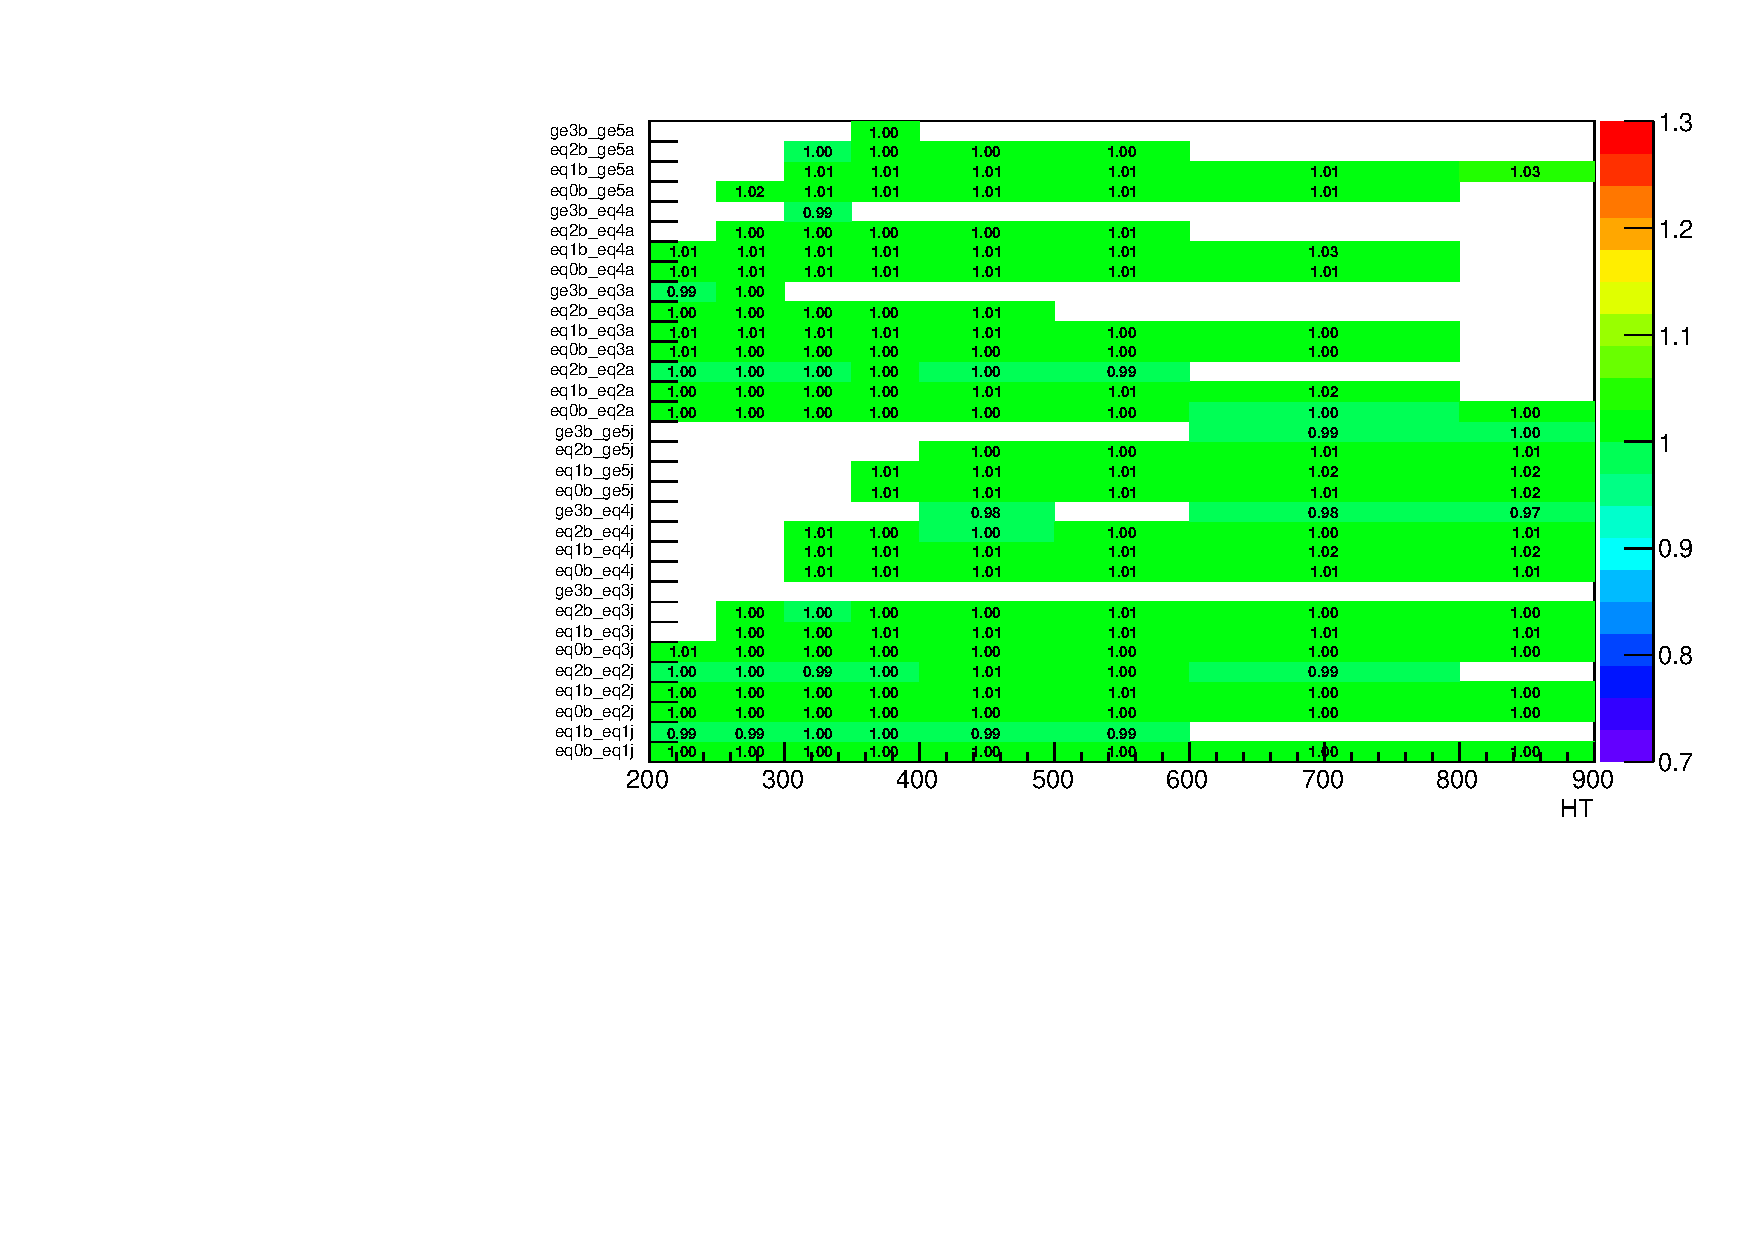
\includegraphics[width=0.5\textwidth]{figs/analysis/systsTf/Zinv/mu/ratiotfh_ht_mht_allbsfWeight_Up.pdf}
  } ~~
  \subfloat[b-tag SF (heavy) down variation]{
    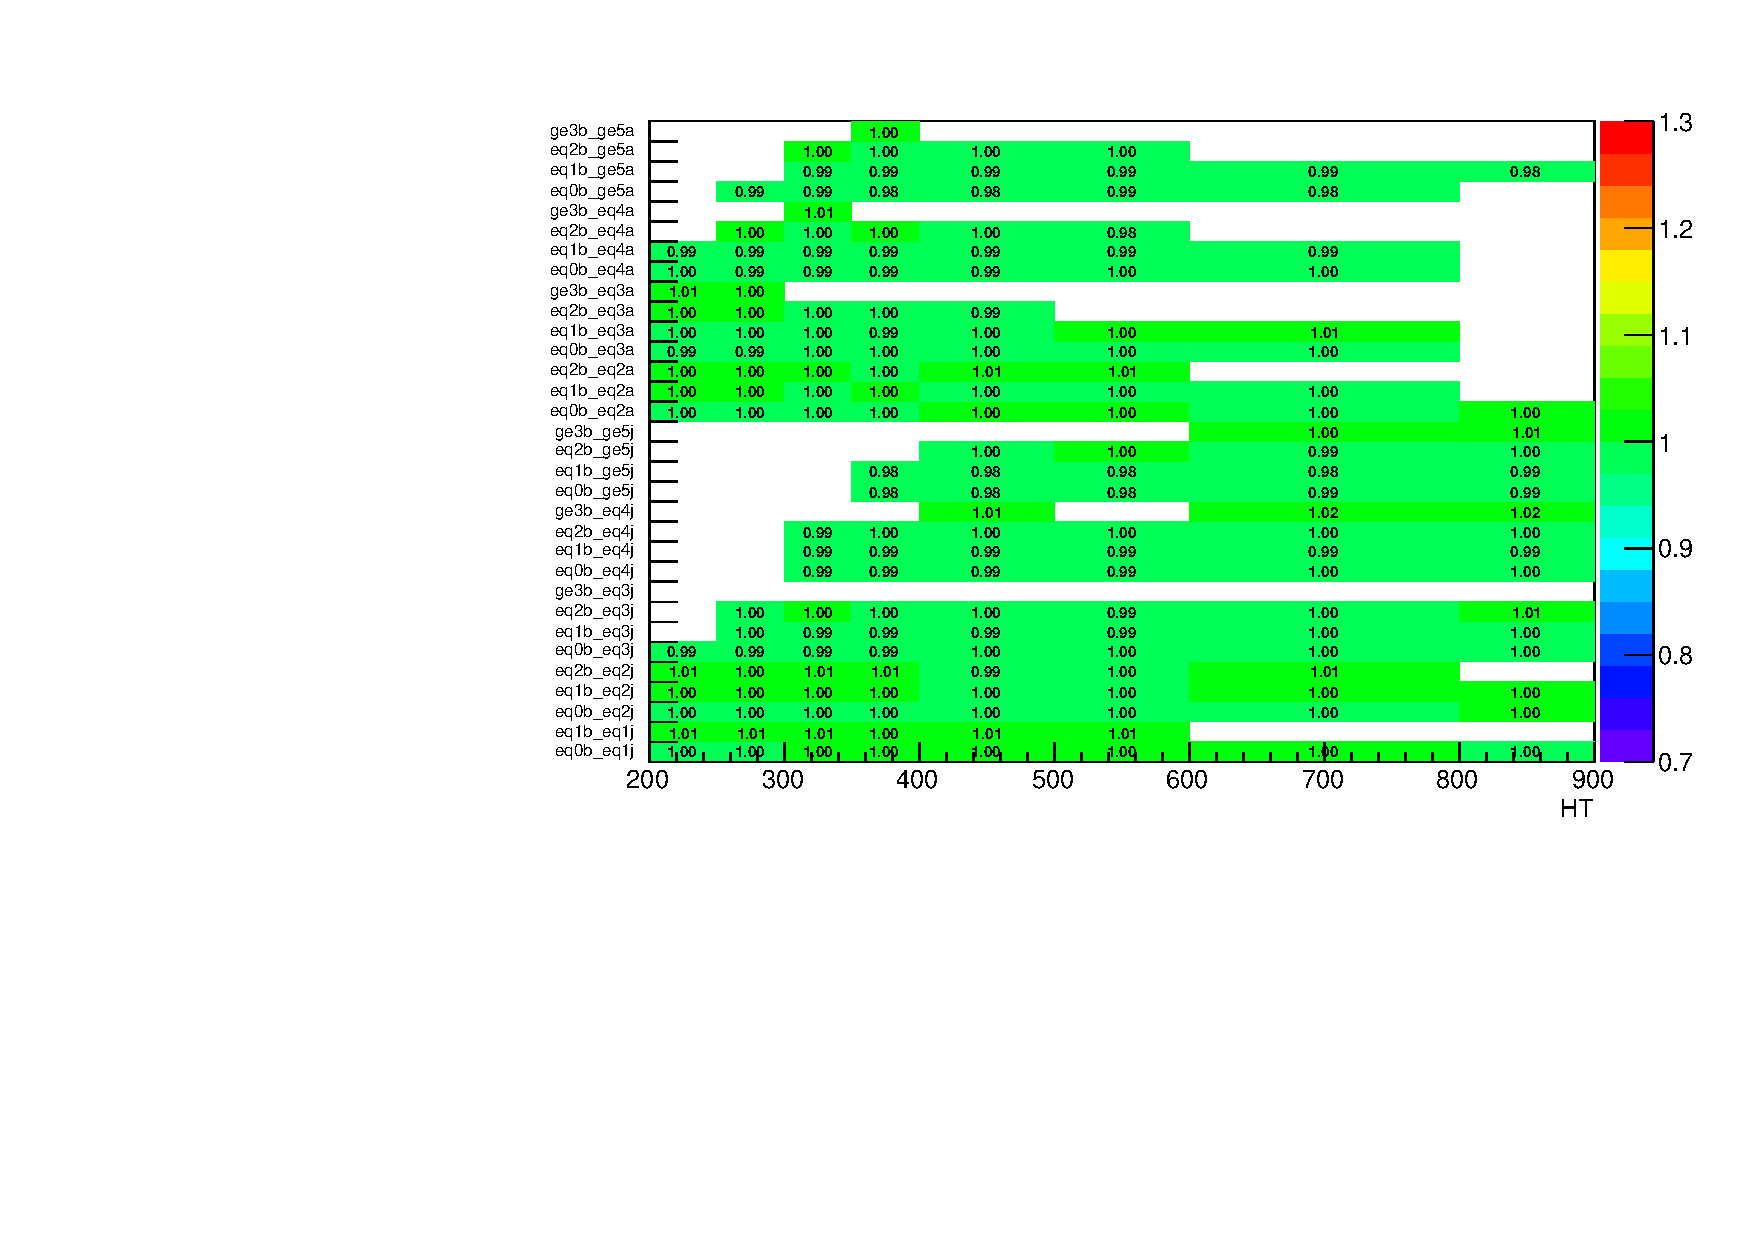
\includegraphics[width=0.5\textwidth]{figs/analysis/systsTf/Zinv/mu/ratiotfh_ht_mht_allbsfWeight_Down.pdf}
  }\\

  \caption{\label{fig:tfSyst_bsf_muToZinv} The relative change in the
  $\mj \rightarrow (\znunu)$ transfer
  factors when varying b-tag SF for heavy jets in MC within its uncertainties, as a function of \scalht and jet category. 
  Variations corresponding to $+1\sigma$ ($-1\sigma$) are shown in the left (right) figure. 
  }
\end{figure}

\begin{figure}[!h]
  \centering
  \subfloat[b-tag SF (heavy) up variation]{
    \includegraphics[width=0.5\textwidth]{figs/analysis/systsTf/Zinv/mumu/ratiotfh_ht_mht_allbsfWeight_Up.pdf}
  } ~~
  \subfloat[b-tag SF (heavy) down variation]{
    \includegraphics[width=0.5\textwidth]{figs/analysis/systsTf/Zinv/mumu/ratiotfh_ht_mht_allbsfWeight_Down.pdf}
  }\\

  \caption{\label{fig:tfSyst_bsf_mumuToZinv} The relative change in
  the $\mmj \rightarrow (\znunu)$ transfer
  factors when varying b-tag SF for heavy jets in MC within its uncertainties, as a function of \scalht and jet category. 
  Variations corresponding to $+1\sigma$ ($-1\sigma$) are shown in the left (right) figure. 
  }
\end{figure}

\begin{figure}[!h]
  \centering
  \subfloat[b-tag SF (heavy) up variation]{
    \includegraphics[width=0.5\textwidth]{figs/analysis/systsTf/Zinv/gj/ratiotfh_ht_mht_allbsfWeight_Up.pdf}
  } ~~
  \subfloat[b-tag SF (heavy) down variation]{
    \includegraphics[width=0.5\textwidth]{figs/analysis/systsTf/Zinv/gj/ratiotfh_ht_mht_allbsfWeight_Down.pdf}
  }\\

  \caption{\label{fig:tfSyst_bsf_gjToZinv} The relative change in the
  $\gj \rightarrow (\znunu)$ transfer
  factors when varying b-tag SF for heavy jets in MC within its uncertainties, as a function of \scalht and jet category. 
  Variations corresponding to $+1\sigma$ ($-1\sigma$) are shown in the left (right) figure. 
  }
\end{figure}

\begin{figure}[!h]
  \centering
  \subfloat[b-tag SF (heavy) up variation]{
    \includegraphics[width=0.5\textwidth]{figs/analysis/systsTf/Ttw/mu/ratiotfh_ht_mht_allbsfWeight_Up.pdf}
  } ~~
  \subfloat[b-tag SF (heavy) down variation]{
    \includegraphics[width=0.5\textwidth]{figs/analysis/systsTf/Ttw/mu/ratiotfh_ht_mht_allbsfWeight_Down.pdf}
  }\\

  \caption{\label{fig:tfSyst_bsf_muToTtw} The relative change in the $\mj \rightarrow \mathrm{tt+W}$ transfer
  factors when varying b-tag SF for heavy jets in MC within its uncertainties, as a function of \scalht and jet category. 
  Variations corresponding to $+1\sigma$ ($-1\sigma$) are shown in the left (right) figure. 
  }
\end{figure}

\clearpage % too many figures, latex doesn't like it

\begin{figure}[!h]
  \centering
  \subfloat[b-tag SF (light) up variation]{
    \includegraphics[width=0.5\textwidth]{figs/analysis/systsTf/Zinv/mu/ratiotfh_ht_mht_allbsfLightWeight_Up.pdf}
  } ~~
  \subfloat[b-tag SF (light) down variation]{
    \includegraphics[width=0.5\textwidth]{figs/analysis/systsTf/Zinv/mu/ratiotfh_ht_mht_allbsfLightWeight_Down.pdf}
  }\\

  \caption{\label{fig:tfSyst_bsfl_muToZinv} The relative change in the
  $\mj \rightarrow (\znunu)$ transfer
  factors when varying b-tag SF for light jets in MC within its uncertainties, as a function of \scalht and jet category. 
  Variations corresponding to $+1\sigma$ ($-1\sigma$) are shown in the left (right) figure. 
  }
\end{figure}

\begin{figure}[!h]
  \centering
  \subfloat[b-tag SF (light) up variation]{
    \includegraphics[width=0.5\textwidth]{figs/analysis/systsTf/Zinv/mumu/ratiotfh_ht_mht_allbsfLightWeight_Up.pdf}
  } ~~
  \subfloat[b-tag SF (light) down variation]{
    \includegraphics[width=0.5\textwidth]{figs/analysis/systsTf/Zinv/mumu/ratiotfh_ht_mht_allbsfLightWeight_Down.pdf}
  }\\

  \caption{\label{fig:tfSyst_bsfl_mumuToZinv} The relative change in
  the $\mmj \rightarrow (\znunu)$ transfer
  factors when varying b-tag SF for light jets in MC within its uncertainties, as a function of \scalht and jet category. 
  Variations corresponding to $+1\sigma$ ($-1\sigma$) are shown in the left (right) figure. 
  }
\end{figure}

\begin{figure}[!h]
  \centering
  \subfloat[b-tag SF (light) up variation]{
    \includegraphics[width=0.5\textwidth]{figs/analysis/systsTf/Zinv/gj/ratiotfh_ht_mht_allbsfLightWeight_Up.pdf}
  } ~~
  \subfloat[b-tag SF (light) down variation]{
    \includegraphics[width=0.5\textwidth]{figs/analysis/systsTf/Zinv/gj/ratiotfh_ht_mht_allbsfLightWeight_Down.pdf}
  }\\

  \caption{\label{fig:tfSyst_bsfl_gjToZinv} The relative change in the
  $\gj \rightarrow (\znunu)$ transfer
  factors when varying b-tag SF for light jets in MC within its uncertainties, as a function of \scalht and jet category. 
  Variations corresponding to $+1\sigma$ ($-1\sigma$) are shown in the left (right) figure. 
  }
\end{figure}

\begin{figure}[!h]
  \centering
  \subfloat[b-tag SF (light) up variation]{
    \includegraphics[width=0.5\textwidth]{figs/analysis/systsTf/Ttw/mu/ratiotfh_ht_mht_allbsfLightWeight_Up.pdf}
  } ~~
  \subfloat[b-tag SF (light) down variation]{
    \includegraphics[width=0.5\textwidth]{figs/analysis/systsTf/Ttw/mu/ratiotfh_ht_mht_allbsfLightWeight_Down.pdf}
  }\\

  \caption{\label{fig:tfSyst_bsfl_muToTtw} The relative change in the $\mj \rightarrow \mathrm{tt+W}$ transfer
  factors when varying b-tag SF for light jets in MC within its uncertainties, as a function of \scalht and jet category. 
  Variations corresponding to $+1\sigma$ ($-1\sigma$) are shown in the left (right) figure. 
  }
\end{figure}



\begin{figure}[!h]
  \centering
  \subfloat[muon scale factor up variation]{
    \includegraphics[width=0.5\textwidth]{figs/analysis/systsTf/Zinv/mu/ratiotfh_ht_mht_allmuonSfWeight_Up.pdf}
  } ~~
  \subfloat[muon scale factor down variation]{
    \includegraphics[width=0.5\textwidth]{figs/analysis/systsTf/Zinv/mu/ratiotfh_ht_mht_allmuonSfWeight_Down.pdf}
  }\\

  \caption{\label{fig:tfSyst_muon scale factor_muToZinv} The relative change in
  the $\mj \rightarrow (\znunu)$ transfer
  factors when varying muon scale factor in MC within its uncertainties, as a function of \scalht and jet category. 
  Variations corresponding to $+1\sigma$ ($-1\sigma$) are shown in the left (right) figure. 
  }
\end{figure}
\begin{figure}[!h]
  \centering
  \subfloat[muon scale factor up variation]{
    \includegraphics[width=0.5\textwidth]{figs/analysis/systsTf/Zinv/mumu/ratiotfh_ht_mht_allmuonSfWeight_Up.pdf}
  } ~~
  \subfloat[muon scale factor down variation]{
    \includegraphics[width=0.5\textwidth]{figs/analysis/systsTf/Zinv/mumu/ratiotfh_ht_mht_allmuonSfWeight_Down.pdf}
  }\\

  \caption{\label{fig:tfSyst_muon scale factor_mumuToZinv} The relative change in
  the $\mmj \rightarrow (\znunu)$ transfer
  factors when varying muon scale factor in MC within its uncertainties, as a function of \scalht and jet category. 
  Variations corresponding to $+1\sigma$ ($-1\sigma$) are shown in the left (right) figure. 
  }
\end{figure}


\begin{figure}[!h]
  \centering
  \subfloat[muon scale factor up variation]{
    \includegraphics[width=0.5\textwidth]{figs/analysis/systsTf/Ttw/mu/ratiotfh_ht_mht_allmuonSfWeight_Up.pdf}
  } ~~
  \subfloat[muon scale factor down variation]{
    \includegraphics[width=0.5\textwidth]{figs/analysis/systsTf/Ttw/mu/ratiotfh_ht_mht_allmuonSfWeight_Down.pdf}
  }\\

  \caption{\label{fig:tfSyst_muon scale factor_muToTtw} The relative change in the $\mj \rightarrow \mathrm{tt+W}$ transfer
  factors when varying muon scale factor in MC within its uncertainties, as a function of \scalht and jet category. 
  Variations corresponding to $+1\sigma$ ($-1\sigma$) are shown in the left (right) figure. 
  }
\end{figure}
\begin{figure}[!h]
  \centering
  \subfloat[Photon trigger weight up variation]{
    \includegraphics[width=0.5\textwidth]{figs/analysis/systsTf/Zinv/gj/ratiotfh_ht_mht_allphotonTriggerWeight_Up.pdf}
  } ~~
  \subfloat[Photon trigger weight down variation]{
    \includegraphics[width=0.5\textwidth]{figs/analysis/systsTf/Zinv/gj/ratiotfh_ht_mht_allphotonTriggerWeight_Down.pdf}
  }\\

  \caption{\label{fig:tfSyst_photonTrigger_gjToZinv} The relative change in
  the $\gj \rightarrow (\znunu)$ transfer
  factors when varying photon trigger weight in MC within its uncertainties, as a function of \scalht and jet category. 
  Variations corresponding to $+1\sigma$ ($-1\sigma$) are shown in the left (right) figure. 
  }
\end{figure}



\begin{figure}[!h]
  \centering
  \subfloat[trigger weight up variation]{
    \includegraphics[width=0.5\textwidth]{figs/analysis/systsTf/Zinv/mu/ratiotfh_ht_mht_alltriggerWeight_Up.pdf}
  } ~~
  \subfloat[trigger weight down variation]{
    \includegraphics[width=0.5\textwidth]{figs/analysis/systsTf/Zinv/mu/ratiotfh_ht_mht_alltriggerWeight_Down.pdf}
  }\\

  \caption{\label{fig:tfSyst_trigger_muToZinv} The relative change in
  the $\mj \rightarrow (\znunu)$ transfer
  factors when varying trigger weight in MC within its uncertainties, as a function of \scalht and jet category. 
  Variations corresponding to $+1\sigma$ ($-1\sigma$) are shown in the left (right) figure. 
  }
\end{figure}
\begin{figure}[!h]
  \centering
  \subfloat[trigger weight up variation]{
    \includegraphics[width=0.5\textwidth]{figs/analysis/systsTf/Zinv/mumu/ratiotfh_ht_mht_alltriggerWeight_Up.pdf}
  } ~~
  \subfloat[trigger weight down variation]{
    \includegraphics[width=0.5\textwidth]{figs/analysis/systsTf/Zinv/mumu/ratiotfh_ht_mht_alltriggerWeight_Down.pdf}
  }\\

  \caption{\label{fig:tfSyst_trigger_mumuToZinv} The relative change in
  the $\mmj \rightarrow (\znunu)$ transfer
  factors when varying trigger weight in MC within its uncertainties, as a function of \scalht and jet category. 
  Variations corresponding to $+1\sigma$ ($-1\sigma$) are shown in the left (right) figure. 
  }
\end{figure}

\begin{figure}[!h]
  \centering
  \subfloat[trigger weight up variation]{
    \includegraphics[width=0.5\textwidth]{figs/analysis/systsTf/Zinv/gj/ratiotfh_ht_mht_alltriggerWeight_Up.pdf}
  } ~~
  \subfloat[trigger weight down variation]{
    \includegraphics[width=0.5\textwidth]{figs/analysis/systsTf/Zinv/gj/ratiotfh_ht_mht_alltriggerWeight_Down.pdf}
  }\\

  \caption{\label{fig:tfSyst_trigger_gjToZinv} The relative change in
  the $\gj \rightarrow (\znunu)$ transfer
  factors when varying trigger weight in MC within its uncertainties, as a function of \scalht and jet category. 
  Variations corresponding to $+1\sigma$ ($-1\sigma$) are shown in the left (right) figure. 
  }
\end{figure}

\begin{figure}[!h]
  \centering
  \subfloat[trigger weight up variation]{
    \includegraphics[width=0.5\textwidth]{figs/analysis/systsTf/Ttw/mu/ratiotfh_ht_mht_alltriggerWeight_Up.pdf}
  } ~~
  \subfloat[trigger weight down variation]{
    \includegraphics[width=0.5\textwidth]{figs/analysis/systsTf/Ttw/mu/ratiotfh_ht_mht_alltriggerWeight_Down.pdf}
  }\\

  \caption{\label{fig:tfSyst_trigger_muToTtw} The relative change in the $\mj \rightarrow \mathrm{tt+W}$ transfer
  factors when varying trigger weight in MC within its uncertainties, as a function of \scalht and jet category. 
  Variations corresponding to $+1\sigma$ ($-1\sigma$) are shown in the left (right) figure. 
  }
\end{figure}

\begin{figure}[!h]
  \centering
  \subfloat[top $p_{T}$ weight up variation]{
    \includegraphics[width=0.5\textwidth]{figs/analysis/systsTf/Zinv/mu/ratiotfh_ht_mht_alltopPtWeight_Up.pdf}
  } ~~
  \subfloat[top $p_{T}$ weight down variation]{
    \includegraphics[width=0.5\textwidth]{figs/analysis/systsTf/Zinv/mu/ratiotfh_ht_mht_alltopPtWeight_Down.pdf}
  }\\

  \caption{\label{fig:tfSyst_topPt_muToZinv} The relative change in
  the $\mj \rightarrow (\znunu)$ transfer
  factors when varying top $p_{T}$ weight in MC within its uncertainties, as a function of \scalht and jet category. 
  Variations corresponding to $+1\sigma$ ($-1\sigma$) are shown in the left (right) figure. 
  }
\end{figure}
\begin{figure}[!h]
  \centering
  \subfloat[top $p_{T}$ weight up variation]{
    \includegraphics[width=0.5\textwidth]{figs/analysis/systsTf/Zinv/mumu/ratiotfh_ht_mht_alltopPtWeight_Up.pdf}
  } ~~
  \subfloat[top $p_{T}$ weight down variation]{
    \includegraphics[width=0.5\textwidth]{figs/analysis/systsTf/Zinv/mumu/ratiotfh_ht_mht_alltopPtWeight_Down.pdf}
  }\\

  \caption{\label{fig:tfSyst_topPt_mumuToZinv} The relative change in
  the $\mmj \rightarrow (\znunu)$ transfer
  factors when varying top $p_{T}$ weight in MC within its uncertainties, as a function of \scalht and jet category. 
  Variations corresponding to $+1\sigma$ ($-1\sigma$) are shown in the left (right) figure. 
  }
\end{figure}

\begin{figure}[!h]
  \centering
  \subfloat[top $p_{T}$ weight up variation]{
    \includegraphics[width=0.5\textwidth]{figs/analysis/systsTf/Ttw/mu/ratiotfh_ht_mht_alltopPtWeight_Up.pdf}
  } ~~
  \subfloat[top $p_{T}$ weight down variation]{
    \includegraphics[width=0.5\textwidth]{figs/analysis/systsTf/Ttw/mu/ratiotfh_ht_mht_alltopPtWeight_Down.pdf}
  }\\

  \caption{\label{fig:tfSyst_topPt_muToTtw} The relative change in the $\mj \rightarrow \mathrm{tt+W}$ transfer
  factors when varying top $p_{T}$ weight in MC within its uncertainties, as a function of \scalht and jet category. 
  Variations corresponding to $+1\sigma$ ($-1\sigma$) are shown in the left (right) figure. 
  }
\end{figure}



\begin{figure}[!h]
  \centering
  \subfloat[PU weight up variation]{
    \includegraphics[width=0.5\textwidth]{figs/analysis/systsTf/Zinv/mu/ratiotfh_ht_mht_allpuWeight_Up.pdf}
  } ~~
  \subfloat[PU weight down variation]{
    \includegraphics[width=0.5\textwidth]{figs/analysis/systsTf/Zinv/mu/ratiotfh_ht_mht_allpuWeight_Down.pdf}
  }\\

  \caption{\label{fig:tfSyst_pu_muToZinv} The relative change in the
  $\mj \rightarrow (\znunu)$ transfer
  factors when varying PU weight in MC within its uncertainties, as a function of \scalht and jet category. 
  Variations corresponding to $+1\sigma$ ($-1\sigma$) are shown in the left (right) figure. 
  }
\end{figure}

\begin{figure}[!h]
  \centering
  \subfloat[PU weight up variation]{
    \includegraphics[width=0.5\textwidth]{figs/analysis/systsTf/Zinv/mumu/ratiotfh_ht_mht_allpuWeight_Up.pdf}
  } ~~
  \subfloat[PU weight down variation]{
    \includegraphics[width=0.5\textwidth]{figs/analysis/systsTf/Zinv/mumu/ratiotfh_ht_mht_allpuWeight_Down.pdf}
  }\\

  \caption{\label{fig:tfSyst_pu_mumuToZinv} The relative change in the
  $\mmj \rightarrow (\znunu)$ transfer
  factors when varying PU weight in MC within its uncertainties, as a function of \scalht and jet category. 
  Variations corresponding to $+1\sigma$ ($-1\sigma$) are shown in the left (right) figure. 
  }
\end{figure}

\begin{figure}[!h]
  \centering
  \subfloat[PU weight up variation]{
    \includegraphics[width=0.5\textwidth]{figs/analysis/systsTf/Zinv/gj/ratiotfh_ht_mht_allpuWeight_Up.pdf}
  } ~~
  \subfloat[PU weight down variation]{
    \includegraphics[width=0.5\textwidth]{figs/analysis/systsTf/Zinv/gj/ratiotfh_ht_mht_allpuWeight_Down.pdf}
  }\\

  \caption{\label{fig:tfSyst_pu_gjToZinv} The relative change in the
  $\gj \rightarrow (\znunu)$ transfer
  factors when varying PU weight in MC within its uncertainties, as a function of \scalht and jet category. 
  Variations corresponding to $+1\sigma$ ($-1\sigma$) are shown in the left (right) figure. 
  }
\end{figure}

\begin{figure}[!h]
  \centering
  \subfloat[PU weight up variation]{
    \includegraphics[width=0.5\textwidth]{figs/analysis/systsTf/Ttw/mu/ratiotfh_ht_mht_allpuWeight_Up.pdf}
  } ~~
  \subfloat[PU weight down variation]{
    \includegraphics[width=0.5\textwidth]{figs/analysis/systsTf/Ttw/mu/ratiotfh_ht_mht_allpuWeight_Down.pdf}
  }\\

  \caption{\label{fig:tfSyst_pu_muToTtw} The relative change in the $\mj \rightarrow \mathrm{tt+W}$ transfer
  factors when varying PU weight in MC within its uncertainties, as a function of \scalht and jet category. 
  Variations corresponding to $+1\sigma$ ($-1\sigma$) are shown in the left (right) figure. 
  }
\end{figure}




\end{appendices}

%% Produce the un-numbered back matter (e.g. colophon,
%% bibliography, tables of figures etc., index...)
\begin{backmatter}
  \begin{colophon}
  This thesis was made in \LaTeXe{} using the ``hepthesis'' class~\cite{hepthesis}.
\end{colophon}

%% You're recommended to use the eprint-aware biblio styles which
%% can be obtained from e.g. www.arxiv.org. The file mythesis.bib
%% is derived from the source using the SPIRES Bibtex service.
\bibliographystyle{h-physrev}
\bibliography{mythesis}

%% I prefer to put these tables here rather than making the
%% front matter seemingly interminable. No-one cares, anyway!
\listoffigures
\listoftables

%% If you have time and interest to generate a (decent) index,
%% then you've clearly spent more time on the write-up than the 
%% research ;-)
%\printindex

\end{backmatter}

%% Close
\end{document}
